\documentclass[]{book}
\usepackage{lmodern}
\usepackage{amssymb,amsmath}
\usepackage{ifxetex,ifluatex}
\usepackage{fixltx2e} % provides \textsubscript
\ifnum 0\ifxetex 1\fi\ifluatex 1\fi=0 % if pdftex
  \usepackage[T1]{fontenc}
  \usepackage[utf8]{inputenc}
\else % if luatex or xelatex
  \ifxetex
    \usepackage{mathspec}
  \else
    \usepackage{fontspec}
  \fi
  \defaultfontfeatures{Ligatures=TeX,Scale=MatchLowercase}
\fi
% use upquote if available, for straight quotes in verbatim environments
\IfFileExists{upquote.sty}{\usepackage{upquote}}{}
% use microtype if available
\IfFileExists{microtype.sty}{%
\usepackage[]{microtype}
\UseMicrotypeSet[protrusion]{basicmath} % disable protrusion for tt fonts
}{}
\PassOptionsToPackage{hyphens}{url} % url is loaded by hyperref
\usepackage[unicode=true]{hyperref}
\hypersetup{
            pdftitle={Differential Gene Expression Analysis},
            pdfauthor={Alexey Larionov},
            pdfborder={0 0 0},
            breaklinks=true}
\urlstyle{same}  % don't use monospace font for urls
\usepackage{natbib}
\bibliographystyle{plainnat}
\usepackage{color}
\usepackage{fancyvrb}
\newcommand{\VerbBar}{|}
\newcommand{\VERB}{\Verb[commandchars=\\\{\}]}
\DefineVerbatimEnvironment{Highlighting}{Verbatim}{commandchars=\\\{\}}
% Add ',fontsize=\small' for more characters per line
\usepackage{framed}
\definecolor{shadecolor}{RGB}{248,248,248}
\newenvironment{Shaded}{\begin{snugshade}}{\end{snugshade}}
\newcommand{\KeywordTok}[1]{\textcolor[rgb]{0.13,0.29,0.53}{\textbf{#1}}}
\newcommand{\DataTypeTok}[1]{\textcolor[rgb]{0.13,0.29,0.53}{#1}}
\newcommand{\DecValTok}[1]{\textcolor[rgb]{0.00,0.00,0.81}{#1}}
\newcommand{\BaseNTok}[1]{\textcolor[rgb]{0.00,0.00,0.81}{#1}}
\newcommand{\FloatTok}[1]{\textcolor[rgb]{0.00,0.00,0.81}{#1}}
\newcommand{\ConstantTok}[1]{\textcolor[rgb]{0.00,0.00,0.00}{#1}}
\newcommand{\CharTok}[1]{\textcolor[rgb]{0.31,0.60,0.02}{#1}}
\newcommand{\SpecialCharTok}[1]{\textcolor[rgb]{0.00,0.00,0.00}{#1}}
\newcommand{\StringTok}[1]{\textcolor[rgb]{0.31,0.60,0.02}{#1}}
\newcommand{\VerbatimStringTok}[1]{\textcolor[rgb]{0.31,0.60,0.02}{#1}}
\newcommand{\SpecialStringTok}[1]{\textcolor[rgb]{0.31,0.60,0.02}{#1}}
\newcommand{\ImportTok}[1]{#1}
\newcommand{\CommentTok}[1]{\textcolor[rgb]{0.56,0.35,0.01}{\textit{#1}}}
\newcommand{\DocumentationTok}[1]{\textcolor[rgb]{0.56,0.35,0.01}{\textbf{\textit{#1}}}}
\newcommand{\AnnotationTok}[1]{\textcolor[rgb]{0.56,0.35,0.01}{\textbf{\textit{#1}}}}
\newcommand{\CommentVarTok}[1]{\textcolor[rgb]{0.56,0.35,0.01}{\textbf{\textit{#1}}}}
\newcommand{\OtherTok}[1]{\textcolor[rgb]{0.56,0.35,0.01}{#1}}
\newcommand{\FunctionTok}[1]{\textcolor[rgb]{0.00,0.00,0.00}{#1}}
\newcommand{\VariableTok}[1]{\textcolor[rgb]{0.00,0.00,0.00}{#1}}
\newcommand{\ControlFlowTok}[1]{\textcolor[rgb]{0.13,0.29,0.53}{\textbf{#1}}}
\newcommand{\OperatorTok}[1]{\textcolor[rgb]{0.81,0.36,0.00}{\textbf{#1}}}
\newcommand{\BuiltInTok}[1]{#1}
\newcommand{\ExtensionTok}[1]{#1}
\newcommand{\PreprocessorTok}[1]{\textcolor[rgb]{0.56,0.35,0.01}{\textit{#1}}}
\newcommand{\AttributeTok}[1]{\textcolor[rgb]{0.77,0.63,0.00}{#1}}
\newcommand{\RegionMarkerTok}[1]{#1}
\newcommand{\InformationTok}[1]{\textcolor[rgb]{0.56,0.35,0.01}{\textbf{\textit{#1}}}}
\newcommand{\WarningTok}[1]{\textcolor[rgb]{0.56,0.35,0.01}{\textbf{\textit{#1}}}}
\newcommand{\AlertTok}[1]{\textcolor[rgb]{0.94,0.16,0.16}{#1}}
\newcommand{\ErrorTok}[1]{\textcolor[rgb]{0.64,0.00,0.00}{\textbf{#1}}}
\newcommand{\NormalTok}[1]{#1}
\usepackage{longtable,booktabs}
% Fix footnotes in tables (requires footnote package)
\IfFileExists{footnote.sty}{\usepackage{footnote}\makesavenoteenv{long table}}{}
\usepackage{graphicx,grffile}
\makeatletter
\def\maxwidth{\ifdim\Gin@nat@width>\linewidth\linewidth\else\Gin@nat@width\fi}
\def\maxheight{\ifdim\Gin@nat@height>\textheight\textheight\else\Gin@nat@height\fi}
\makeatother
% Scale images if necessary, so that they will not overflow the page
% margins by default, and it is still possible to overwrite the defaults
% using explicit options in \includegraphics[width, height, ...]{}
\setkeys{Gin}{width=\maxwidth,height=\maxheight,keepaspectratio}
\IfFileExists{parskip.sty}{%
\usepackage{parskip}
}{% else
\setlength{\parindent}{0pt}
\setlength{\parskip}{6pt plus 2pt minus 1pt}
}
\setlength{\emergencystretch}{3em}  % prevent overfull lines
\providecommand{\tightlist}{%
  \setlength{\itemsep}{0pt}\setlength{\parskip}{0pt}}
\setcounter{secnumdepth}{5}
% Redefines (sub)paragraphs to behave more like sections
\ifx\paragraph\undefined\else
\let\oldparagraph\paragraph
\renewcommand{\paragraph}[1]{\oldparagraph{#1}\mbox{}}
\fi
\ifx\subparagraph\undefined\else
\let\oldsubparagraph\subparagraph
\renewcommand{\subparagraph}[1]{\oldsubparagraph{#1}\mbox{}}
\fi

% set default figure placement to htbp
\makeatletter
\def\fps@figure{htbp}
\makeatother

\usepackage{booktabs}
\usepackage{etoolbox}
\makeatletter
\providecommand{\subtitle}[1]{% add subtitle to \maketitle
  \apptocmd{\@title}{\par {\large #1 \par}}{}{}
}
\makeatother

\title{Differential Gene Expression Analysis}
\providecommand{\subtitle}[1]{}
\subtitle{RNA-seq Data Analysis course, EBI, April 2020}
\author{Alexey Larionov}
\date{2020-04-08}

\begin{document}
\maketitle

{
\setcounter{tocdepth}{1}
\tableofcontents
}
\chapter{Introduction}\label{introduction}

This is a practical tutorial illustrating analysis of Differentially
Expressed Genes (DEGs) in RNA-seq data using \textbf{DESeq2} and
\textbf{edgeR} packages. This tutorial avoids discussing statistical
concepts that underlie the analysis, such as normalization, generalised
regression models, distribution of counts etc. These aspects will be
discussed separately in accompanying lecture slides. The only conceptual
point that we touch here is the \textbf{``borrowing''} of data between
genes during the dispersion (variance) assessment.

\section{Dispersion assessment}\label{dispersion-assessment}

Most of the current tools for Differential Gene Expression analysis in
RNA-seq data (including \textbf{DESeq2} and \textbf{edgeR}) were
developed at the time when RNA-seq was quite expensive, so the
researchers could only analyse a small number of samples (e.g.~less than
10 per group). The small number of samples led to a very large
dispersion (variance) estimates in each separate gene. Thus, the
statisticians had to \textbf{``borrow''} data between samples and genes
to facilitate a meaningful analysis. Initially the statisticians
suggested to estimate ``average'' dispersion using all the genes and
samples together. This provided much narrower estimates. However, it was
open to criticism because the dispersion in RNA-seq counts depends on
the gene expression. Thus, the next step was to model a gene dispersion
using only the genes with similar level of expression. This approach was
adopted in \textbf{edgeR} and in \textbf{DESeq2} packages.

In essense, these packages estimate each individual gene dispersion
using two components:

\begin{enumerate}
\def\labelenumi{\arabic{enumi})}
\tightlist
\item
  the actual dispersion observed for the gene\\
\item
  the dispersion of other genes with a similar level of expression
\end{enumerate}

When the number of samples is sufficiently large, \textbf{DESeq2} and
\textbf{edgeR} put most of the weight on the first component. When the
number of samples is small, the actual dispersion estimates are too
broad for a meaningful analysis, so the final estimate ``shrinks''
toward the second component. In other words, the degree of data
\textbf{``borrowing''} is reduced if a large number of samples is
available.

\section{Bioconductor's tutorials}\label{bioconductors-tutorials}

Currently (in April 2020) Bioconductor provides several good practical
tutorials in RNA-seq Differential gene expresion, including:

\begin{itemize}
\tightlist
\item
  \textbf{DESeq2}:
  \url{https://www.bioconductor.org/packages/devel/workflows/vignettes/rnaseqGene/inst/doc/rnaseqGene.html}\\
\item
  \textbf{edgeR} :
  \url{http://bioconductor.org/packages/release/bioc/vignettes/edgeR/inst/doc/edgeRUsersGuide.pdf}\\
\item
  limma-voom and edgeR:
  \url{https://master.bioconductor.org/packages/release/workflows/vignettes/RNAseq123/inst/doc/limmaWorkflow.html}
\end{itemize}

It is highly advised to study these tutorials along with the present
one. They will provide different perspectives to the analysis and lots
of additional practical information (sometimes, even too much
infromation :) Noteworthy, the \textbf{DESeq2} Bioconductor tutorial
discusses in detail the modern data import packages, like
\textbf{tximport} and \textbf{tximeta} for data input from the modern
pseudo-alignment tools like \textbf{Salmon}.

\section{Default threshiolds}\label{default-threshiolds}

Importantly, the Bioconductor tutorials illustrate the data analysis
using small datasets (typically, less than 10 samples). To provide an
alternative perspective, here we analyse a dataset consisting of
hundreds of samples. This analysis illustrates that some of the
packages' default settings (i.e.~DESeq'2 default \textbf{no-change null
hypothesis} and \textbf{0.1 FDR} threshold) may suggest an
unrealistically large proportion of Differentially Expressed Genes
(DEGs), when a large number of samples is available for significantly
differet biological conditions. For instance, more than a half of the
genes are suggested to be DEGs using the default \textbf{DESeq2}
thresholds in our analysis. Adjusting the thresholds, for instance, to
\textbf{2-fold change} at \textbf{FDR \textless{} 0.01} brings the
number of suggested DEGs to around 10\%, which looks more realistic (and
consistent with a common assumption that DEGs should constitute only a
minority of genes).

\section{TCGA}\label{tcga}

Data for this tutorial was obtained from TCGA project:

\begin{itemize}
\tightlist
\item
  \url{https://portal.gdc.cancer.gov/repository}
\end{itemize}

TCGA provides multiple types of data (including clinical annotations,
germline and somatic DNA-sequencing, RNA-sequencing and epigenomic data)
for multiple types of human cancer. The dataset has data for hundreds of
clinical biopsies for each type of studied cancer, sometimes with paired
normal tissue.

\subsection{TCGA data access}\label{tcga-data-access}

TCGA data, which may identify individual patients (such as raw
sequencing data) are protected. However, RNA-Seq counts at gene-level
are provided with open access. For this tutorial we use a set of
selected TCGA Breast Cancer cases (TCGA-BRCA).

TCGA provides RNA-seq counts in several formats, including raw counts
generated by HTSeq and normalised counts (FPKM and FPKM-UQ normalised).
Importantly, DESeq2 and edgeR require \textbf{raw} counts for analysis.

Selected clinical annotations were extracted from TCGA \textbf{xml}
annotation files using a set of in-house scripts. In addition to
\textbf{xml} files, TCGA provides clinical annotations in plain
tabulated format (\textbf{txt} format). However, these \textbf{txt}
files have less annotations than the source \textbf{xml} files. Also, at
the time of preparing these notes (beginnig of 2020), I experienced some
bugs in retrieval of \textbf{txt} files from TCGA.

\subsection{TCGA RNA-seq pipeline}\label{tcga-rna-seq-pipeline}

Information about TCGA pipeline upstream of the HTSeq counts is
available here:

\begin{itemize}
\tightlist
\item
  \url{https://docs.gdc.cancer.gov/Data/Bioinformatics_Pipelines/Expression_mRNA_Pipeline}
\end{itemize}

The TCGA pipeline represents a good example of cutting-edge RNA-seq
analysis, how it was performed several years ago. Importantly, it says
that RNA-seq counts were generated using \textbf{GENCODE v.22} gene
annotations, which we will use later in this analysis.

\section{Tutorial structure}\label{tutorial-structure}

This tutorial is written in R-markdown, where chunks of code are
combined with the output.

\subsection{Samples and Genes}\label{samples-and-genes}

First we will \textbf{read and explore data for samples and genes}. The
source files include more information than we need, so only the
information required for this analysis will be extracted.

\subsection{DESeq2 analysis}\label{deseq2-analysis}

Then \textbf{the data is imported into the DSEq2 data set} and the
\textbf{dataset is explored}.

As a part of exploration, the data will be variance-normalised, which is
required for \textbf{PCA} and \textbf{Hierarchical Clustering}.
Importantly, this normalization is used \emph{for data exploration
only}. The actual differential expression analysis will use
non-normaliased raw data.

Then the \textbf{differential expression analysis} will be done (DSEq2
does it with just a single line of code :)

Finally the results of differential expression analysis are extracted
and explored: including technical data (\textbf{variance adjustments
plot}), a table with with top differentially extracted genes, and
several ways of visualising the results (\textbf{MA plot},
\textbf{Volcano plot} and \textbf{Hierarchical Clustering}).

Importantly, first we will extract results using the default settings
(H0 of no change at 0.1 FDR), which will suggest unsralisticaly hight
number of DEGs. Then we will adjust the settings (H0 of less than 2-fold
change at 0.01 FDR) to obtain a meaninful result.

\subsection{edgeR analysis}\label{edger-analysis}

A similar analysis will be performed using \textbf{edgeR}, except for
Hierarchical clustering, which will not be repeated using \textbf{edgeR}
data.

\subsection{Comparison of DEGs}\label{comparison-of-degs}

The lists of DEGs be compared between \textbf{DESeq2} and \textbf{edgeR}
to show a reasonable concordance between the methods.

Importantly, this tutorial is not concerned about the biological
interpretation of the results (although the it confirms the previously
known ER-related genes in breast cancer). The aim of this tutorial is to
give an example of a practical use of \textbf{DESeq2} and \textbf{edgeR}
for differential gene analysis in RNA-seq data.

\section{Content of the base folder}\label{content-of-the-base-folder}

The analysis expects a base-folder, which contains sub-folders and files
as ilustrated below:

\begin{center}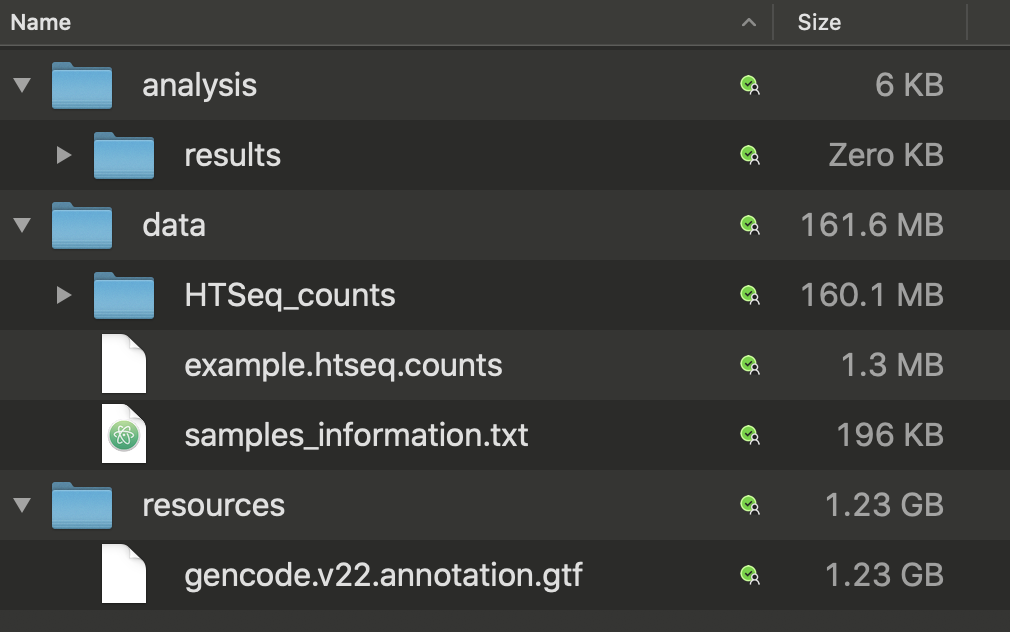
\includegraphics[width=0.5\linewidth]{/Users/alexey/OneDrive/Documents/Teaching/Lecturing/rna-seq-ebi-2020-tutorial/analysis/figures/f01_base_folder} \end{center}

For convinience, the counts data, the samples information file and
gencode.v22 \textbf{gtf} file were downloaded to local storage, as
shown.

\chapter{Setting the Enviroment}\label{setting-the-enviroment}

\section{Required libraries}\label{required-libraries}

This chunk shows how to install the required libraries. The libraries
should be installed just once. So, you dont need to run this chunk again
each time when you run a new analysis. The required packages will
install many dependancies. Importantly, \emph{BiocManager} may require R
version 3.6 or above.

\begin{Shaded}
\begin{Highlighting}[]
\KeywordTok{install.packages}\NormalTok{(}\StringTok{"dplyr"}\NormalTok{) }\CommentTok{# for data wrangling}
\KeywordTok{install.packages}\NormalTok{(}\StringTok{"RColorBrewer"}\NormalTok{) }\CommentTok{# for plotting heatmaps}
\KeywordTok{install.packages}\NormalTok{(}\StringTok{"pheatmap"}\NormalTok{) }\CommentTok{# for plotting heatmaps}
\KeywordTok{install.packages}\NormalTok{(}\StringTok{"VennDiagram"}\NormalTok{) }\CommentTok{# for plotting Venn diagram}

\KeywordTok{install.packages}\NormalTok{(}\StringTok{"BiocManager"}\NormalTok{) }\CommentTok{# for installing Bioconductor packages}
\NormalTok{BiocManager}\OperatorTok{::}\KeywordTok{install}\NormalTok{(}\StringTok{"rtracklayer"}\NormalTok{) }\CommentTok{# for reading GTF file}
\NormalTok{BiocManager}\OperatorTok{::}\KeywordTok{install}\NormalTok{(}\StringTok{"DESeq2"}\NormalTok{) }\CommentTok{# for differential expression analysis}
\end{Highlighting}
\end{Shaded}

\section{Base folder etc}\label{base-folder-etc}

Record the analysis start time, clean-up environment, customise options
and set the \textbf{base folder}

\begin{Shaded}
\begin{Highlighting}[]
\CommentTok{# Start time}
\KeywordTok{Sys.time}\NormalTok{()}
\end{Highlighting}
\end{Shaded}

\begin{verbatim}
## [1] "2020-04-08 16:26:36 BST"
\end{verbatim}

\begin{Shaded}
\begin{Highlighting}[]
\CommentTok{# Intial clean-up}
\KeywordTok{rm}\NormalTok{(}\DataTypeTok{list=}\KeywordTok{ls}\NormalTok{())}
\KeywordTok{graphics.off}\NormalTok{()}

\CommentTok{# Customised options}
\KeywordTok{options}\NormalTok{(}\DataTypeTok{stringsAsFactors =}\NormalTok{ F)}

\CommentTok{# Base folder}
\NormalTok{base_folder=}\StringTok{"/Users/alexey/OneDrive/Documents/Teaching/Lecturing/rna-seq-ebi-2020-tutorial"}
\end{Highlighting}
\end{Shaded}

\chapter{Preparing sample
information}\label{preparing-sample-information}

This chunk reads and explores the samples' information. Then it selects
\textbf{ER-positive} (Estrogen Receptor Positive) and
\textbf{Triple-negative} (Estrogen receptor, Progesterone resceptor and
HER2 negative) tumours. You may try different comparisons, e.g.~the
dataset includes some normal tissue samples paired with tumours.

In addition to the ER status, it keeps \textbf{OCT-imbedding} status.
\textbf{OCT-imbedding} is a small variation in experimental protocol
during RNA extraction. Some of the TCGA BRCA samples were imbedded into
OCT prior RNA extraction, while the others were not imbedded. Thus
\textbf{OCT-imbedding} could be considered a potentially confounding
variable to illustrate dealing with batch effects.

\begin{Shaded}
\begin{Highlighting}[]
\CommentTok{# Read samples information}
\NormalTok{samples_information_file <-}\StringTok{ }\KeywordTok{file.path}\NormalTok{(base_folder,}\StringTok{"data"}\NormalTok{,}\StringTok{"samples_information.txt"}\NormalTok{)}
\NormalTok{samples_information.df <-}\StringTok{ }\KeywordTok{read.table}\NormalTok{(samples_information_file, }\DataTypeTok{header=}\NormalTok{T, }\DataTypeTok{sep=}\StringTok{"}\CharTok{\textbackslash{}t}\StringTok{"}\NormalTok{)}

\CommentTok{# Explore samples information data}
\KeywordTok{dim}\NormalTok{(samples_information.df)}
\end{Highlighting}
\end{Shaded}

\begin{verbatim}
## [1] 629  18
\end{verbatim}

\begin{Shaded}
\begin{Highlighting}[]
\KeywordTok{colnames}\NormalTok{(samples_information.df)}
\end{Highlighting}
\end{Shaded}

\begin{verbatim}
##  [1] "file_id"                 "file_name"               "sample_type"             "sample_oct_embedded"     "bcr_patient_barcode"     "age"                     "menopause_status"        "stage"                   "t"                       "n"                       "m"                       "breast_quadrant"         "histology"               "er"                      "pr"                      "her2"                    "analyte_a260_a280_ratio" "aliquot_concentration"
\end{verbatim}

\begin{Shaded}
\begin{Highlighting}[]
\CommentTok{# Explore samples types }
\KeywordTok{table}\NormalTok{(samples_information.df}\OperatorTok{$}\NormalTok{sample_type)}
\end{Highlighting}
\end{Shaded}

\begin{verbatim}
## 
##       Primary Tumor Solid Tissue Normal 
##                 567                  62
\end{verbatim}

\begin{Shaded}
\begin{Highlighting}[]
\CommentTok{# Select tumours}
\NormalTok{tumours <-}\StringTok{ }\NormalTok{samples_information.df}\OperatorTok{$}\NormalTok{sample_type }\OperatorTok{==}\StringTok{ "Primary Tumor"}

\CommentTok{# Select ER-positive samples}
\NormalTok{er_pos <-}\StringTok{ }\NormalTok{samples_information.df}\OperatorTok{$}\NormalTok{er }\OperatorTok{==}\StringTok{ "Positive"} \OperatorTok{&}\StringTok{ }
\StringTok{          }\NormalTok{samples_information.df}\OperatorTok{$}\NormalTok{pr }\OperatorTok{==}\StringTok{ "Positive"} \OperatorTok{&}\StringTok{ }
\StringTok{          }\NormalTok{samples_information.df}\OperatorTok{$}\NormalTok{her2 }\OperatorTok{==}\StringTok{ "Negative"}

\CommentTok{# Select Triple-negative samples}
\NormalTok{triple_neg <-}\StringTok{ }\NormalTok{samples_information.df}\OperatorTok{$}\NormalTok{er }\OperatorTok{==}\StringTok{ "Negative"} \OperatorTok{&}\StringTok{ }
\StringTok{              }\NormalTok{samples_information.df}\OperatorTok{$}\NormalTok{pr }\OperatorTok{==}\StringTok{ "Negative"} \OperatorTok{&}\StringTok{ }
\StringTok{              }\NormalTok{samples_information.df}\OperatorTok{$}\NormalTok{her2 }\OperatorTok{==}\StringTok{ "Negative"}

\CommentTok{# Combine the conditions and check the count}
\NormalTok{selected_samples <-}\StringTok{ }\NormalTok{tumours }\OperatorTok{&}\StringTok{ }\NormalTok{( er_pos }\OperatorTok{|}\StringTok{ }\NormalTok{triple_neg )}
\KeywordTok{sum}\NormalTok{(selected_samples)}
\end{Highlighting}
\end{Shaded}

\begin{verbatim}
## [1] 238
\end{verbatim}

\begin{Shaded}
\begin{Highlighting}[]
\CommentTok{# Select fields needed for analysis}
\NormalTok{selected_fields <-}\StringTok{ }\KeywordTok{c}\NormalTok{(}\StringTok{"bcr_patient_barcode"}\NormalTok{,}\StringTok{"file_name"}\NormalTok{, }\StringTok{"sample_oct_embedded"}\NormalTok{, }\StringTok{"er"}\NormalTok{)}

\CommentTok{# Keep only selected samples and columns}
\NormalTok{samples.df <-}\StringTok{ }\NormalTok{samples_information.df[selected_samples, selected_fields]}

\CommentTok{# Rename the columns: to make the names concise}
\KeywordTok{colnames}\NormalTok{(samples.df) <-}\StringTok{ }\KeywordTok{c}\NormalTok{(}\StringTok{"patient"}\NormalTok{,}\StringTok{"file"}\NormalTok{,}\StringTok{"oct"}\NormalTok{,}\StringTok{"er"}\NormalTok{) }

\CommentTok{# Check the samples data frame}
\KeywordTok{dim}\NormalTok{(samples.df)}
\end{Highlighting}
\end{Shaded}

\begin{verbatim}
## [1] 238   4
\end{verbatim}

\begin{Shaded}
\begin{Highlighting}[]
\KeywordTok{head}\NormalTok{(samples.df)}
\end{Highlighting}
\end{Shaded}

\begin{verbatim}
##        patient                                                 file   oct       er
## 1 TCGA-A7-A0DA a33029dd-b5fa-4be0-9cbf-971d289146dd.htseq.counts.gz false Negative
## 3 TCGA-D8-A1XU 8d54214a-1d9b-4fea-9c42-5bbb3cd11da9.htseq.counts.gz false Positive
## 5 TCGA-D8-A143 4b19c0e2-2a61-4f0a-9257-4a528e6b320e.htseq.counts.gz false Negative
## 6 TCGA-A7-A4SB cc233ff9-d5fb-4e9b-9007-f58d008df995.htseq.counts.gz false Positive
## 7 TCGA-D8-A1XR bdd8c340-250b-474a-8802-7653b7884ced.htseq.counts.gz false Positive
## 8 TCGA-BH-A18L 5bc7e90d-0fa4-4bde-bee8-4f9b92de03a2.htseq.counts.gz  true Positive
\end{verbatim}

\begin{Shaded}
\begin{Highlighting}[]
\CommentTok{# ER-status vs OCT-embedded }
\KeywordTok{table}\NormalTok{(samples.df[,}\KeywordTok{c}\NormalTok{(}\StringTok{"oct"}\NormalTok{,}\StringTok{"er"}\NormalTok{)])}
\end{Highlighting}
\end{Shaded}

\begin{verbatim}
##        er
## oct     Negative Positive
##   false       23       73
##   true        24      118
\end{verbatim}

\begin{Shaded}
\begin{Highlighting}[]
\CommentTok{# Clean-up}
\KeywordTok{rm}\NormalTok{(samples_information_file, tumours, er_pos, triple_neg, selected_samples, selected_fields, samples_information.df)}
\end{Highlighting}
\end{Shaded}

\chapter{Preparing gene information}\label{preparing-gene-information}

TCGA used the \textbf{gencode.v22.annotation.gtf} annotation file to
generate RNA-seq counts:

\begin{itemize}
\tightlist
\item
  \url{https://docs.gdc.cancer.gov/Data/Bioinformatics_Pipelines/Expression_mRNA_Pipeline}
\end{itemize}

For convinience, this GTF file was downloaded to the resources folder
for this tutorial. However, it can also be downloaded directly from
gencode:

\begin{itemize}
\tightlist
\item
  \url{https://www.gencodegenes.org/human/release_22.html}
\end{itemize}

GTF files can be red into R data-frame using \textbf{readGFF} function
from \textbf{rtracklayer} package.

\subsection{Load required libraries}\label{load-required-libraries}

\textbf{Warnings} and \textbf{messages} printed during the library
loading would clutter the tutorial. Thus they \textbf{are supressed} in
this code. \textbf{This should not be done during actual analysis}
because these Warnings and Messages are important. Thus, many functions
in \emph{genomic packages} may have the same names as \emph{dplyr}
functions. So, ignoring Warnings and Messages may lead to unexpected
interferences.

\begin{Shaded}
\begin{Highlighting}[]
\CommentTok{#install.packages(dplyr)}
\KeywordTok{suppressWarnings}\NormalTok{(}\KeywordTok{suppressMessages}\NormalTok{(}\KeywordTok{library}\NormalTok{(dplyr)))}

\CommentTok{#install.packages("BiocManager")}
\CommentTok{#BiocManager::install("rtracklayer")}
\KeywordTok{suppressWarnings}\NormalTok{(}\KeywordTok{suppressMessages}\NormalTok{(}\KeywordTok{library}\NormalTok{(rtracklayer))) }\CommentTok{# for readGFF()}
\end{Highlighting}
\end{Shaded}

\subsection{Read genes data}\label{read-genes-data}

The genes' Names and IDs \textbf{must} be read from the file that was
used during RNA-seq counts preparation. In case of the TCGA RNA-seq
data, this is \textbf{gencode.v22.annotation.gtf}.

\begin{Shaded}
\begin{Highlighting}[]
\CommentTok{# Read appropriate annotations file}
\NormalTok{gencode_22_file <-}\StringTok{ }\KeywordTok{file.path}\NormalTok{(base_folder,}\StringTok{"resources"}\NormalTok{,}\StringTok{"gencode.v22.annotation.gtf"}\NormalTok{)}
\NormalTok{gencode_}\FloatTok{22.}\NormalTok{df <-}\StringTok{ }\KeywordTok{readGFF}\NormalTok{(gencode_22_file)}

\CommentTok{# Explore the annotations}
\KeywordTok{dim}\NormalTok{(gencode_}\FloatTok{22.}\NormalTok{df)}
\end{Highlighting}
\end{Shaded}

\begin{verbatim}
## [1] 2563671      26
\end{verbatim}

\begin{Shaded}
\begin{Highlighting}[]
\KeywordTok{colnames}\NormalTok{(gencode_}\FloatTok{22.}\NormalTok{df)}
\end{Highlighting}
\end{Shaded}

\begin{verbatim}
##  [1] "seqid"                    "source"                   "type"                     "start"                    "end"                      "score"                    "strand"                   "phase"                    "gene_id"                  "gene_type"                "gene_status"              "gene_name"                "level"                    "havana_gene"              "transcript_id"            "transcript_type"          "transcript_status"        "transcript_name"          "tag"                      "transcript_support_level" "havana_transcript"        "exon_number"              "exon_id"                  "ont"                      "protein_id"               "ccdsid"
\end{verbatim}

\begin{Shaded}
\begin{Highlighting}[]
\CommentTok{# Extract gene_id-s and gene_name-s}
\NormalTok{genes.df <-}\StringTok{ }\NormalTok{gencode_}\FloatTok{22.}\NormalTok{df }\OperatorTok\StringTok{ }
\StringTok{  }\KeywordTok{select}\NormalTok{(gene_id, gene_name) }\OperatorTok\StringTok{ }
\StringTok{  }\KeywordTok{arrange}\NormalTok{(gene_name) }\OperatorTok\StringTok{ }
\StringTok{  }\KeywordTok{distinct}\NormalTok{()}

\CommentTok{# Copy gene IDs to rownames }
\KeywordTok{rownames}\NormalTok{(genes.df) <-}\StringTok{ }\NormalTok{genes.df}\OperatorTok{$}\NormalTok{gene_id}

\CommentTok{# Check result}
\KeywordTok{head}\NormalTok{(genes.df) }\CommentTok{# Interestingly, the gene names are not unique}
\end{Highlighting}
\end{Shaded}

\begin{verbatim}
##                             gene_id gene_name
## ENSG00000275877.1 ENSG00000275877.1 5_8S_rRNA
## ENSG00000276871.1 ENSG00000276871.1 5_8S_rRNA
## ENSG00000252830.2 ENSG00000252830.2   5S_rRNA
## ENSG00000276442.1 ENSG00000276442.1   5S_rRNA
## ENSG00000274408.1 ENSG00000274408.1   5S_rRNA
## ENSG00000274059.1 ENSG00000274059.1   5S_rRNA
\end{verbatim}

\begin{Shaded}
\begin{Highlighting}[]
\KeywordTok{tail}\NormalTok{(genes.df)}
\end{Highlighting}
\end{Shaded}

\begin{verbatim}
##                               gene_id gene_name
## ENSG00000203995.8   ENSG00000203995.8    ZYG11A
## ENSG00000232242.2   ENSG00000232242.2  ZYG11AP1
## ENSG00000162378.11 ENSG00000162378.11    ZYG11B
## ENSG00000159840.14 ENSG00000159840.14       ZYX
## ENSG00000074755.13 ENSG00000074755.13     ZZEF1
## ENSG00000036549.11 ENSG00000036549.11      ZZZ3
\end{verbatim}

\begin{Shaded}
\begin{Highlighting}[]
\CommentTok{# Clean-up}
\KeywordTok{rm}\NormalTok{(gencode_22_file, gencode_}\FloatTok{22.}\NormalTok{df)}
\end{Highlighting}
\end{Shaded}

\chapter{DESeq2 analyisis}\label{deseq2-analyisis}

First, load DESeq2 library. Beware: DESeq2 dependencies may interfere
with \emph{dplyr}. To avoid interference you may use the library name
explicitly, when calling functions, e.g.~use \textbf{DESeq2::plotPCA()}
instead of just \textbf{plotPCA()} (not used in this tutorial).

\begin{Shaded}
\begin{Highlighting}[]
\CommentTok{#install.packages("BiocManager")}
\CommentTok{#BiocManager::install("DESeq2")}
\KeywordTok{suppressWarnings}\NormalTok{(}\KeywordTok{suppressMessages}\NormalTok{(}\KeywordTok{library}\NormalTok{(DESeq2)))}
\end{Highlighting}
\end{Shaded}

\section{DESeqDataSet object}\label{deseqdataset-object}

\subsection{Make DESeqDataSet object}\label{make-deseqdataset-object}

DESeq2 provides several functions for data import from different
upstream tools that generate RNA-seq counts. We use the
\textbf{DESeqDataSetFromHTSeqCount} function that matches the type of
data provided by PCA.

\begin{Shaded}
\begin{Highlighting}[]
\CommentTok{# Set counts folder}
\NormalTok{counts_folder=}\KeywordTok{file.path}\NormalTok{(base_folder,}\StringTok{"data"}\NormalTok{,}\StringTok{"HTSeq_counts"}\NormalTok{)}

\CommentTok{# Make the design variables as factors}
\CommentTok{# (remember: we customised stringsAsFactors to FALSE in the Start section)}
\NormalTok{samples.df}\OperatorTok{$}\NormalTok{oct <-}\StringTok{ }\KeywordTok{as.factor}\NormalTok{(samples.df}\OperatorTok{$}\NormalTok{oct)}
\NormalTok{samples.df}\OperatorTok{$}\NormalTok{er <-}\StringTok{ }\KeywordTok{as.factor}\NormalTok{(samples.df}\OperatorTok{$}\NormalTok{er)}

\CommentTok{# Import sanmples data and counts into DESeqDataSet object}
\CommentTok{# "dds" stands for Deseq-Data-Set}
\NormalTok{dds <-}\StringTok{ }\KeywordTok{DESeqDataSetFromHTSeqCount}\NormalTok{(}\DataTypeTok{sampleTable =}\NormalTok{ samples.df,}
                                  \DataTypeTok{directory =}\NormalTok{ counts_folder,}
                                  \DataTypeTok{design =} \OperatorTok{~}\StringTok{ }\NormalTok{oct }\OperatorTok{+}\StringTok{ }\NormalTok{er)}

\CommentTok{# Clean-up}
\KeywordTok{rm}\NormalTok{(counts_folder)}
\end{Highlighting}
\end{Shaded}

\subsection{Explore DESeqDataSet
object}\label{explore-deseqdataset-object}

In short, the \textbf{DESeqDataSet} object generated by
\textbf{DESeqDataSetFromHTSeqCount} includes the following slots:

\begin{itemize}
\tightlist
\item
  slot for the matrix with \textbf{counts} (a part of the
  \textbf{assays} collection, although no other assays is added when
  reading HTSeq counts)\\
\item
  slot for the samples information (\textbf{colData})\\
\item
  slot for the genes information (\textbf{rowData}). It is empty when
  reading HTSeq counts. To illustrate the use of \textbf{rowData} we
  will manually add the gene names (from gencode.22 GTF file)\\
\item
  slot for some \textbf{metadata} (is virtually empty when reading HTSeq
  counts)\\
\item
  slot for \textbf{design}: an important slot that includes a string
  that defines the analysis, which will be performed by DESeq2 later
\end{itemize}

\begin{Shaded}
\begin{Highlighting}[]
\CommentTok{# A very short summary}
\KeywordTok{summary}\NormalTok{(dds)}
\end{Highlighting}
\end{Shaded}

\begin{verbatim}
## [1] "DESeqDataSet object of length 60483 with 0 metadata columns"
\end{verbatim}

\begin{Shaded}
\begin{Highlighting}[]
\CommentTok{# A bit more expanded summary}
\NormalTok{dds}
\end{Highlighting}
\end{Shaded}

\begin{verbatim}
## class: DESeqDataSet 
## dim: 60483 238 
## metadata(1): version
## assays(1): counts
## rownames(60483): ENSG00000000003.13 ENSG00000000005.5 ... ENSGR0000280767.1 ENSGR0000281849.1
## rowData names(0):
## colnames(238): TCGA-A7-A0DA TCGA-D8-A1XU ... TCGA-D8-A1XB TCGA-AO-A03M
## colData names(2): oct er
\end{verbatim}

\begin{Shaded}
\begin{Highlighting}[]
\CommentTok{# Metadata slot}
\KeywordTok{metadata}\NormalTok{(dds)}
\end{Highlighting}
\end{Shaded}

\begin{verbatim}
## $version
## [1] '1.26.0'
\end{verbatim}

\begin{Shaded}
\begin{Highlighting}[]
\CommentTok{# "counts" slot}
\KeywordTok{counts}\NormalTok{(dds)[}\DecValTok{1}\OperatorTok{:}\DecValTok{5}\NormalTok{,}\DecValTok{1}\OperatorTok{:}\DecValTok{5}\NormalTok{]}
\end{Highlighting}
\end{Shaded}

\begin{verbatim}
##                    TCGA-A7-A0DA TCGA-D8-A1XU TCGA-D8-A143 TCGA-A7-A4SB TCGA-D8-A1XR
## ENSG00000000003.13         2724         5645         6180         2558         3884
## ENSG00000000005.5             7            6            1           32          109
## ENSG00000000419.11         1962         4926         2624         1068         3337
## ENSG00000000457.12         1973         2271         1860         1362         4953
## ENSG00000000460.15          867          675         2359          494         2284
\end{verbatim}

\begin{Shaded}
\begin{Highlighting}[]
\CommentTok{# colData slot: samples information}
\KeywordTok{head}\NormalTok{(}\KeywordTok{as.data.frame}\NormalTok{(}\KeywordTok{colData}\NormalTok{(dds)))}
\end{Highlighting}
\end{Shaded}

\begin{verbatim}
##                oct       er
## TCGA-A7-A0DA false Negative
## TCGA-D8-A1XU false Positive
## TCGA-D8-A143 false Negative
## TCGA-A7-A4SB false Positive
## TCGA-D8-A1XR false Positive
## TCGA-BH-A18L  true Positive
\end{verbatim}

\begin{Shaded}
\begin{Highlighting}[]
\CommentTok{# rowData slot}
\KeywordTok{rowData}\NormalTok{(dds) }\CommentTok{# Genes information is empty}
\end{Highlighting}
\end{Shaded}

\begin{verbatim}
## DataFrame with 60483 rows and 0 columns
\end{verbatim}

\begin{Shaded}
\begin{Highlighting}[]
\CommentTok{# Design slot: a string that follows R conventions for a "formula" in glm models.    }
\KeywordTok{design}\NormalTok{(dds)}
\end{Highlighting}
\end{Shaded}

\begin{verbatim}
## ~oct + er
\end{verbatim}

In general, the string in \textbf{design} slot folows the conventions
for a \textbf{formula} in R glm analyses. Importantly, by default,
\textbf{the last element} in the design formula (``er'' in this example)
will be used for differential expression analysis. The previous elements
(``oct'' in this example) will be treated as confounding factors
(e.g.~for batch effect correction etc).

\subsection{rowData: adding genes
names}\label{rowdata-adding-genes-names}

If data was imported from \textbf{Salmon} counts by \textbf{tximeta}
then the genes names and coordinates would be added in \textbf{Genomic
Ranges} format. Unfortunately, \textbf{HTSeq} counts are not supported
by \textbf{tximeta}. So, we add the gene names manually: just to
illustrate such opportunity (we are not going to use \textbf{rowData}
slot later).

\begin{Shaded}
\begin{Highlighting}[]
\CommentTok{# Syncronise genes order in genes.df with genes order in dds}
\NormalTok{genes.df <-}\StringTok{ }\NormalTok{genes.df[}\KeywordTok{rownames}\NormalTok{(dds),]}

\CommentTok{# Add gene names to rowData slot of dds}
\KeywordTok{rowData}\NormalTok{(dds) <-}\StringTok{ }\NormalTok{genes.df}
\end{Highlighting}
\end{Shaded}

\section{Genes filtering}\label{genes-filtering}

Removing consistently low-expressed genes reduces the number of tests
and improves conditions for multiple testing correction later in the
analysis. Arbitrarily, in this tutorial we remove any genes with less
than 10 cases having counts more than 10.

An alternative/additional approach might be to keep only the most
variable genes. However, such approach could be complicated by the fact
that variance in RNA-seq counts may depend on the level of expression.

\begin{Shaded}
\begin{Highlighting}[]
\CommentTok{# Check the initial number of genes in DESeqDataSet object}
\KeywordTok{nrow}\NormalTok{(dds)}
\end{Highlighting}
\end{Shaded}

\begin{verbatim}
## [1] 60483
\end{verbatim}

\begin{Shaded}
\begin{Highlighting}[]
\CommentTok{# Make index for genes with less than 10 cases having count >= 10}
\NormalTok{keep <-}\StringTok{ }\KeywordTok{rowSums}\NormalTok{(}\KeywordTok{counts}\NormalTok{(dds) }\OperatorTok{>=}\StringTok{ }\DecValTok{10}\NormalTok{) }\OperatorTok{>=}\StringTok{ }\DecValTok{10}
\KeywordTok{sum}\NormalTok{(keep)}
\end{Highlighting}
\end{Shaded}

\begin{verbatim}
## [1] 28362
\end{verbatim}

\begin{Shaded}
\begin{Highlighting}[]
\CommentTok{# Update the DESeqDataSet object}
\NormalTok{dds <-}\StringTok{ }\NormalTok{dds[keep,]}
\KeywordTok{nrow}\NormalTok{(dds)}
\end{Highlighting}
\end{Shaded}

\begin{verbatim}
## [1] 28362
\end{verbatim}

\begin{Shaded}
\begin{Highlighting}[]
\CommentTok{# Clean-up}
\KeywordTok{rm}\NormalTok{(keep)}
\end{Highlighting}
\end{Shaded}

\section{Exploring source data}\label{exploring-source-data}

Before looking for the specific genes differentialy expressed between
ER-positive and Triple-negative breast cancers, it might be interesting
to see if these groups are separated in the space of genes expression.
One of the methods that allows such visual check is \textbf{PCA plot}.
An alternative widely used method is \textbf{Hierarchical Clustering}
(HC).

\subsection{Normalizing variance}\label{normalizing-variance}

Both, \textbf{PCA} and \textbf{HC}, prioritise the most variable genes
when calculating distances between samples. Because the variance in
RNA-Seq counts is often higher in highly-expressed genes, \textbf{PCA}
and \textbf{HC} may be dominated by the data from the most expressed
genes. Normalising variance between low- and highly- expressed genes
improves informativeness of \textbf{PCA} and \textbf{HC}.

DESeq2 provides two methods for such variance normalization:
\textbf{VST} (Variance Stabilizing Transformation) and \textbf{Rlog}
(regularised log-transformation). In essense, both methods are similar
to a simple log-transfrormation with some additional correction for the
low-expressed genes. Also, DeSeq2 provides a function for generating
\textbf{PCA plot} from the \emph{transformed} data.

Note that the transformed data (\textbf{vst\_dds}) is \emph{NOT} used
for the actual differential expression analysis later. The differential
analysis will be performed usng the raw counts (\textbf{dds}).

\begin{Shaded}
\begin{Highlighting}[]
\CommentTok{# Make transformed DESeq dataset}
\NormalTok{vst_dds <-}\StringTok{ }\KeywordTok{vst}\NormalTok{(dds) }

\CommentTok{# Summary information for the transformed DESeq dataset}
\NormalTok{vst_dds }
\end{Highlighting}
\end{Shaded}

\begin{verbatim}
## class: DESeqTransform 
## dim: 28362 238 
## metadata(1): version
## assays(1): ''
## rownames(28362): ENSG00000000003.13 ENSG00000000005.5 ... ENSG00000281912.1 ENSG00000281920.1
## rowData names(6): gene_id gene_name ... allZero dispFit
## colnames(238): TCGA-A7-A0DA TCGA-D8-A1XU ... TCGA-D8-A1XB TCGA-AO-A03M
## colData names(3): oct er sizeFactor
\end{verbatim}

\subsection{PCA plot}\label{pca-plot}

The \textbf{PCA plot} below shows a clear separation of ER-positive and
ER-negative cases in the space of gene expression. At the same time,
OCT-imbedding ( true / false ) does not influence position of samples in
the PCA plot:

\begin{Shaded}
\begin{Highlighting}[]
\KeywordTok{plotPCA}\NormalTok{(vst_dds, }\DataTypeTok{intgroup =} \KeywordTok{c}\NormalTok{(}\StringTok{"er"}\NormalTok{, }\StringTok{"oct"}\NormalTok{))}
\end{Highlighting}
\end{Shaded}

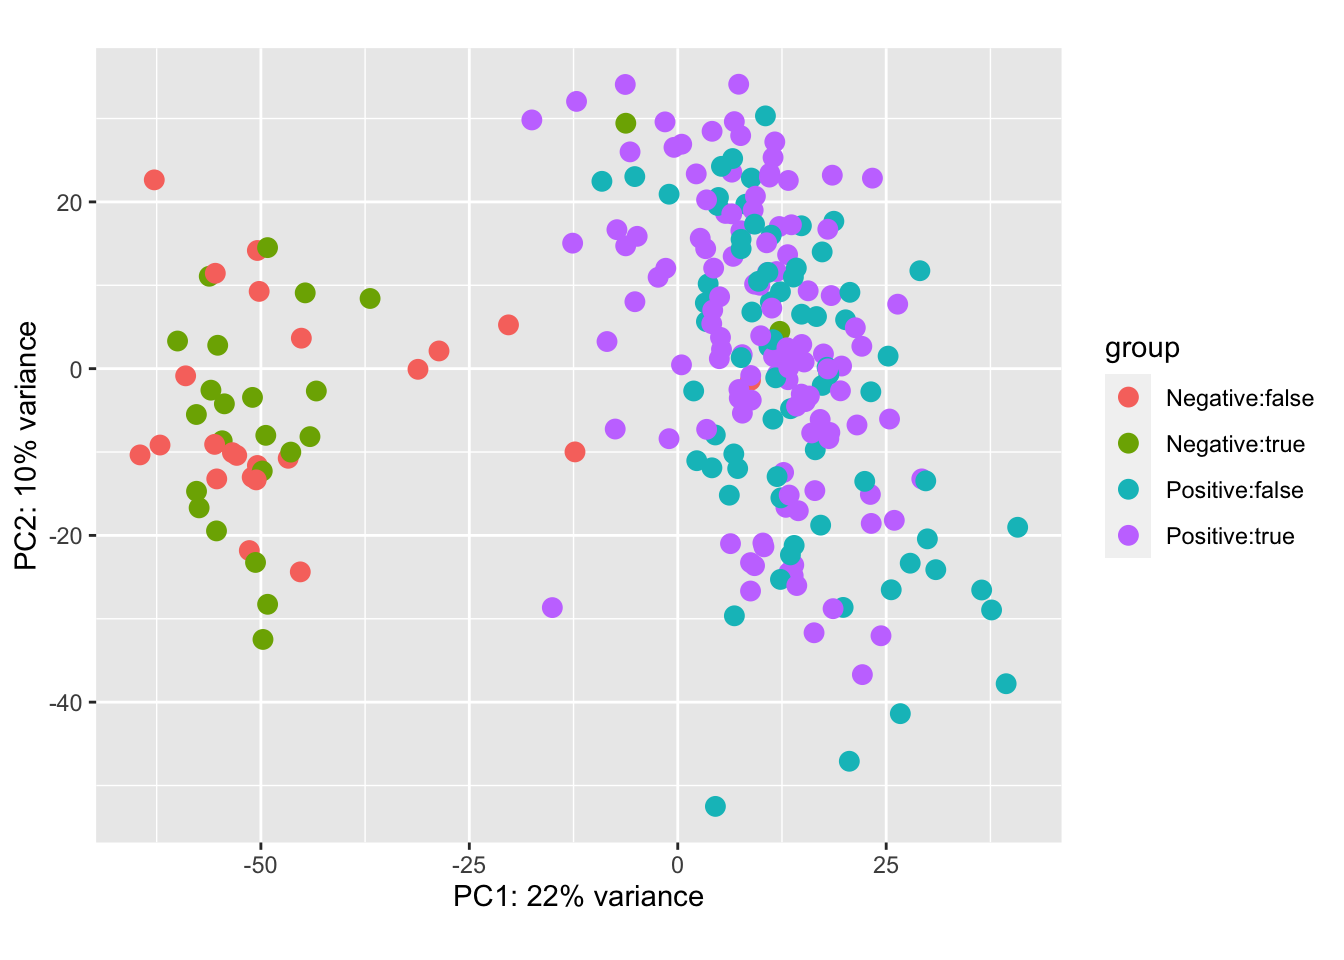
\includegraphics{RNAseq_DEGs_files/figure-latex/unnamed-chunk-15-1.pdf}

\subsection{Hierarchical Clustering}\label{hierarchical-clustering}

The \textbf{HC} plot shows that most of ER-negative cases are aggregated
together into a separate cluster. However, the separation is not perfect
and the \textbf{heatmap} is not very informative because of the large
number of irrelevant genes.

In this example we use \textbf{pheatmap} (pretty heatmap) package to
make the heatmap and to perform hierarchical clustering. Other often
used packages for plotting heatmaps include \textbf{heatmap} and
\textbf{heatmap.2}. \textbf{heatmap} is a reliable base-R tool; however
it lacks many convinience features. \textbf{heatmap.2} (from gplots
package) has a bug, which makes it very slow for plotting large matrices
(\textasciitilde{}28k genes x \textasciitilde{}230 samples is considered
to be a large matrix for this purpose). Also, the heatmap could be
plotted with \textbf{ggplot2}, which could provide many advantages
(e.g.~animation with \textbf{plotly}). I selected \textbf{pheatmap} here
because of its simplicity and convinience; and because this tutorial
does not need the advasnced \textbf{ggplot2} features.

Beware: calculating dendrogram for \textasciitilde{}28k hgenes may take
very long time and require large memory. The code includes
\textbf{cluster\_rows = FALSE} option in \textbf{pheatmap} to avoid the
long calculations.

\begin{Shaded}
\begin{Highlighting}[]
\CommentTok{# Libraries for drawing heatmap}
\CommentTok{#install.packages("RColorBrewer")}
\CommentTok{#install.packages("pheatmap")}
\KeywordTok{suppressWarnings}\NormalTok{(}\KeywordTok{suppressMessages}\NormalTok{(}\KeywordTok{library}\NormalTok{(RColorBrewer)))}
\KeywordTok{suppressWarnings}\NormalTok{(}\KeywordTok{suppressMessages}\NormalTok{(}\KeywordTok{library}\NormalTok{(pheatmap)))}

\CommentTok{# Matrix for clustering and heatmap}
\NormalTok{vst_counts <-}\StringTok{ }\KeywordTok{assay}\NormalTok{(vst_dds)}
\KeywordTok{dim}\NormalTok{(vst_counts)}

\CommentTok{# Scale and center by rows. }
\CommentTok{# Heatmap-making functions often include in-built functions for scaling.  }
\CommentTok{# However, this script does it manually to allow explicit centering, facilitating }
\CommentTok{# green-black-red palette, when black corresponds to zero (i.e. black = mean gene expression). }
\NormalTok{vst_counts <-}\StringTok{ }\KeywordTok{t}\NormalTok{(}\KeywordTok{scale}\NormalTok{(}\KeywordTok{t}\NormalTok{(vst_counts)))}

\CommentTok{# Make a dataframe with ER- and OCT- status}
\CommentTok{# (for colour-coded strips along the hea)}
\NormalTok{cases.df <-}\StringTok{ }\KeywordTok{as.data.frame}\NormalTok{(}\KeywordTok{colData}\NormalTok{(vst_dds))}
\NormalTok{cases.df <-}\StringTok{ }\NormalTok{cases.df }\OperatorTok\StringTok{ }\KeywordTok{select}\NormalTok{(oct, er)}

\CommentTok{# Make palette of 21 colours for heatmap drawing. }
\CommentTok{# The default heatmap palette would be white-yellow-red, }
\CommentTok{# which is not good for visualizing differences in genes expression. }
\NormalTok{gbr_}\DecValTok{21}\NormalTok{ <-}\StringTok{ }\KeywordTok{colorRampPalette}\NormalTok{(}\KeywordTok{c}\NormalTok{(}\StringTok{"green"}\NormalTok{, }\StringTok{"black"}\NormalTok{, }\StringTok{"red"}\NormalTok{))(}\DataTypeTok{n =} \DecValTok{21}\NormalTok{)}

\CommentTok{# Make breaks between colours}
\CommentTok{# By default, most hearmap-plotting tools place breaks at equal distance}
\CommentTok{# Customising breaks by placing them at quantiles makes the hearmap more informative}
\CommentTok{# (although this is a matter of personal preference :)}
\CommentTok{# The number of breaksshould be one more than the number of colours in palette}
\NormalTok{breaks_}\DecValTok{22}\NormalTok{ <-}\StringTok{ }\KeywordTok{quantile}\NormalTok{(vst_counts, }\DataTypeTok{probs=}\KeywordTok{seq}\NormalTok{(}\DecValTok{0}\NormalTok{,}\DecValTok{1}\NormalTok{,}\DataTypeTok{length.out=}\DecValTok{22}\NormalTok{))}

\CommentTok{# Make heatmap with dendrograms}
\CommentTok{# Calculating dendrogram for ~28k genes requires large memory and may crash a laptop}
\CommentTok{# On a laptop with 4 cores and 8GB RAM it may take ~30-40 min}
\CommentTok{# To suppress genes dendrogram add "cluster_rows = FALSE" option }
\KeywordTok{pheatmap}\NormalTok{(}
  \DataTypeTok{mat =}\NormalTok{ vst_counts, }\CommentTok{# matrix with data}
  \DataTypeTok{color =}\NormalTok{ gbr_}\DecValTok{21}\NormalTok{, }\CommentTok{# user-defined palette}
  \DataTypeTok{breaks =}\NormalTok{ breaks_}\DecValTok{22}\NormalTok{, }\CommentTok{# user-defined breaks between colours}
  \DataTypeTok{scale =} \StringTok{"none"}\NormalTok{, }\CommentTok{# has been scaled manually}
  \DataTypeTok{annotation_col =}\NormalTok{ cases.df, }\CommentTok{# data frame with ER- and OCT- status}
  \DataTypeTok{border_color =} \OtherTok{NA}\NormalTok{, }\CommentTok{# dont draw borders inside the heatmap}
  \DataTypeTok{cluster_rows =} \OtherTok{FALSE}\NormalTok{, }\CommentTok{# dont cluster genes (to avoid long calculations)}
  \DataTypeTok{show_colnames =} \OtherTok{FALSE}\NormalTok{, }\CommentTok{# too many samples names to show}
  \DataTypeTok{show_rownames =} \OtherTok{FALSE}\NormalTok{, }\CommentTok{# too many gene names to show}
  \DataTypeTok{main =} \StringTok{"HC with all genes (~28k)"}\NormalTok{)}

\CommentTok{# Clean-up}
\KeywordTok{rm}\NormalTok{(vst_counts, gbr_}\DecValTok{21}\NormalTok{, breaks_}\DecValTok{22}\NormalTok{, cases.df)}
\end{Highlighting}
\end{Shaded}

\textcolor{red}{Note that the figure shown below was generated without < cluster\_rows = FALSE > option, to illustrate the genes clustering.}

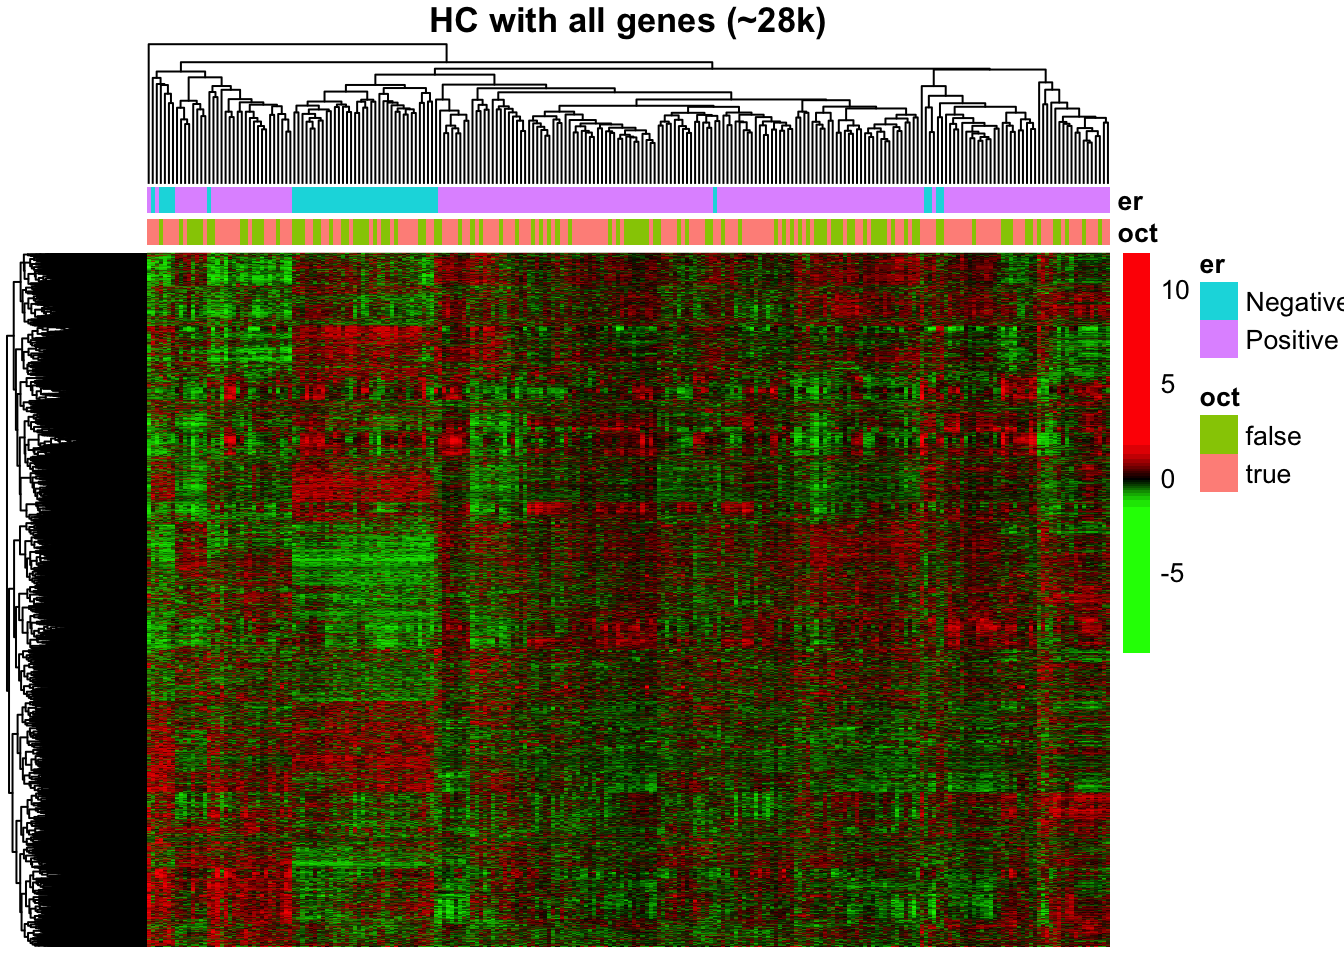
\includegraphics[width=1\linewidth]{/Users/alexey/OneDrive/Documents/Teaching/Lecturing/rna-seq-ebi-2020-tutorial/analysis/figures/f02_hc_28k}

\section{Calculating DEGs}\label{calculating-degs}

Overall, the preliminary exploration has suggested that ER-positive and
ER-negative tumours have \textbf{distinctive} gene expression profiles.
So, what are the specific Differentially Expressed Genes (DEGs)?

In practice, all the complicated DESeq2 statistics (discussed elsewere)
is hidden from the user within \textbf{a single function call}, which
adds the DEG results to the original DESeq2 dataset object \ldots{}

\begin{Shaded}
\begin{Highlighting}[]
\CommentTok{# Calculate the differentially expressed genes}
\NormalTok{ddx <-}\StringTok{ }\KeywordTok{DESeq}\NormalTok{(dds) }
\end{Highlighting}
\end{Shaded}

\begin{verbatim}
## estimating size factors
\end{verbatim}

\begin{verbatim}
## estimating dispersions
\end{verbatim}

\begin{verbatim}
## gene-wise dispersion estimates
\end{verbatim}

\begin{verbatim}
## mean-dispersion relationship
\end{verbatim}

\begin{verbatim}
## final dispersion estimates
\end{verbatim}

\begin{verbatim}
## fitting model and testing
\end{verbatim}

\begin{verbatim}
## -- replacing outliers and refitting for 2448 genes
## -- DESeq argument 'minReplicatesForReplace' = 7 
## -- original counts are preserved in counts(dds)
\end{verbatim}

\begin{verbatim}
## estimating dispersions
\end{verbatim}

\begin{verbatim}
## fitting model and testing
\end{verbatim}

\begin{Shaded}
\begin{Highlighting}[]
\CommentTok{# summary of the DESeq Dataset with added results}
\NormalTok{ddx }
\end{Highlighting}
\end{Shaded}

\begin{verbatim}
## class: DESeqDataSet 
## dim: 28362 238 
## metadata(1): version
## assays(6): counts mu ... replaceCounts replaceCooks
## rownames(28362): ENSG00000000003.13 ENSG00000000005.5 ... ENSG00000281912.1 ENSG00000281920.1
## rowData names(29): gene_id gene_name ... maxCooks replace
## colnames(238): TCGA-A7-A0DA TCGA-D8-A1XU ... TCGA-D8-A1XB TCGA-AO-A03M
## colData names(4): oct er sizeFactor replaceable
\end{verbatim}

\begin{Shaded}
\begin{Highlighting}[]
\CommentTok{# Clean-up}
\KeywordTok{rm}\NormalTok{(dds)}
\end{Highlighting}
\end{Shaded}

\section{Extracting results}\label{extracting-results}

The results of differential gene expression analysis have been added to
DESeq2 Data Set. The next chunk of code shows how to extract these
results. This tutorial only considers the \textbf{key results} of DESeq2
analysis. Look for more details in DESeq2 package documentation.

\subsection{Explore default
thresholds}\label{explore-default-thresholds}

For each gene DESeq2 provides mean expression, fold change and measures
of statistical significance (p and ``adjusted p'') that allow to
conclude whether this gene has been significantly changed.

The default DESeq's thersholds for labelling genes as ``significant''
are

\begin{itemize}
\tightlist
\item
  the null hypothesis asuming that there is no difference between the
  compared groups\\
\item
  FDR 0.1
\end{itemize}

These thersholds reflect the practices for RNA-seq experiments with a
small number of sampes (the most common case at the early time of
RNA-seq development).

In this tutorial, when the data includes more than two hundreed samples,
\textbf{the default DESeq's thresholds suggest that more than a half of
the genes are ``significantly'' changed} between ER-positive and
Triple-negative breast cancers (68\% = 32 Up-regilated and 36\%
Down-regulated genes). While it is well known that these cancers have
very strong biological differences, such high proportion of changed
genes is not realistic. It contradicts to a common assumption, that ony
a small proportion of genes should be significantly changed. Also, the
distribution of p-values shows noticeable inflation (increased
proportion of low p-values) comparatively to the uniform distribution,
typically expected under the null.

\begin{Shaded}
\begin{Highlighting}[]
\CommentTok{# Testing against H0 of no difference at FDR 0.1}
\NormalTok{DESeq2_any_change_fdr_}\FloatTok{0.1}\NormalTok{ <-}\StringTok{ }\KeywordTok{results}\NormalTok{(ddx)}
\NormalTok{DESeq2_any_change_fdr_}\FloatTok{0.1}
\end{Highlighting}
\end{Shaded}

\begin{verbatim}
## log2 fold change (MLE): er Positive vs Negative 
## Wald test p-value: er Positive vs Negative 
## DataFrame with 28362 rows and 6 columns
##                            baseMean     log2FoldChange              lfcSE              stat               pvalue                 padj
##                           <numeric>          <numeric>          <numeric>         <numeric>            <numeric>            <numeric>
## ENSG00000000003.13 3254.88256154068 -0.690175380631575  0.142786200450243 -4.83362802886601 1.34066988573307e-06  4.3852011647055e-06
## ENSG00000000005.5    56.40674633187   1.83304965161698  0.344713183710671  5.31760819787942 1.05140164399798e-07 3.96382472777758e-07
## ENSG00000000419.11 2311.61509753107 -0.373419784953396 0.0828390167004984 -4.50777664712611 6.55104842598776e-06 1.93502223971948e-05
## ENSG00000000457.12 2069.88515433684  0.376458293887623 0.0860125820091379  4.37678168814452 1.20444502953923e-05 3.42632597069124e-05
## ENSG00000000460.15 864.522147486874 -0.812238896522597  0.112023122992459 -7.25063607249438 4.14818894531819e-13 2.94864498413821e-12
## ...                             ...                ...                ...               ...                  ...                  ...
## ENSG00000281883.1  3.63933518666046 0.0230481676343476  0.217488426209903 0.105974226012851    0.915602801673173    0.934448602412902
## ENSG00000281896.1  53.2908748093281  0.268939774867321  0.152935139447986  1.75852178798182   0.0786587676712237    0.114055213123274
## ENSG00000281903.1  24.7506455382964  0.770290213483771  0.175801373989849  4.38159381807931 1.17814293010927e-05 3.35722794973969e-05
## ENSG00000281912.1   98.450301361596 -0.423446403741261  0.139085533004298 -3.04450358419502  0.00233064653179811  0.00461636964416915
## ENSG00000281920.1    5.641455151427   1.29108849263691  0.253834348705963  5.08634272398054 3.65034159677914e-07 1.29058823694652e-06
\end{verbatim}

\begin{Shaded}
\begin{Highlighting}[]
\CommentTok{# Explaing the columns in result table}
\KeywordTok{mcols}\NormalTok{(DESeq2_any_change_fdr_}\FloatTok{0.1}\NormalTok{, }\DataTypeTok{use.names =} \OtherTok{TRUE}\NormalTok{)}
\end{Highlighting}
\end{Shaded}

\begin{verbatim}
## DataFrame with 6 rows and 2 columns
##                        type                                     description
##                 <character>                                     <character>
## baseMean       intermediate       mean of normalized counts for all samples
## log2FoldChange      results log2 fold change (MLE): er Positive vs Negative
## lfcSE               results         standard error: er Positive vs Negative
## stat                results         Wald statistic: er Positive vs Negative
## pvalue              results      Wald test p-value: er Positive vs Negative
## padj                results                            BH adjusted p-values
\end{verbatim}

\begin{Shaded}
\begin{Highlighting}[]
\CommentTok{# A very high proportion of suggested DEGs}
\KeywordTok{summary}\NormalTok{(DESeq2_any_change_fdr_}\FloatTok{0.1}\NormalTok{)}
\end{Highlighting}
\end{Shaded}

\begin{verbatim}
## 
## out of 28362 with nonzero total read count
## adjusted p-value < 0.1
## LFC > 0 (up)       : 9053, 32%
## LFC < 0 (down)     : 10212, 36%
## outliers [1]       : 0, 0%
## low counts [2]     : 0, 0%
## (mean count < 0)
## [1] see 'cooksCutoff' argument of ?results
## [2] see 'independentFiltering' argument of ?results
\end{verbatim}

\begin{Shaded}
\begin{Highlighting}[]
\CommentTok{# Inflated p-values comparatively to the expected uniform distribution}
\KeywordTok{hist}\NormalTok{(DESeq2_any_change_fdr_}\FloatTok{0.1}\OperatorTok{$}\NormalTok{pvalue) }
\end{Highlighting}
\end{Shaded}

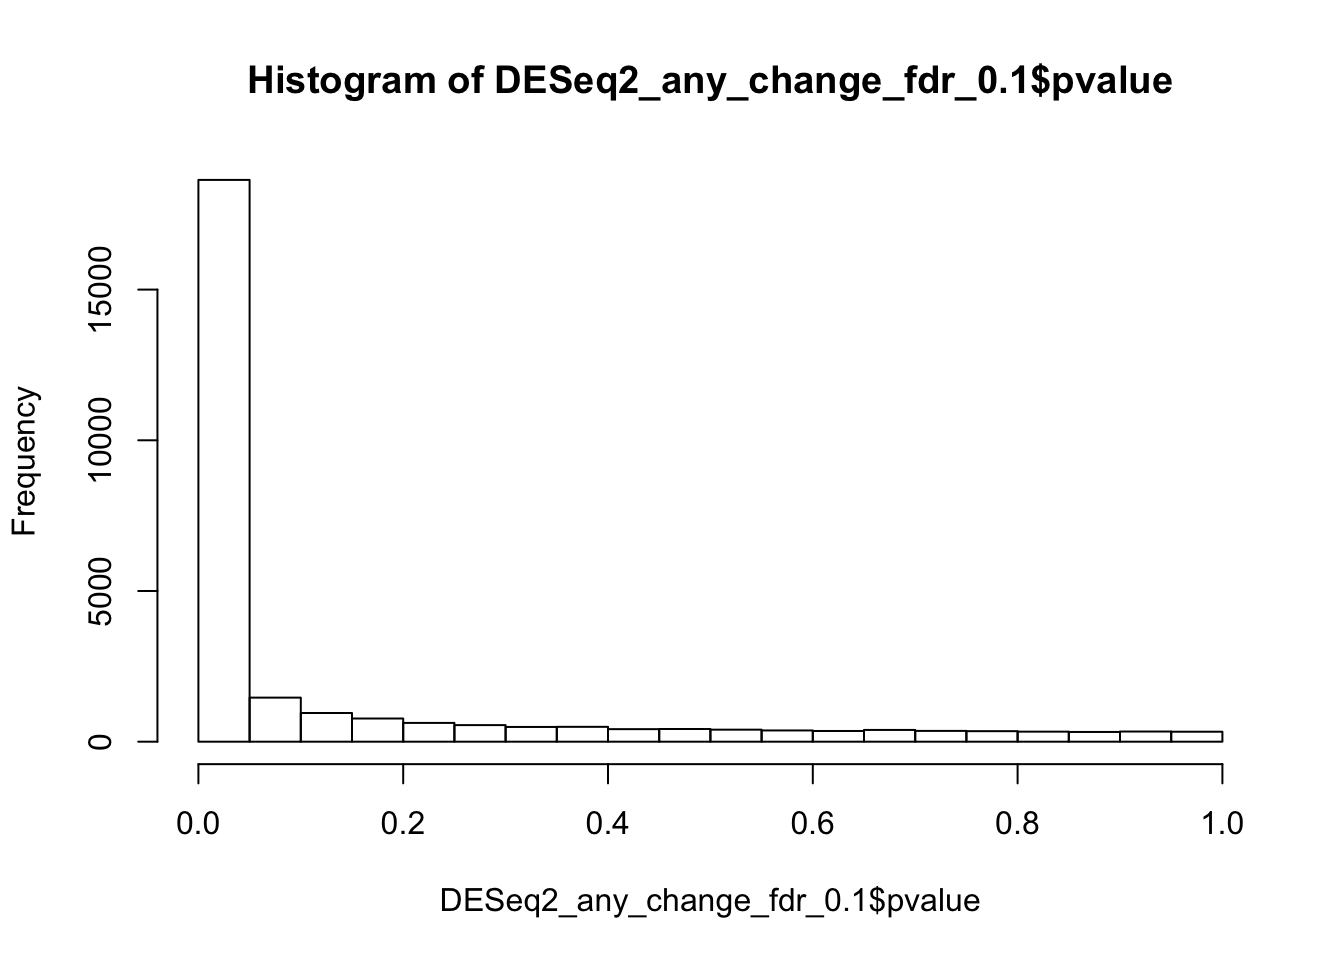
\includegraphics{RNAseq_DEGs_files/figure-latex/unnamed-chunk-19-1.pdf}

\subsection{User-defined thresholds}\label{user-defined-thresholds}

DESeq2 allows customised thresholds to select significant genes. The
following chunk of code shows how to select genes that are significant
for

\begin{itemize}
\tightlist
\item
  null hypothests that differences are less than 2-fold (log2 FC 1)\\
\item
  FDR 0.001
\end{itemize}

\textbf{The adjusted thresholds suggest less than 10\% are diferentially
expressed genes}: 3.9\% up-regulated and 4.8\% Down-regulated. This
looks much more realistic estimate, than the one suggested using the
default settings.

\begin{Shaded}
\begin{Highlighting}[]
\CommentTok{# Testing for at least 2-fold difference at FDR 0.001}
\NormalTok{DESeq2_fc_2_fdr_}\FloatTok{0.01}\NormalTok{ <-}\StringTok{ }\KeywordTok{results}\NormalTok{(ddx, }\DataTypeTok{lfcThreshold=}\DecValTok{1}\NormalTok{, }\DataTypeTok{alpha=}\FloatTok{0.01}\NormalTok{)}
\NormalTok{DESeq2_fc_2_fdr_}\FloatTok{0.01}
\end{Highlighting}
\end{Shaded}

\begin{verbatim}
## log2 fold change (MLE): er Positive vs Negative 
## Wald test p-value: er Positive vs Negative 
## DataFrame with 28362 rows and 6 columns
##                            baseMean     log2FoldChange              lfcSE             stat             pvalue              padj
##                           <numeric>          <numeric>          <numeric>        <numeric>          <numeric>         <numeric>
## ENSG00000000003.13 3254.88256154068 -0.690175380631575  0.142786200450243                0                  1                 1
## ENSG00000000005.5    56.40674633187   1.83304965161698  0.344713183710671 2.41664575357868 0.0156642534905646 0.135779204614729
## ENSG00000000419.11 2311.61509753107 -0.373419784953396 0.0828390167004984                0                  1                 1
## ENSG00000000457.12 2069.88515433684  0.376458293887623 0.0860125820091379                0                  1                 1
## ENSG00000000460.15 864.522147486874 -0.812238896522597  0.112023122992459                0                  1                 1
## ...                             ...                ...                ...              ...                ...               ...
## ENSG00000281883.1  3.63933518666046 0.0230481676343476  0.217488426209903                0                  1                 1
## ENSG00000281896.1  53.2908748093281  0.268939774867321  0.152935139447986                0                  1                 1
## ENSG00000281903.1  24.7506455382964  0.770290213483771  0.175801373989849                0                  1                 1
## ENSG00000281912.1   98.450301361596 -0.423446403741261  0.139085533004298                0                  1                 1
## ENSG00000281920.1    5.641455151427   1.29108849263691  0.253834348705963 1.14676557416627  0.251478520760158                 1
\end{verbatim}

\begin{Shaded}
\begin{Highlighting}[]
\CommentTok{# Check proportion of differentially expressed genes}
\KeywordTok{summary}\NormalTok{(DESeq2_fc_2_fdr_}\FloatTok{0.01}\NormalTok{)}
\end{Highlighting}
\end{Shaded}

\begin{verbatim}
## 
## out of 28362 with nonzero total read count
## adjusted p-value < 0.01
## LFC > 1.00 (up)    : 1118, 3.9%
## LFC < -1.00 (down) : 1358, 4.8%
## outliers [1]       : 0, 0%
## low counts [2]     : 0, 0%
## (mean count < 0)
## [1] see 'cooksCutoff' argument of ?results
## [2] see 'independentFiltering' argument of ?results
\end{verbatim}

\begin{Shaded}
\begin{Highlighting}[]
\CommentTok{# Distribution of p-values: }
\CommentTok{# not uniform, but without the huge inflation either  }
\KeywordTok{hist}\NormalTok{(DESeq2_fc_2_fdr_}\FloatTok{0.01}\OperatorTok{$}\NormalTok{pvalue)}
\end{Highlighting}
\end{Shaded}

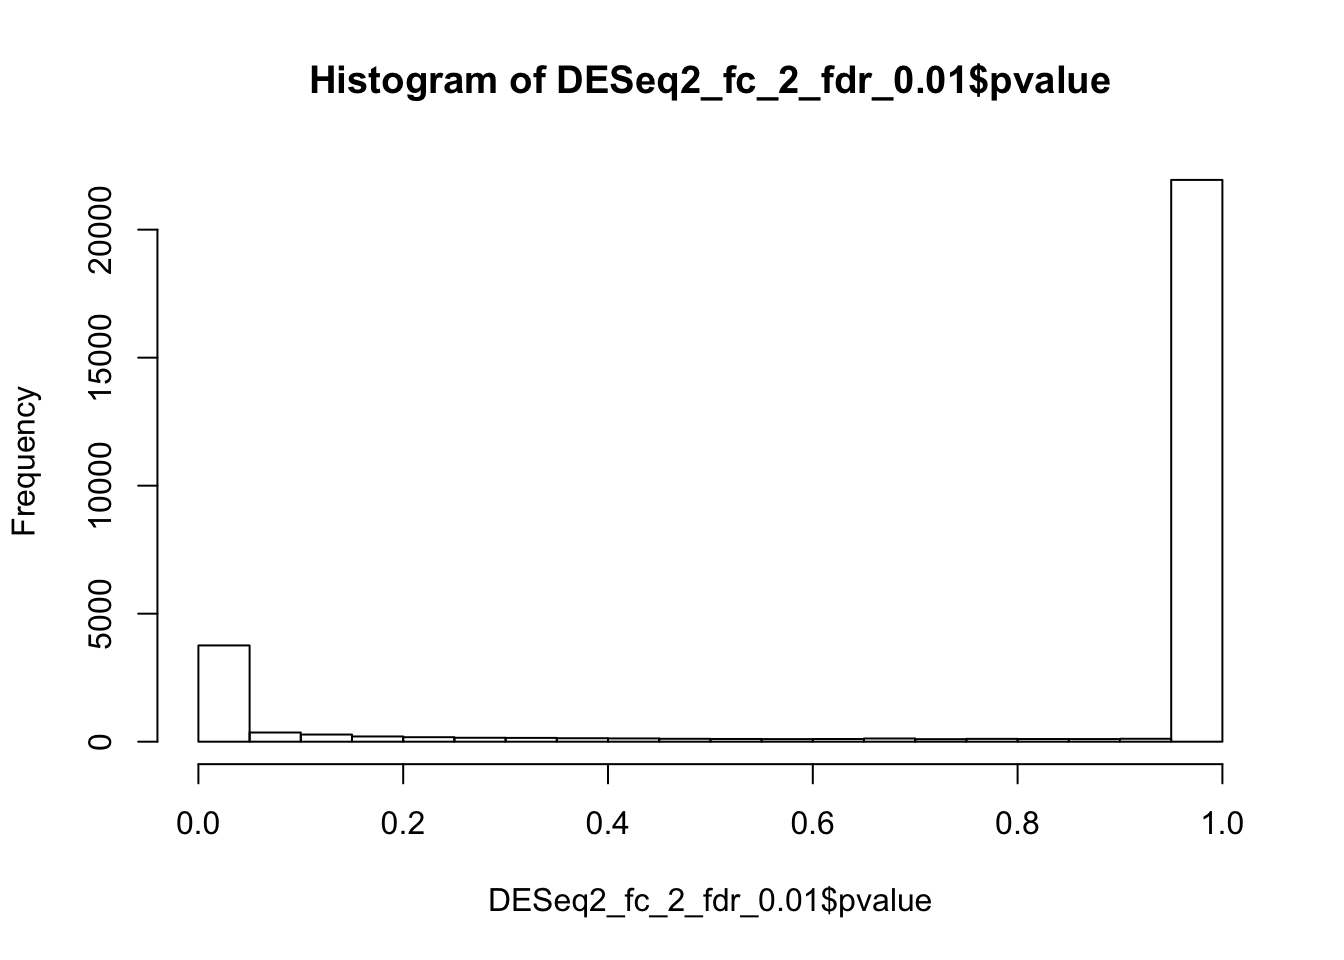
\includegraphics{RNAseq_DEGs_files/figure-latex/unnamed-chunk-20-1.pdf}

\subsection{Compare results with different
thresholds}\label{compare-results-with-different-thresholds}

Importantly, the above result with adjusted thresholds is NOT equivalent
to mere selecting of genes with fold change \textgreater{}2 from the
result obtained earlier using the default thersholds. While the
fold-change and mean expression, of course, remain the same, the
p-values and FDR have been changed, because they are calculated against
a different null hypothesis. See help for \textbf{DESEq2::results}
function for more details.

\begin{Shaded}
\begin{Highlighting}[]
\KeywordTok{plot}\NormalTok{(DESeq2_fc_2_fdr_}\FloatTok{0.01}\OperatorTok{$}\NormalTok{baseMean, DESeq2_any_change_fdr_}\FloatTok{0.1}\OperatorTok{$}\NormalTok{baseMean,}
     \DataTypeTok{main=}\StringTok{"Compare mean expressions"}\NormalTok{)}
\KeywordTok{abline}\NormalTok{(}\DecValTok{0}\NormalTok{,}\DecValTok{1}\NormalTok{, }\DataTypeTok{col=}\StringTok{"red"}\NormalTok{, }\DataTypeTok{lty=}\DecValTok{2}\NormalTok{)}
\end{Highlighting}
\end{Shaded}

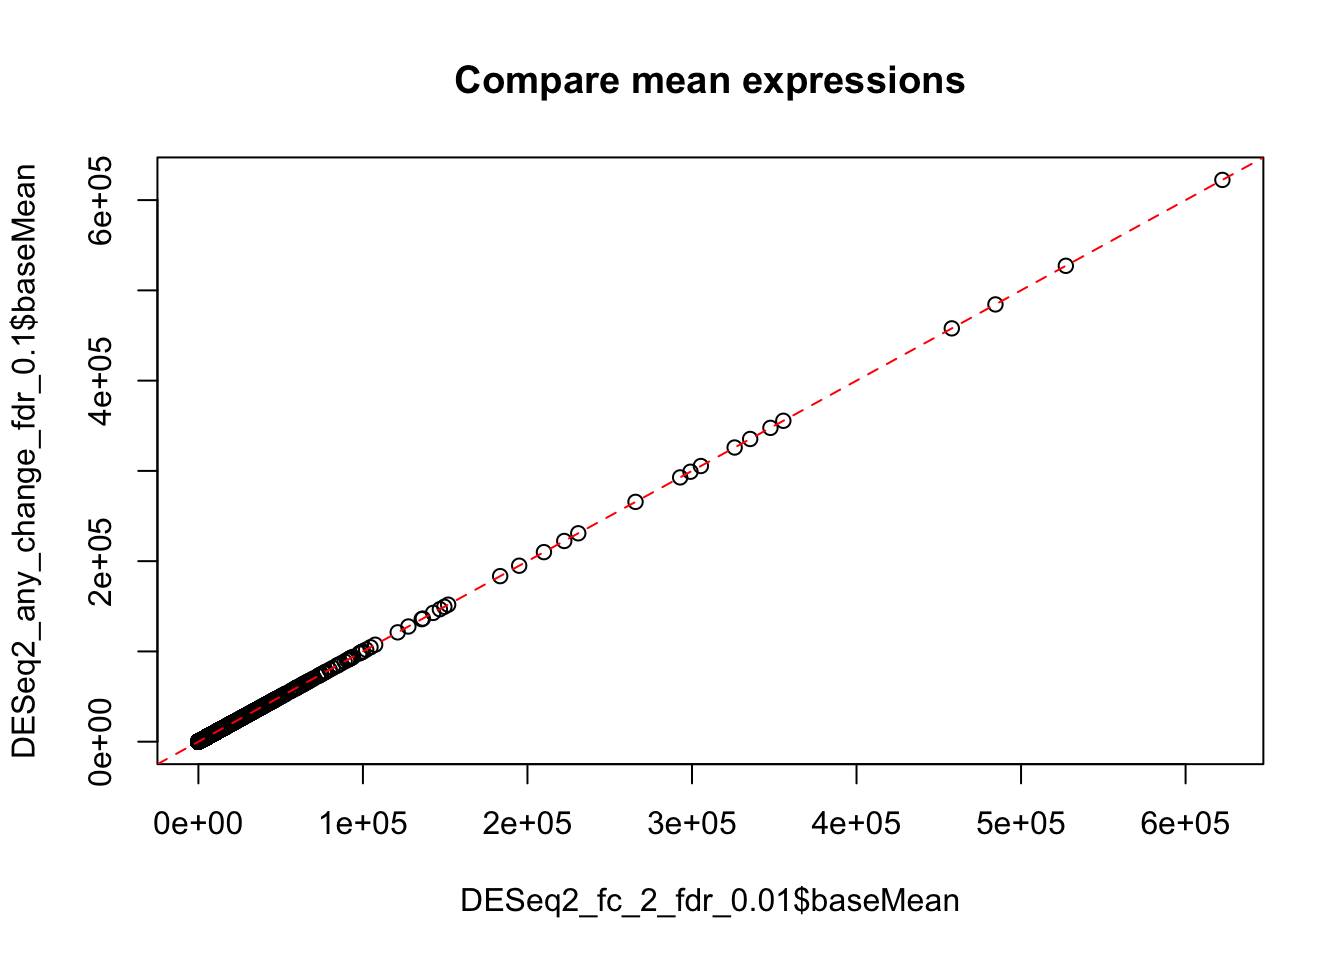
\includegraphics{RNAseq_DEGs_files/figure-latex/unnamed-chunk-21-1.pdf}

\begin{Shaded}
\begin{Highlighting}[]
\KeywordTok{plot}\NormalTok{(DESeq2_fc_2_fdr_}\FloatTok{0.01}\OperatorTok{$}\NormalTok{log2FoldChange, DESeq2_any_change_fdr_}\FloatTok{0.1}\OperatorTok{$}\NormalTok{log2FoldChange,}
     \DataTypeTok{main=}\StringTok{"Compare fold changes"}\NormalTok{)}
\KeywordTok{abline}\NormalTok{(}\DecValTok{0}\NormalTok{,}\DecValTok{1}\NormalTok{, }\DataTypeTok{col=}\StringTok{"red"}\NormalTok{, }\DataTypeTok{lty=}\DecValTok{2}\NormalTok{)}
\end{Highlighting}
\end{Shaded}

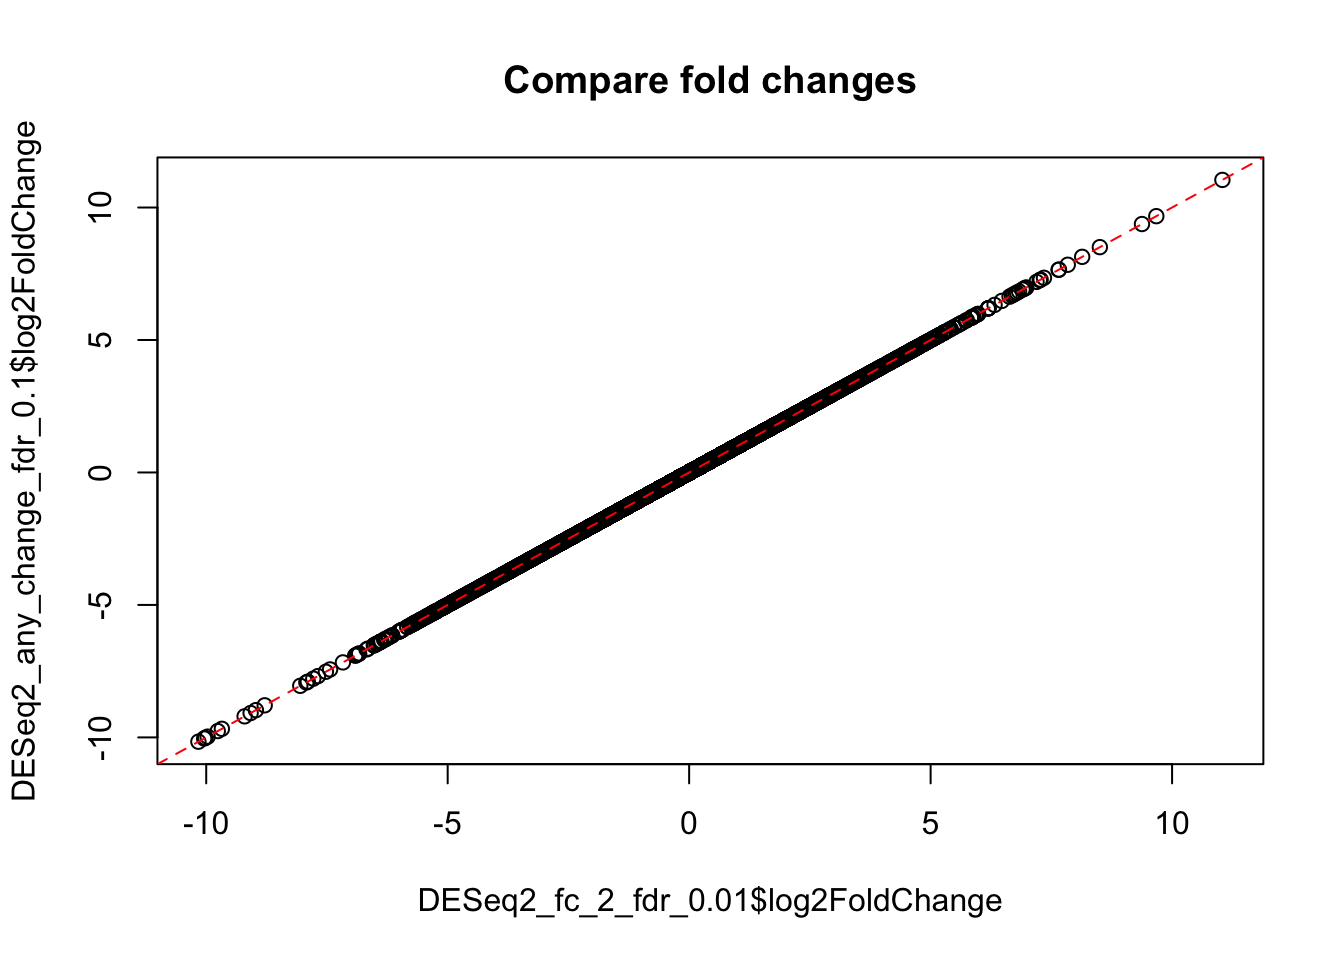
\includegraphics{RNAseq_DEGs_files/figure-latex/unnamed-chunk-21-2.pdf}

\begin{Shaded}
\begin{Highlighting}[]
\KeywordTok{plot}\NormalTok{(DESeq2_fc_2_fdr_}\FloatTok{0.01}\OperatorTok{$}\NormalTok{pvalue, DESeq2_any_change_fdr_}\FloatTok{0.1}\OperatorTok{$}\NormalTok{pvalue,}
     \DataTypeTok{main=}\StringTok{"Compare p-values"}\NormalTok{)}
\end{Highlighting}
\end{Shaded}

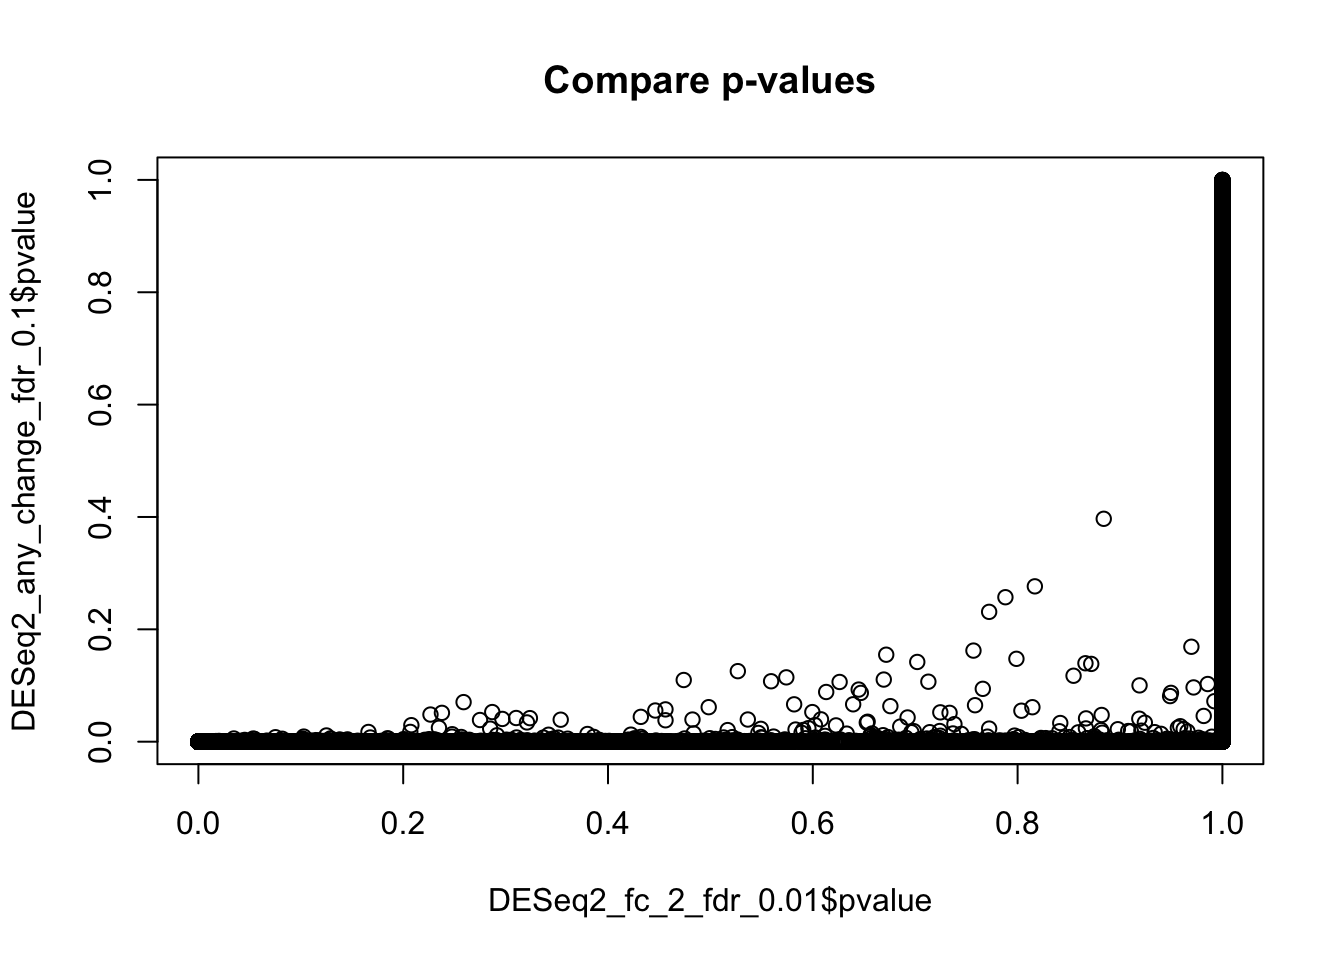
\includegraphics{RNAseq_DEGs_files/figure-latex/unnamed-chunk-21-3.pdf}

\section{Exploring results}\label{exploring-results}

In this tutorial, we will explore the results with the modifyed
thresholds: at least 2 fold change with FDR 0.01.

These thresholds where selected iteratively, checking the result against
a list of selcted known genes, which were reported previously by others
for ER-positive breast cancers.

\begin{Shaded}
\begin{Highlighting}[]
\KeywordTok{rm}\NormalTok{(DESeq2_any_change_fdr_}\FloatTok{0.1}\NormalTok{)}
\end{Highlighting}
\end{Shaded}

\subsection{Check genes with no
p-value}\label{check-genes-with-no-p-value}

Because of the large number of samples, no genes have been excluded from
analysis by DESeq in this example. However, for a smaller number of
samples, DESeq2 may exclude some genes, which are very unlikely to be
differentially expressed, to improve conditions for multiple testing
correction. For such genes the \textbf{padj} (FDR) value would be set to
\textbf{NA}.

\begin{Shaded}
\begin{Highlighting}[]
\KeywordTok{sum}\NormalTok{(}\KeywordTok{is.na}\NormalTok{(DESeq2_fc_2_fdr_}\FloatTok{0.01}\OperatorTok{$}\NormalTok{padj))}
\end{Highlighting}
\end{Shaded}

\begin{verbatim}
## [1] 0
\end{verbatim}

\subsection{Plot dispersions}\label{plot-dispersions}

Adjustment of dispersions is one of the key statistical tasks in DSEq2.
However, in this analysis, because of the large number of samples, the
dispersion adjustments were very modest (blue dots overlay the black
ones).

\begin{Shaded}
\begin{Highlighting}[]
\KeywordTok{plotDispEsts}\NormalTok{(ddx, }\DataTypeTok{main=}\StringTok{"Dispersion estimates and adjustments"}\NormalTok{)}
\end{Highlighting}
\end{Shaded}

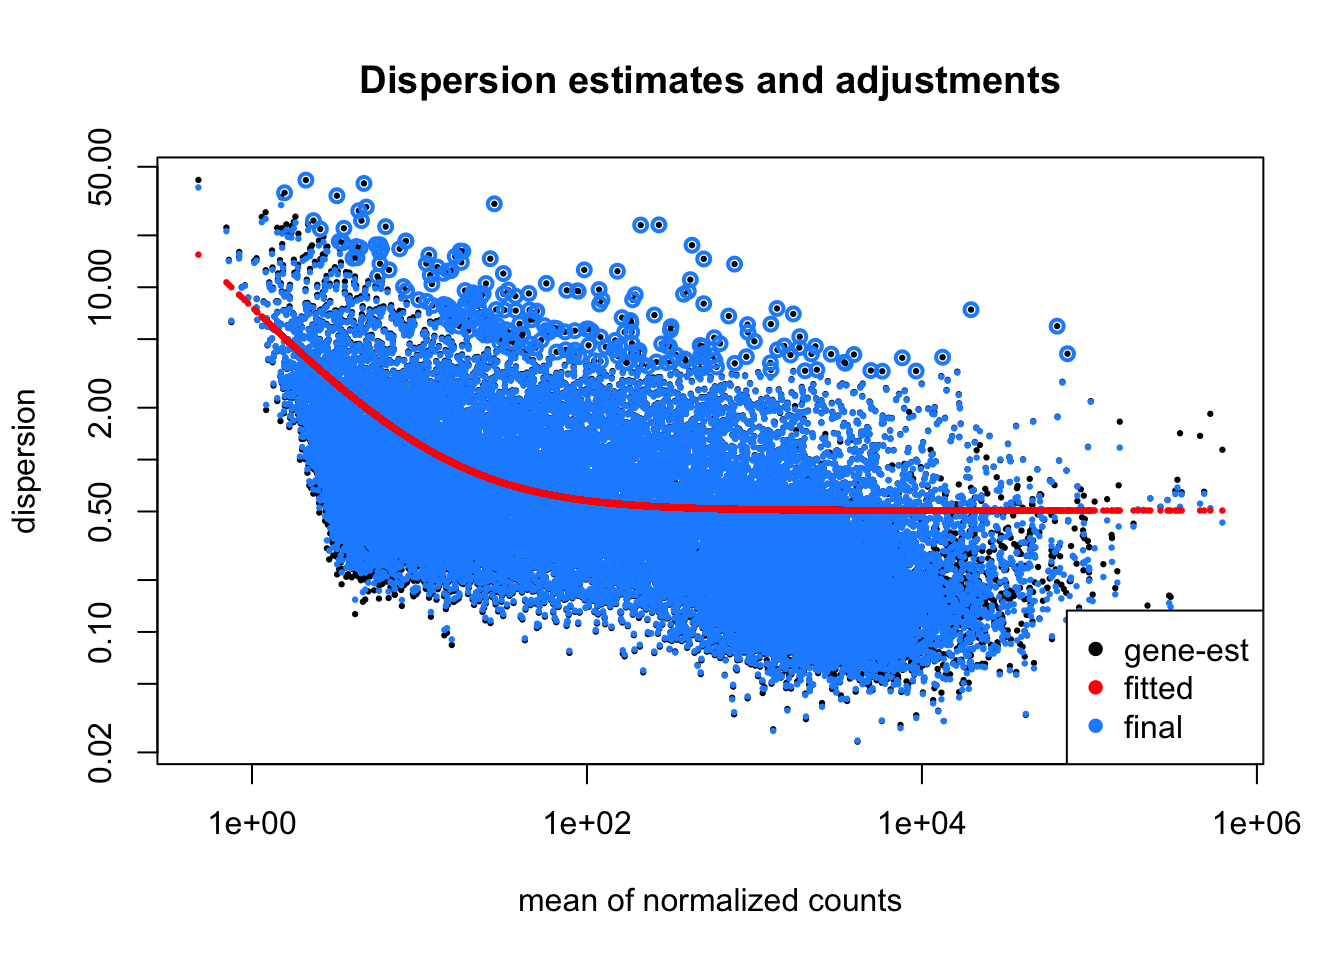
\includegraphics{RNAseq_DEGs_files/figure-latex/unnamed-chunk-24-1.pdf}

\subsection{MA plots}\label{ma-plots}

\textbf{MA plot} shows fold change along the y-axis, mean expression
along the x-axis and significance by colour coding (in red). Each dot
represents a gene. The genes equally expressed in both groups
(ER-positive and Triple-negative tumours) are located along the middle
zero-line. The differentially expressed genes will be located above- or
below- the zero-line.

Because of the large number of available samples, a large number of
genes have reached statistical ``significance'' at the default FDR
\textless{} 0.1 threshold (red dots). This is consistent with the strong
biological difference between ER-positive and ER-negative breast
cancers. A smaller, but still very large number of genes have reached
``significance'' at FDR \textless{} 10-6 level.

\begin{Shaded}
\begin{Highlighting}[]
\KeywordTok{plotMA}\NormalTok{(ddx, }\DataTypeTok{lfcThreshold=}\DecValTok{1}\NormalTok{, }\DataTypeTok{alpha=}\FloatTok{0.01}\NormalTok{, }\DataTypeTok{main=}\StringTok{"ER-pos vs Triple-neg}\CharTok{\textbackslash{}n}\StringTok{red: FC>2, FDR<0.01"}\NormalTok{)}
\end{Highlighting}
\end{Shaded}

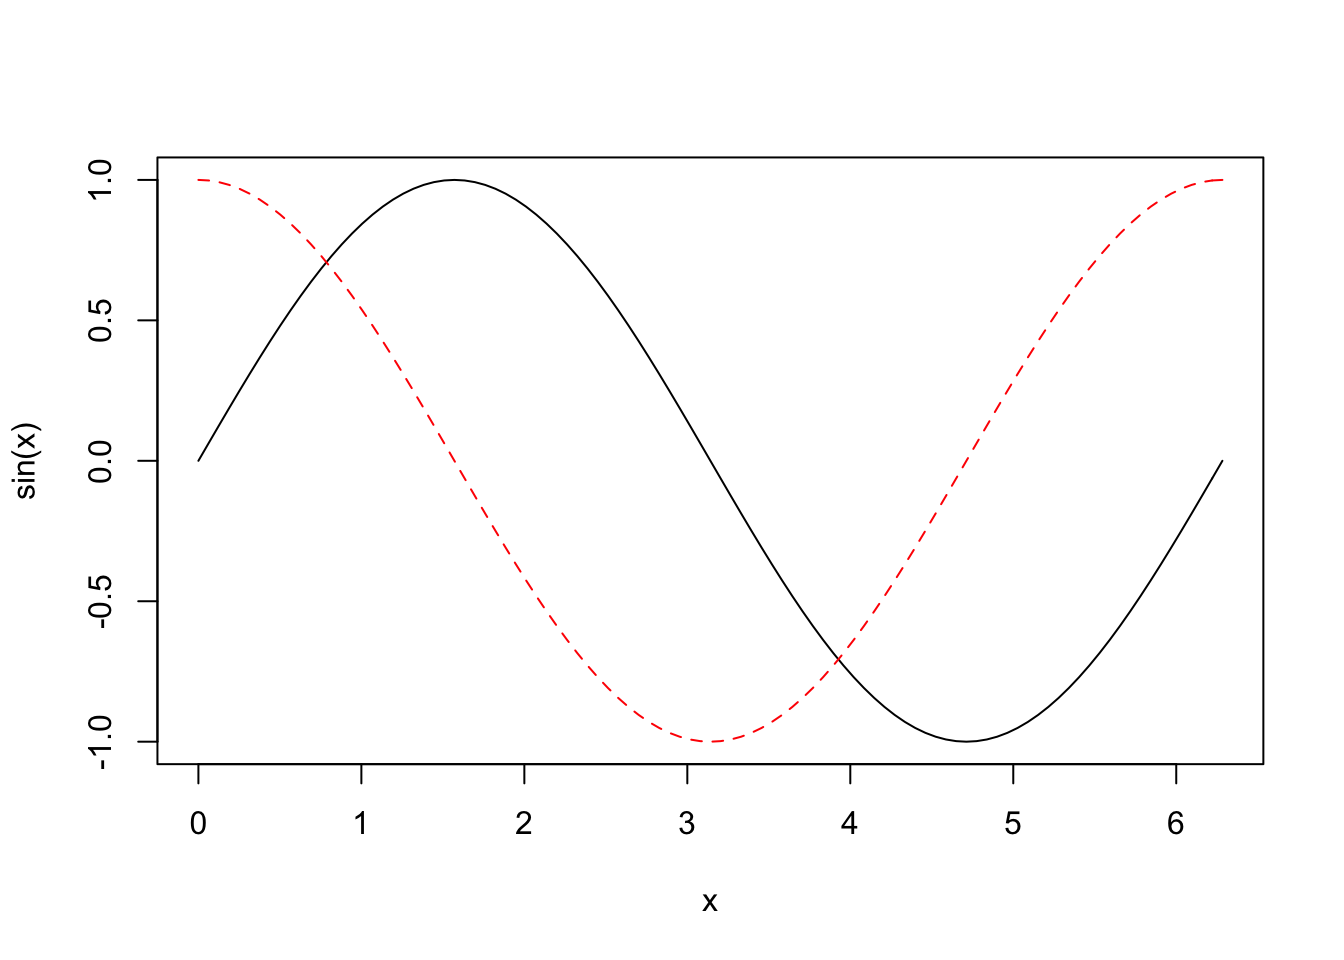
\includegraphics{RNAseq_DEGs_files/figure-latex/unnamed-chunk-25-1.pdf}

This would be the MA-plot for the \textbf{default} DESeq2 settings:

\begin{Shaded}
\begin{Highlighting}[]
\KeywordTok{plotMA}\NormalTok{(ddx, }\DataTypeTok{main=}\StringTok{"ER-pos vs Triple-neg}\CharTok{\textbackslash{}n}\StringTok{red: Any Change, FDR>0.1 (default settings)"}\NormalTok{)}
\end{Highlighting}
\end{Shaded}

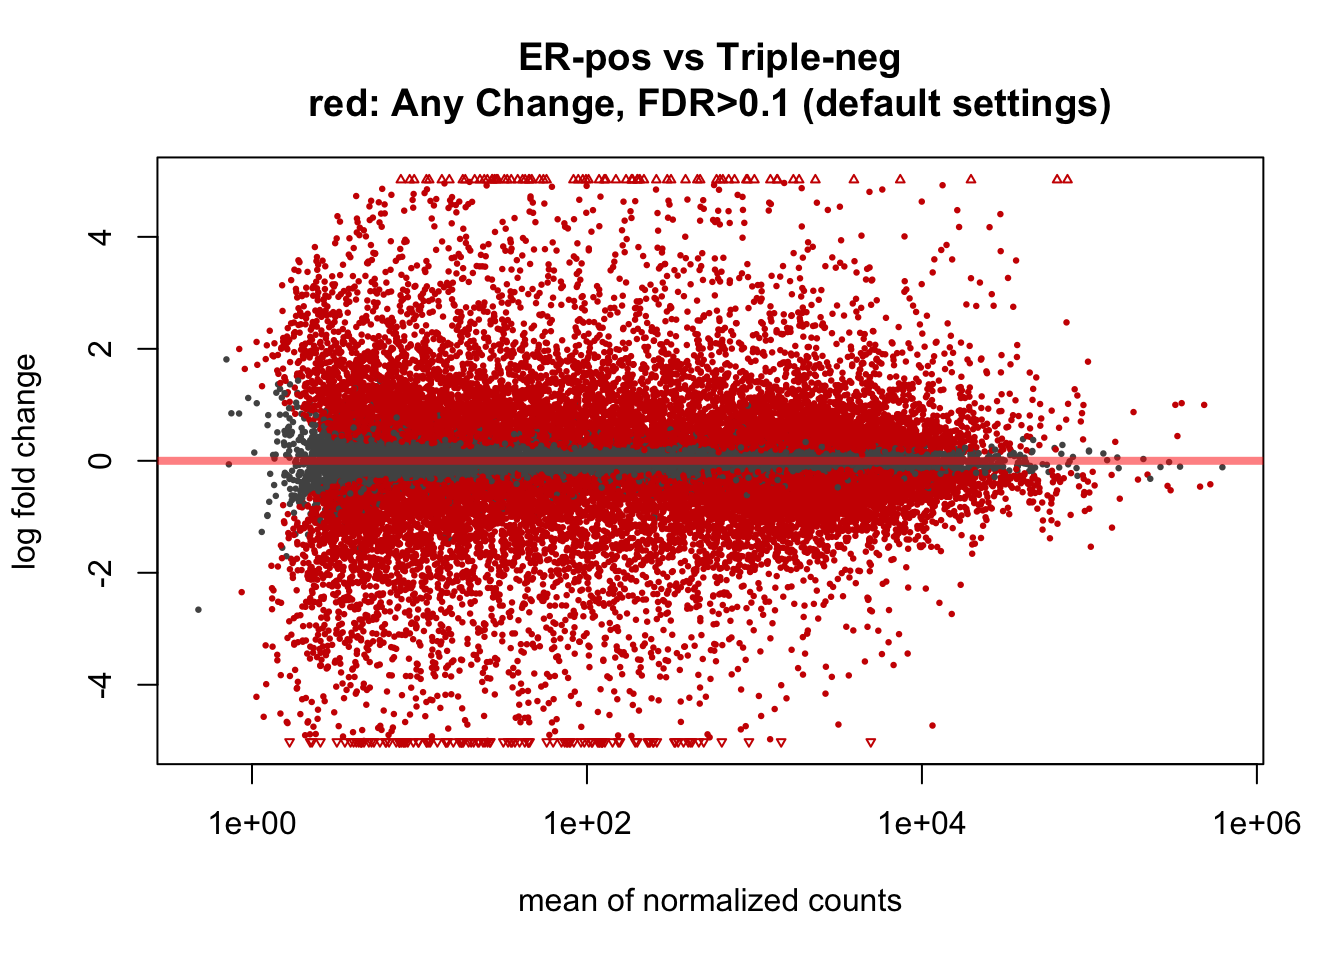
\includegraphics{RNAseq_DEGs_files/figure-latex/unnamed-chunk-26-1.pdf}

By default, of course, the null hypothesis is either of no difference,
or that the difference is below the specified logFC threshold. That
means the alternative hypothesis is that the changes are above the
threshold.

A very interesting and unusual feature of DESeq2 is that it allows to
test for alternative hypothesis that the change is \textbf{LESS} than a
specified threshold. In other words, DESeq2 provides \textbf{a
statistical framework to look for unchanged genes}:

\begin{Shaded}
\begin{Highlighting}[]
\KeywordTok{plotMA}\NormalTok{(ddx, }\DataTypeTok{lfcThreshold=}\DecValTok{1}\NormalTok{, }\DataTypeTok{altHypothesis=}\StringTok{"lessAbs"}\NormalTok{, }\DataTypeTok{alpha=}\FloatTok{0.01}\NormalTok{, }
       \DataTypeTok{main=}\StringTok{"ER-pos vs Triple-neg}\CharTok{\textbackslash{}n}\StringTok{red: FC<2, FDR<0.01"}\NormalTok{)}
\end{Highlighting}
\end{Shaded}

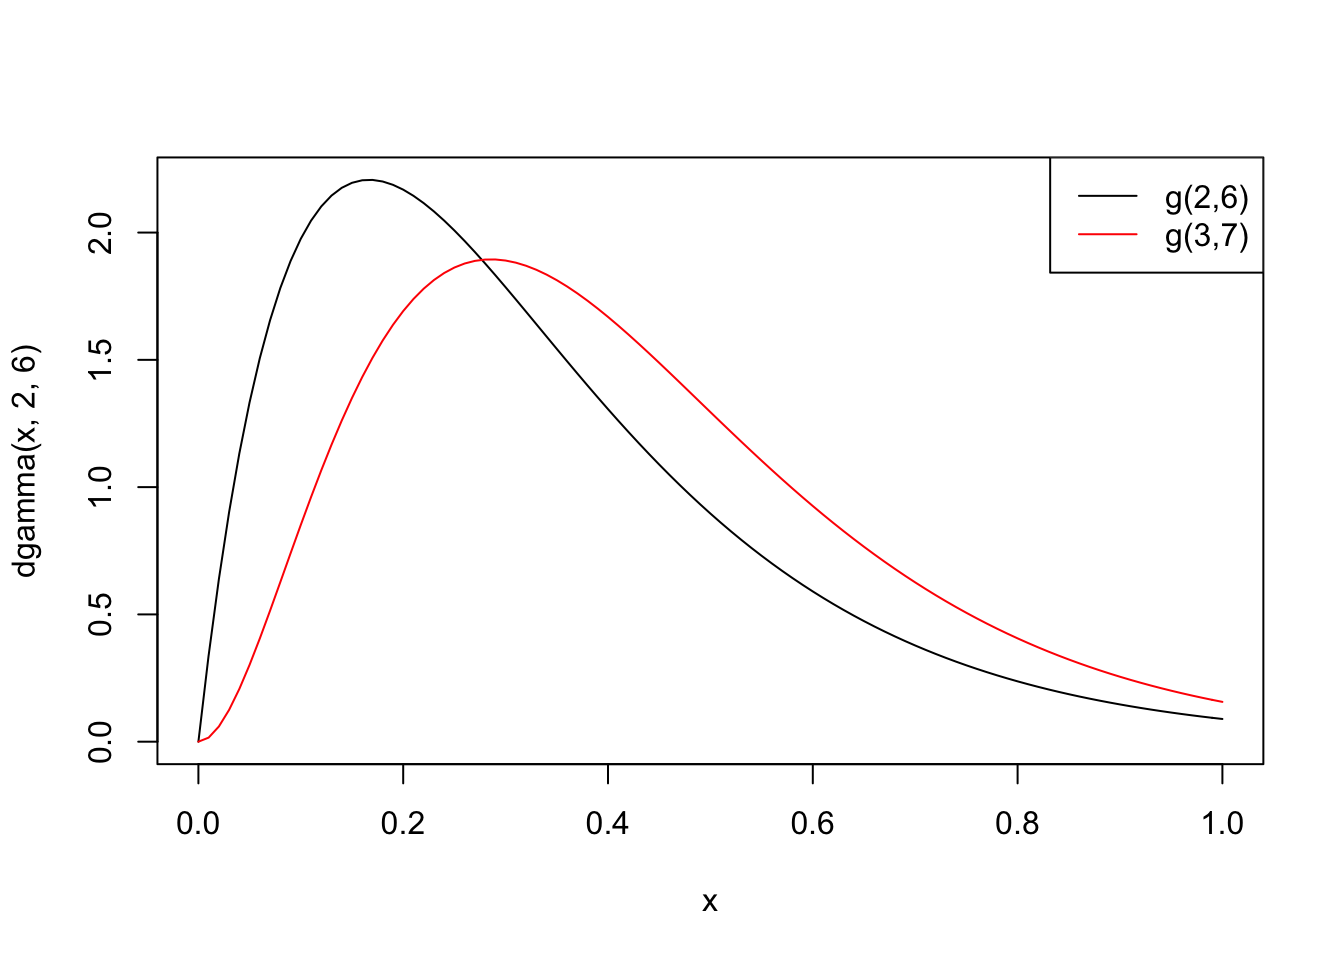
\includegraphics{RNAseq_DEGs_files/figure-latex/unnamed-chunk-27-1.pdf}

\subsection{Plot counts for an individual
gene}\label{plot-counts-for-an-individual-gene}

In this tutorial we will plot counts for Estrogen Receptor Alpha (ESR1)
comparing ER-positive and Triple-negative groups.

\begin{Shaded}
\begin{Highlighting}[]
\CommentTok{# Get gene ID for ESR1}
\NormalTok{ESR1_gene_id <-}\StringTok{ }\NormalTok{genes.df }\OperatorTok\StringTok{ }
\StringTok{  }\KeywordTok{filter}\NormalTok{(gene_name }\OperatorTok{==}\StringTok{ "ESR1"}\NormalTok{) }\OperatorTok\StringTok{ }
\StringTok{  }\KeywordTok{select}\NormalTok{(gene_id)}

\CommentTok{# Make the plot  }
\KeywordTok{plotCounts}\NormalTok{(ddx, }\DataTypeTok{gene=}\KeywordTok{as.character}\NormalTok{(ESR1_gene_id), }\DataTypeTok{intgroup =} \StringTok{"er"}\NormalTok{)}
\end{Highlighting}
\end{Shaded}

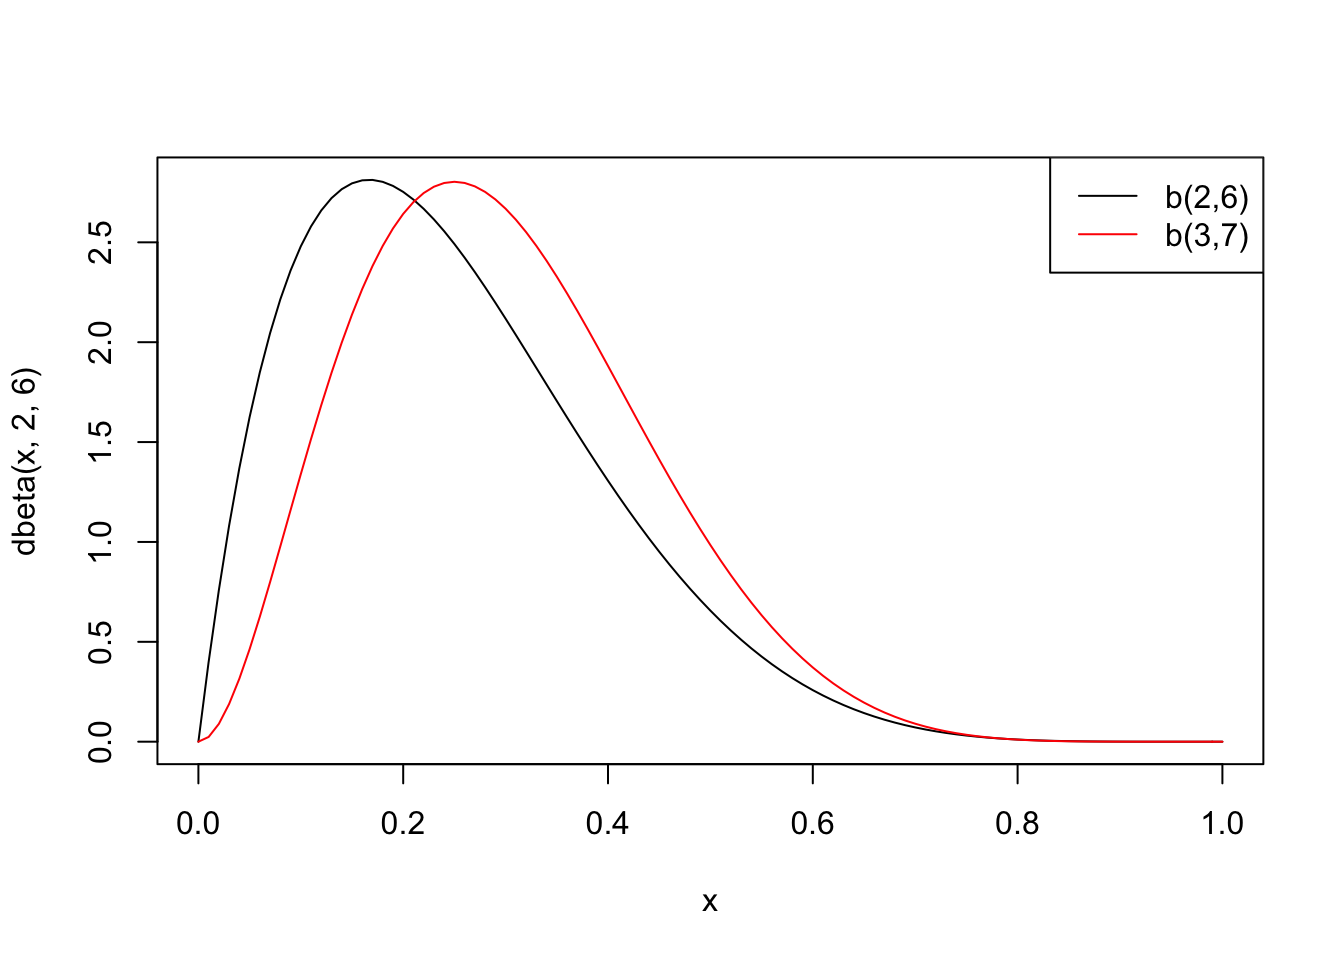
\includegraphics{RNAseq_DEGs_files/figure-latex/unnamed-chunk-28-1.pdf}

\begin{Shaded}
\begin{Highlighting}[]
\CommentTok{# Clean-up}
\KeywordTok{rm}\NormalTok{(ESR1_gene_id)}
\end{Highlighting}
\end{Shaded}

\subsection{Convert results to
data-frame}\label{convert-results-to-data-frame}

\begin{Shaded}
\begin{Highlighting}[]
\CommentTok{# The results can be converted to data.frame}
\NormalTok{DESeq2_fc_2_fdr_}\FloatTok{0.}\NormalTok{01_all_genes.df <-}\StringTok{ }\KeywordTok{as.data.frame}\NormalTok{(DESeq2_fc_2_fdr_}\FloatTok{0.01}\NormalTok{)}
\KeywordTok{head}\NormalTok{(DESeq2_fc_2_fdr_}\FloatTok{0.}\NormalTok{01_all_genes.df)}
\end{Highlighting}
\end{Shaded}

\begin{verbatim}
##                      baseMean log2FoldChange      lfcSE     stat     pvalue      padj
## ENSG00000000003.13 3254.88256     -0.6901754 0.14278620 0.000000 1.00000000 1.0000000
## ENSG00000000005.5    56.40675      1.8330497 0.34471318 2.416646 0.01566425 0.1357792
## ENSG00000000419.11 2311.61510     -0.3734198 0.08283902 0.000000 1.00000000 1.0000000
## ENSG00000000457.12 2069.88515      0.3764583 0.08601258 0.000000 1.00000000 1.0000000
## ENSG00000000460.15  864.52215     -0.8122389 0.11202312 0.000000 1.00000000 1.0000000
## ENSG00000000938.11  621.25238     -0.1733090 0.14869825 0.000000 1.00000000 1.0000000
\end{verbatim}

\begin{Shaded}
\begin{Highlighting}[]
\CommentTok{# Copy gene ID-s from the rownames to a column}
\NormalTok{DESeq2_fc_2_fdr_}\FloatTok{0.}\NormalTok{01_all_genes.df}\OperatorTok{$}\NormalTok{gene_id=}\KeywordTok{rownames}\NormalTok{(DESeq2_fc_2_fdr_}\FloatTok{0.}\NormalTok{01_all_genes.df)}
\KeywordTok{head}\NormalTok{(DESeq2_fc_2_fdr_}\FloatTok{0.}\NormalTok{01_all_genes.df)}
\end{Highlighting}
\end{Shaded}

\begin{verbatim}
##                      baseMean log2FoldChange      lfcSE     stat     pvalue      padj            gene_id
## ENSG00000000003.13 3254.88256     -0.6901754 0.14278620 0.000000 1.00000000 1.0000000 ENSG00000000003.13
## ENSG00000000005.5    56.40675      1.8330497 0.34471318 2.416646 0.01566425 0.1357792  ENSG00000000005.5
## ENSG00000000419.11 2311.61510     -0.3734198 0.08283902 0.000000 1.00000000 1.0000000 ENSG00000000419.11
## ENSG00000000457.12 2069.88515      0.3764583 0.08601258 0.000000 1.00000000 1.0000000 ENSG00000000457.12
## ENSG00000000460.15  864.52215     -0.8122389 0.11202312 0.000000 1.00000000 1.0000000 ENSG00000000460.15
## ENSG00000000938.11  621.25238     -0.1733090 0.14869825 0.000000 1.00000000 1.0000000 ENSG00000000938.11
\end{verbatim}

\begin{Shaded}
\begin{Highlighting}[]
\CommentTok{# Add gene names (using information obtained from the GTF file earlier)}
\NormalTok{DESeq2_fc_2_fdr_}\FloatTok{0.}\NormalTok{01_all_genes.df <-}\KeywordTok{left_join}\NormalTok{(DESeq2_fc_2_fdr_}\FloatTok{0.}\NormalTok{01_all_genes.df, genes.df, }\DataTypeTok{by=}\StringTok{"gene_id"}\NormalTok{)}
\KeywordTok{head}\NormalTok{(DESeq2_fc_2_fdr_}\FloatTok{0.}\NormalTok{01_all_genes.df)}
\end{Highlighting}
\end{Shaded}

\begin{verbatim}
##     baseMean log2FoldChange      lfcSE     stat     pvalue      padj            gene_id gene_name
## 1 3254.88256     -0.6901754 0.14278620 0.000000 1.00000000 1.0000000 ENSG00000000003.13    TSPAN6
## 2   56.40675      1.8330497 0.34471318 2.416646 0.01566425 0.1357792  ENSG00000000005.5      TNMD
## 3 2311.61510     -0.3734198 0.08283902 0.000000 1.00000000 1.0000000 ENSG00000000419.11      DPM1
## 4 2069.88515      0.3764583 0.08601258 0.000000 1.00000000 1.0000000 ENSG00000000457.12     SCYL3
## 5  864.52215     -0.8122389 0.11202312 0.000000 1.00000000 1.0000000 ENSG00000000460.15  C1orf112
## 6  621.25238     -0.1733090 0.14869825 0.000000 1.00000000 1.0000000 ENSG00000000938.11       FGR
\end{verbatim}

\begin{Shaded}
\begin{Highlighting}[]
\KeywordTok{dim}\NormalTok{(DESeq2_fc_2_fdr_}\FloatTok{0.}\NormalTok{01_all_genes.df)}
\end{Highlighting}
\end{Shaded}

\begin{verbatim}
## [1] 28362     8
\end{verbatim}

Make a separate dataframe with the differentially expressed genes only:
expression change at least 2-fold with FDR 0.01

\begin{Shaded}
\begin{Highlighting}[]
\CommentTok{# Select Differentially Expressed Genes only}
\NormalTok{DESeq2_fc_2_fdr_}\FloatTok{0.}\NormalTok{01_DEGs.df <-}\StringTok{ }\NormalTok{DESeq2_fc_2_fdr_}\FloatTok{0.}\NormalTok{01_all_genes.df }\OperatorTok\StringTok{ }
\StringTok{  }\KeywordTok{filter}\NormalTok{(}\OperatorTok{-}\KeywordTok{log10}\NormalTok{(padj) }\OperatorTok{>}\StringTok{ }\DecValTok{2}\NormalTok{, }\KeywordTok{abs}\NormalTok{(log2FoldChange) }\OperatorTok{>}\StringTok{ }\DecValTok{1}\NormalTok{) }\OperatorTok\StringTok{ }
\StringTok{  }\KeywordTok{select}\NormalTok{(gene_name, gene_id, baseMean, log2FoldChange, padj) }\OperatorTok\StringTok{ }
\StringTok{  }\KeywordTok{arrange}\NormalTok{(}\KeywordTok{desc}\NormalTok{(log2FoldChange))}

\CommentTok{# Check results}
\KeywordTok{dim}\NormalTok{(DESeq2_fc_2_fdr_}\FloatTok{0.}\NormalTok{01_DEGs.df)}
\end{Highlighting}
\end{Shaded}

\begin{verbatim}
## [1] 2476    5
\end{verbatim}

\begin{Shaded}
\begin{Highlighting}[]
\KeywordTok{head}\NormalTok{(DESeq2_fc_2_fdr_}\FloatTok{0.}\NormalTok{01_DEGs.df)}
\end{Highlighting}
\end{Shaded}

\begin{verbatim}
##       gene_name            gene_id   baseMean log2FoldChange         padj
## 1        CARTPT  ENSG00000164326.4   760.7236      11.041924 5.602005e-26
## 2          CPB1 ENSG00000153002.10 64177.1952       9.673386 3.075352e-48
## 3  RP11-53O19.2  ENSG00000248779.1   301.5455       9.376603 3.960013e-46
## 4 RP11-473L15.3  ENSG00000249203.1   171.1401       8.504287 3.198874e-43
## 5  RP11-680B3.2  ENSG00000240521.1   118.1529       8.138256 6.406333e-18
## 6        CLEC3A  ENSG00000166509.9 19635.8020       7.839747 2.696858e-24
\end{verbatim}

\begin{Shaded}
\begin{Highlighting}[]
\CommentTok{# Clean-up}
\KeywordTok{rm}\NormalTok{(DESeq2_fc_2_fdr_}\FloatTok{0.01}\NormalTok{)}
\end{Highlighting}
\end{Shaded}

\subsection{Check known genes}\label{check-known-genes}

The list of genes up-regulated in ER-positive breast cancers is not yet
definitevely established. Numerous papers report different lists of
genes in cell lines or clinical biopsies, using different study designs,
experimental methods etc. ESR1, PGR, TFF1, TFF3, FOXA1, GATA3 are
amongst the most consistently mentioned genes up-regulated in
ER-positive cancers. Reports about the genes down-regulated in
ER-positive breast cancers are even less consistent, although FOXC1, MIA
had been mentioned earlier in this context.

The changes in expression of selected known ER-associated genes confirm
that our findings are considtent with previous reports. In additon, our
analysis suggests many other genes, not yet reported in context of ER
signalling in breast cancer. The newly reported genes need to be
validated in an independent dataset before making definitive
conclusions.

\begin{Shaded}
\begin{Highlighting}[]
\CommentTok{# Make a list of selected previously known genes of interest}
\NormalTok{selected_known_genes=}\KeywordTok{c}\NormalTok{(}\StringTok{"ESR1"}\NormalTok{, }\StringTok{"PGR"}\NormalTok{, }\StringTok{"TFF1"}\NormalTok{, }\StringTok{"TFF3"}\NormalTok{, }\StringTok{"GATA3"}\NormalTok{, }\StringTok{"FOXA1"}\NormalTok{, }\StringTok{"FOXC1"}\NormalTok{, }\StringTok{"MIA"}\NormalTok{)}

\CommentTok{# Look at the genes of interest in the top DEGs in our dataset  }
\NormalTok{DESeq2_fc_2_fdr_}\FloatTok{0.}\NormalTok{01_DEGs.df }\OperatorTok\StringTok{ }
\StringTok{  }\KeywordTok{filter}\NormalTok{(gene_name }\OperatorTok\StringTok{ }\NormalTok{selected_known_genes)}
\end{Highlighting}
\end{Shaded}

\begin{verbatim}
##   gene_name            gene_id   baseMean log2FoldChange         padj
## 1      TFF1  ENSG00000160182.2 16259.9568       4.476394 9.765610e-15
## 2      ESR1 ENSG00000091831.20 29402.2500       4.406085 3.070201e-44
## 3      TFF3 ENSG00000160180.15 16669.3405       4.175744 1.344767e-18
## 4       PGR ENSG00000082175.13 11860.4295       3.597820 2.272716e-14
## 5     FOXA1  ENSG00000129514.5 18425.8831       2.792643 8.023961e-16
## 6     GATA3 ENSG00000107485.14 35098.3567       2.750493 1.204231e-22
## 7     FOXC1  ENSG00000054598.6  1822.2110      -3.702730 2.674219e-47
## 8       MIA  ENSG00000261857.5   296.8554      -3.865913 3.768407e-17
\end{verbatim}

\begin{Shaded}
\begin{Highlighting}[]
\CommentTok{# Clean-up}
\KeywordTok{rm}\NormalTok{(selected_known_genes)}
\end{Highlighting}
\end{Shaded}

\subsection{Volcano plot}\label{volcano-plot}

A \textbf{volcano plot} allows simultaneous visualisation of
significance (y axis) and fold change (x axis).

\begin{Shaded}
\begin{Highlighting}[]
\CommentTok{# Prepare colour-coding for genes: highlit the DEGs in red}
\NormalTok{genes_color <-}\StringTok{ }\KeywordTok{rep}\NormalTok{(}\StringTok{"blue"}\NormalTok{,}\KeywordTok{nrow}\NormalTok{(DESeq2_fc_2_fdr_}\FloatTok{0.}\NormalTok{01_all_genes.df))}
\StringTok{"red"}\NormalTok{ ->}\StringTok{ }\NormalTok{genes_color[DESeq2_fc_2_fdr_}\FloatTok{0.}\NormalTok{01_all_genes.df}\OperatorTok{$}\NormalTok{gene_id }\OperatorTok\StringTok{ }\NormalTok{DESeq2_fc_2_fdr_}\FloatTok{0.}\NormalTok{01_DEGs.df}\OperatorTok{$}\NormalTok{gene_id]}

\CommentTok{# Make plot}
\KeywordTok{plot}\NormalTok{(}\DataTypeTok{x=}\NormalTok{DESeq2_fc_2_fdr_}\FloatTok{0.}\NormalTok{01_all_genes.df}\OperatorTok{$}\NormalTok{log2FoldChange, }
     \DataTypeTok{y=}\OperatorTok{-}\KeywordTok{log10}\NormalTok{(DESeq2_fc_2_fdr_}\FloatTok{0.}\NormalTok{01_all_genes.df}\OperatorTok{$}\NormalTok{padj),}
     \DataTypeTok{col=}\NormalTok{genes_color, }
     \DataTypeTok{main=}\StringTok{"TCGA BTCA: ER-pos vs Triple-neg}\CharTok{\textbackslash{}n}\StringTok{FC 2, FDR 0.01"}\NormalTok{)}

\CommentTok{# Add lines to show thresholds for the top genes}
\KeywordTok{abline}\NormalTok{(}\DataTypeTok{h=}\DecValTok{2}\NormalTok{, }\DataTypeTok{lty=}\DecValTok{2}\NormalTok{) }\CommentTok{# FDR 0.01}
\KeywordTok{abline}\NormalTok{(}\DataTypeTok{v=}\OperatorTok{-}\DecValTok{1}\NormalTok{, }\DataTypeTok{lty=}\DecValTok{2}\NormalTok{) }\CommentTok{# FC < -2}
\KeywordTok{abline}\NormalTok{(}\DataTypeTok{v=}\DecValTok{1}\NormalTok{, }\DataTypeTok{lty=}\DecValTok{2}\NormalTok{) }\CommentTok{# FC > 2}

\CommentTok{# Label Estrogen Receptor Alpha gene}
\NormalTok{esr1.df <-}\StringTok{ }\NormalTok{DESeq2_fc_2_fdr_}\FloatTok{0.}\NormalTok{01_all_genes.df }\OperatorTok\StringTok{ }\KeywordTok{filter}\NormalTok{(gene_name }\OperatorTok{==}\StringTok{ "ESR1"}\NormalTok{)}
\KeywordTok{text}\NormalTok{(esr1.df}\OperatorTok{$}\NormalTok{log2FoldChange, }\OperatorTok{-}\KeywordTok{log10}\NormalTok{(esr1.df}\OperatorTok{$}\NormalTok{padj), }\StringTok{"ESR1"}\NormalTok{, }\DataTypeTok{font=}\DecValTok{2}\NormalTok{, }\DataTypeTok{col=}\StringTok{"darkgreen"}\NormalTok{, }\DataTypeTok{pos=}\DecValTok{3}\NormalTok{)}

\CommentTok{# Label most down-regulated genes}
\NormalTok{down_regulated_genes.df <-}\StringTok{ }\NormalTok{DESeq2_fc_2_fdr_}\FloatTok{0.}\NormalTok{01_all_genes.df }\OperatorTok\StringTok{ }
\StringTok{                  }\KeywordTok{filter}\NormalTok{(}\OperatorTok{-}\KeywordTok{log10}\NormalTok{(padj)}\OperatorTok{>}\DecValTok{60}\NormalTok{) }\OperatorTok\StringTok{ }
\StringTok{                  }\KeywordTok{select}\NormalTok{(gene_name, log2FoldChange,padj)}

\KeywordTok{text}\NormalTok{(down_regulated_genes.df}\OperatorTok{$}\NormalTok{log2FoldChange, }
     \OperatorTok{-}\KeywordTok{log10}\NormalTok{(down_regulated_genes.df}\OperatorTok{$}\NormalTok{padj), }
\NormalTok{     down_regulated_genes.df}\OperatorTok{$}\NormalTok{gene_name, }
     \DataTypeTok{col=}\StringTok{"darkgreen"}\NormalTok{, }\DataTypeTok{pos=}\KeywordTok{c}\NormalTok{(}\DecValTok{4}\NormalTok{,}\DecValTok{4}\NormalTok{,}\DecValTok{2}\NormalTok{,}\DecValTok{4}\NormalTok{,}\DecValTok{4}\NormalTok{,}\DecValTok{4}\NormalTok{), }\DataTypeTok{cex=}\FloatTok{0.75}\NormalTok{)}
\end{Highlighting}
\end{Shaded}

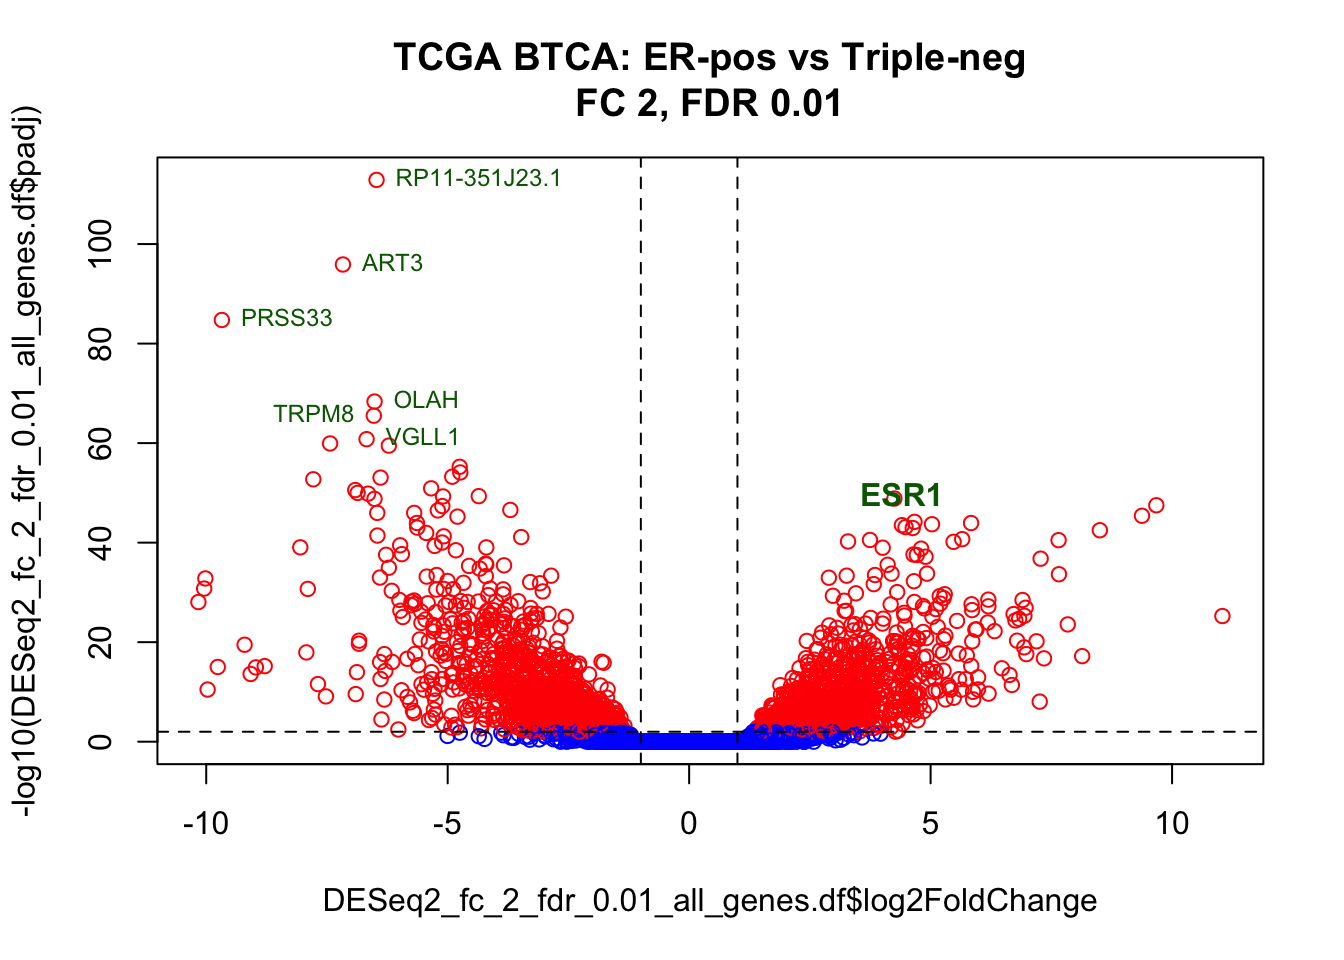
\includegraphics{RNAseq_DEGs_files/figure-latex/unnamed-chunk-32-1.pdf}

\begin{Shaded}
\begin{Highlighting}[]
\CommentTok{# Clean-up}
\KeywordTok{rm}\NormalTok{(genes_color, esr1.df, down_regulated_genes.df)}
\end{Highlighting}
\end{Shaded}

\subsection{Hierarchical clustering using
DEGs}\label{hierarchical-clustering-using-degs}

\textbf{Hierarchical clustering} is also informative to show relations
between samples and top differentially expressed genes

\begin{Shaded}
\begin{Highlighting}[]
\CommentTok{# Libraries for drawing heatmap}
\CommentTok{#install.packages("RColorBrewer")}
\CommentTok{#install.packages("pheatmap")}
\CommentTok{#library(RColorBrewer)}
\CommentTok{#library(pheatmap)}

\CommentTok{# Matrix for clustering and heatmap}
\NormalTok{vst_counts <-}\StringTok{ }\KeywordTok{assay}\NormalTok{(vst_dds)}
\NormalTok{DEGs <-}\StringTok{ }\KeywordTok{rownames}\NormalTok{(vst_counts) }\OperatorTok\StringTok{ }\NormalTok{DESeq2_fc_2_fdr_}\FloatTok{0.}\NormalTok{01_DEGs.df}\OperatorTok{$}\NormalTok{gene_id}
\NormalTok{vst_counts <-}\StringTok{ }\NormalTok{vst_counts[DEGs,]}

\CommentTok{# Scale and center by rows}
\NormalTok{vst_counts <-}\StringTok{ }\KeywordTok{t}\NormalTok{(}\KeywordTok{scale}\NormalTok{(}\KeywordTok{t}\NormalTok{(vst_counts)))}

\CommentTok{# Change genes IDs to genes Names}
\KeywordTok{rownames}\NormalTok{(DESeq2_fc_2_fdr_}\FloatTok{0.}\NormalTok{01_DEGs.df) <-}\StringTok{ }\NormalTok{DESeq2_fc_2_fdr_}\FloatTok{0.}\NormalTok{01_DEGs.df}\OperatorTok{$}\NormalTok{gene_id}
\KeywordTok{rownames}\NormalTok{(vst_counts) <-}\StringTok{ }\NormalTok{DESeq2_fc_2_fdr_}\FloatTok{0.}\NormalTok{01_DEGs.df[}\KeywordTok{rownames}\NormalTok{(vst_counts),}\StringTok{"gene_name"}\NormalTok{]}

\CommentTok{# Data frame with ER- and OCT- status}
\NormalTok{cases.df <-}\StringTok{ }\KeywordTok{as.data.frame}\NormalTok{(}\KeywordTok{colData}\NormalTok{(vst_dds))}
\NormalTok{cases.df <-}\StringTok{ }\NormalTok{cases.df }\OperatorTok\StringTok{ }\KeywordTok{select}\NormalTok{(oct, er)}

\CommentTok{# Make palette of 99 colours for heatmap}
\NormalTok{gbr_}\DecValTok{99}\NormalTok{ <-}\StringTok{ }\KeywordTok{colorRampPalette}\NormalTok{(}\KeywordTok{c}\NormalTok{(}\StringTok{"green"}\NormalTok{, }\StringTok{"black"}\NormalTok{, }\StringTok{"red"}\NormalTok{))(}\DataTypeTok{n =} \DecValTok{99}\NormalTok{)}

\CommentTok{# Make breaks between colours by 100 quantiles }
\NormalTok{breaks_}\DecValTok{100}\NormalTok{ <-}\StringTok{ }\KeywordTok{quantile}\NormalTok{(vst_counts, }\DataTypeTok{probs=}\KeywordTok{seq}\NormalTok{(}\DecValTok{0}\NormalTok{,}\DecValTok{1}\NormalTok{,}\DataTypeTok{length.out=}\DecValTok{100}\NormalTok{))}

\CommentTok{# Plot the heatmap and dendrograms}
\CommentTok{# Row and column names couls be shown if there was a smaller number of genes and samples}
\CommentTok{# Options "fontsize_row" and "fontsize_col" could be used for row/column labels adjustment }
\KeywordTok{pheatmap}\NormalTok{(}
  \DataTypeTok{mat =}\NormalTok{ vst_counts, }\CommentTok{# matrix with data}
  \DataTypeTok{color =}\NormalTok{ gbr_}\DecValTok{99}\NormalTok{, }\CommentTok{# user-defined palette}
  \DataTypeTok{breaks =}\NormalTok{ breaks_}\DecValTok{100}\NormalTok{, }\CommentTok{# user-defined breaks between colours}
  \DataTypeTok{annotation_col =}\NormalTok{ cases.df, }\CommentTok{# ER- and OCT- status}
  \DataTypeTok{scale =} \StringTok{"none"}\NormalTok{, }\CommentTok{# has been scaled manually}
  \DataTypeTok{border_color =} \OtherTok{NA}\NormalTok{, }\CommentTok{# dont draw borders in heatmap}
  \DataTypeTok{show_rownames =} \OtherTok{FALSE}\NormalTok{, }\CommentTok{# too many genes to show names}
  \DataTypeTok{show_colnames =} \OtherTok{FALSE}\NormalTok{, }\CommentTok{# too many samples to show names}
  \DataTypeTok{main =} \StringTok{"HC with top DEGs"}\NormalTok{)}

\CommentTok{# Clean-up}
\KeywordTok{rm}\NormalTok{(vst_counts, gbr_}\DecValTok{99}\NormalTok{, breaks_}\DecValTok{100}\NormalTok{, cases.df, DEGs)}
\end{Highlighting}
\end{Shaded}

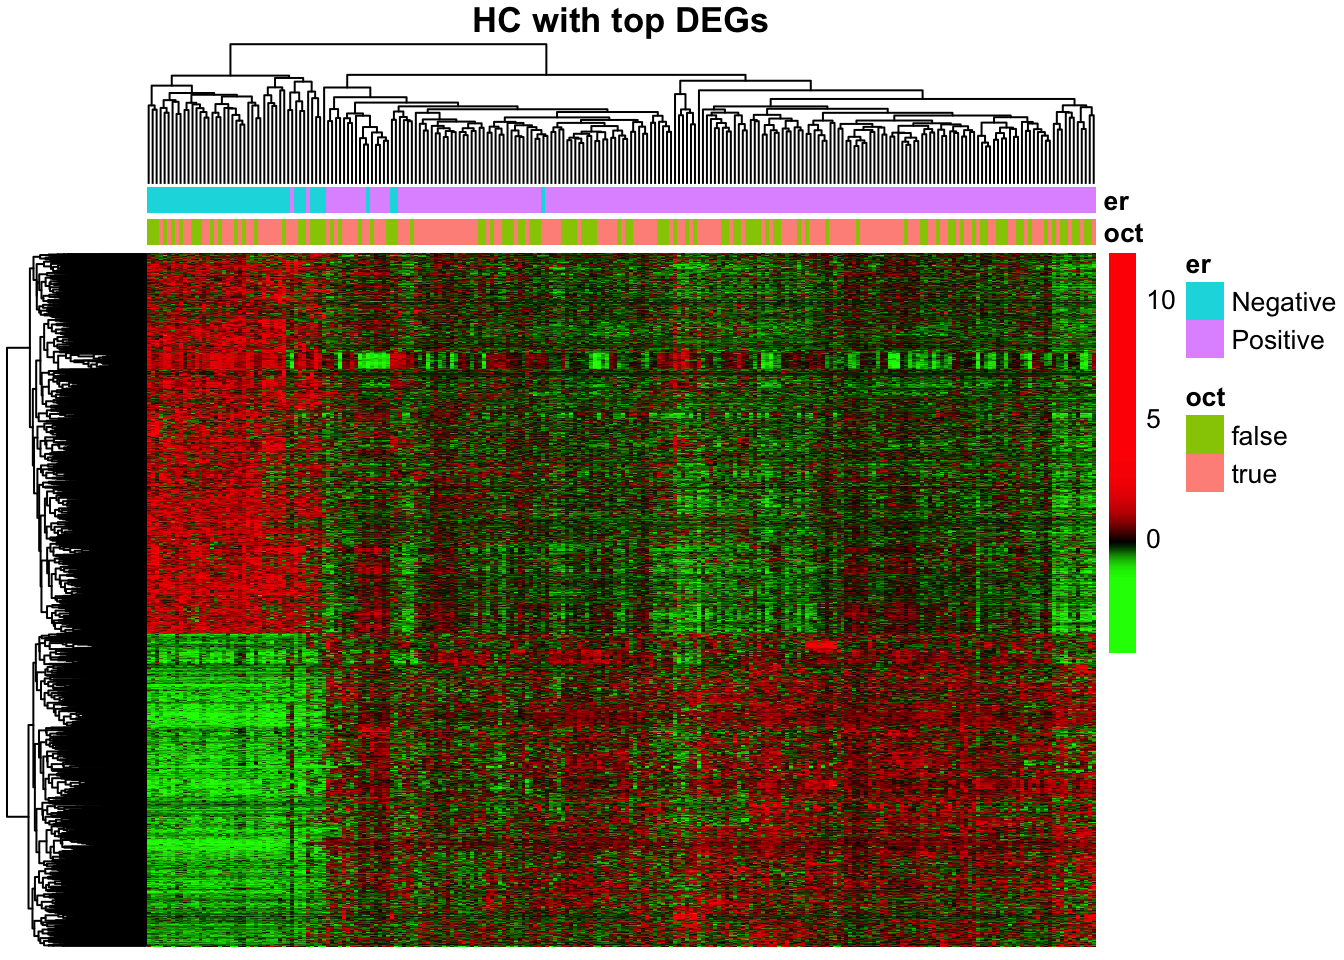
\includegraphics[width=1\linewidth]{/Users/alexey/OneDrive/Documents/Teaching/Lecturing/rna-seq-ebi-2020-tutorial/analysis/figures/f03_hc_2k}

\section{Save results}\label{save-results}

You can use \textbf{write.table} function to save DEGs (and results for
all genes) to a text file:

\begin{Shaded}
\begin{Highlighting}[]
\CommentTok{# Save DEGs}
\KeywordTok{write.table}\NormalTok{(DESeq2_fc_2_fdr_}\FloatTok{0.}\NormalTok{01_DEGs.df, }
            \DataTypeTok{file=}\KeywordTok{file.path}\NormalTok{(base_folder,}\StringTok{"analysis"}\NormalTok{,}\StringTok{"results"}\NormalTok{,}\StringTok{"DESeq2_fc_2_fdr_0_01_DEGs.txt"}\NormalTok{),}
            \DataTypeTok{quote=}\NormalTok{F, }\DataTypeTok{sep=}\StringTok{"}\CharTok{\textbackslash{}t}\StringTok{"}\NormalTok{, }\DataTypeTok{row.names =}\NormalTok{ F)}

\CommentTok{# Save all genes}
\KeywordTok{write.table}\NormalTok{(DESeq2_fc_2_fdr_}\FloatTok{0.}\NormalTok{01_all_genes.df, }
            \DataTypeTok{file=}\KeywordTok{file.path}\NormalTok{(base_folder,}\StringTok{"analysis"}\NormalTok{,}\StringTok{"results"}\NormalTok{,}\StringTok{"DESeq2_fc_2_fdr_0_01_all_genes.txt"}\NormalTok{),}
            \DataTypeTok{quote=}\NormalTok{F, }\DataTypeTok{sep=}\StringTok{"}\CharTok{\textbackslash{}t}\StringTok{"}\NormalTok{, }\DataTypeTok{row.names =}\NormalTok{ F)}
\end{Highlighting}
\end{Shaded}

\chapter{edgeR analysis}\label{edger-analysis-1}

First, we load edgeR library:

\begin{Shaded}
\begin{Highlighting}[]
\CommentTok{#install.packages("BiocManager")}
\CommentTok{#BiocManager::install("edgeR")}
\KeywordTok{suppressWarnings}\NormalTok{(}\KeywordTok{suppressMessages}\NormalTok{(}\KeywordTok{library}\NormalTok{(edgeR)))}
\end{Highlighting}
\end{Shaded}

\section{Read HTSeq counts to
DGEList}\label{read-htseq-counts-to-dgelist}

Prior the analysis \textbf{edgeR} needs to collect all necessary
information. \textbf{edgeR} collects the counts, samples and genes data
in a single list called \textbf{DGEList}. To facilitate the data input
\textbf{edgeR} provides a function called \textbf{readDGE} that makes a
single matrix from multiple files, allows adding sample information etc.

The function can read tabulated text files of arbitrary format, as long
as one of the file's columns contains genes names and another column
contains the counts. Format of an HTSeq counts file can be explored
using \textbf{Bash} functions \textbf{head} and \textbf{tail}:

\begin{verbatim}
## ENSG00000000003.13   2569
## ENSG00000000005.5    1
## ENSG00000000419.11   3180
## ENSG00000000457.12   3332
## ENSG00000000460.15   1621
## ENSG00000000938.11   530
## ENSG00000000971.14   7282
## ENSG00000001036.12   3312
## ENSG00000001084.9    2642
## ENSG00000001167.13   3322
## ...
## ENSGR0000275287.3    0
## ENSGR0000276543.3    0
## ENSGR0000277120.3    0
## ENSGR0000280767.1    0
## ENSGR0000281849.1    0
## __no_feature 3069305
## __ambiguous  3368739
## __too_low_aQual  0
## __not_aligned    0
## __alignment_not_unique   23748640
\end{verbatim}

It can be seen that an \textbf{HTSeq counts file} fits \textbf{readDGE}
requirements, except for some summary lines at the end of the file.
Luckily, \textbf{readDGE} can take care about these summary lines with
\textbf{comment.char} option. Finally, \textbf{header = FALSE} should be
used to specify that the 1st row contains data, not the header:

\begin{Shaded}
\begin{Highlighting}[]
\CommentTok{# Counts folder}
\NormalTok{counts_folder=}\KeywordTok{file.path}\NormalTok{(base_folder,}\StringTok{"data"}\NormalTok{,}\StringTok{"HTSeq_counts"}\NormalTok{)}

\CommentTok{# Read HTSeq counts to DGE object}
\CommentTok{# ("dgl" stands for "DGEList")}
\NormalTok{dgl <-}\StringTok{ }\KeywordTok{readDGE}\NormalTok{(}\DataTypeTok{files=}\NormalTok{samples.df}\OperatorTok{$}\NormalTok{file, }\CommentTok{# files names}
        \DataTypeTok{path=}\NormalTok{counts_folder, }\CommentTok{# folder with count files}
        \DataTypeTok{columns=}\KeywordTok{c}\NormalTok{(}\DecValTok{1}\NormalTok{,}\DecValTok{2}\NormalTok{), }\CommentTok{# columns with gene name (1) and count (2)}
        \DataTypeTok{labels=}\NormalTok{samples.df}\OperatorTok{$}\NormalTok{patient, }\CommentTok{# samples names corresponding to the files}
        \DataTypeTok{comment.char=}\StringTok{"_"}\NormalTok{, }\CommentTok{# lines starting with this character are excluded}
        \DataTypeTok{header =} \OtherTok{FALSE}\NormalTok{) }\CommentTok{# the 1st row contains data, not header}

\CommentTok{# Clean-up}
\KeywordTok{rm}\NormalTok{(counts_folder)}
\end{Highlighting}
\end{Shaded}

See \textbf{readDGE} help for details of other options used in the above
command.

\section{Explore and update the DEGList
object}\label{explore-and-update-the-deglist-object}

The code chunk below

\begin{itemize}
\tightlist
\item
  checks content of the counts' matrix read to the DEGList object\\
\item
  checks samples information and adds OCT-status as an example of
  potential experimental confounder\\
\item
  adds genes information to the DEGList object
\end{itemize}

See \textbf{DEGList} help for details.

\begin{Shaded}
\begin{Highlighting}[]
\CommentTok{# Check content of created DEGList}
\KeywordTok{names}\NormalTok{(dgl)}
\end{Highlighting}
\end{Shaded}

\begin{verbatim}
## [1] "samples" "counts"
\end{verbatim}

\begin{Shaded}
\begin{Highlighting}[]
\CommentTok{# The counts matrix is identical to the counts in DESeq2DataSet}
\KeywordTok{dim}\NormalTok{(dgl}\OperatorTok{$}\NormalTok{counts)}
\end{Highlighting}
\end{Shaded}

\begin{verbatim}
## [1] 60483   238
\end{verbatim}

\begin{Shaded}
\begin{Highlighting}[]
\NormalTok{dgl}\OperatorTok{$}\NormalTok{counts[}\DecValTok{1}\OperatorTok{:}\DecValTok{5}\NormalTok{,}\DecValTok{1}\OperatorTok{:}\DecValTok{5}\NormalTok{]}
\end{Highlighting}
\end{Shaded}

\begin{verbatim}
##                     Samples
## Tags                 TCGA-A7-A0DA TCGA-D8-A1XU TCGA-D8-A143 TCGA-A7-A4SB TCGA-D8-A1XR
##   ENSG00000000003.13         2724         5645         6180         2558         3884
##   ENSG00000000005.5             7            6            1           32          109
##   ENSG00000000419.11         1962         4926         2624         1068         3337
##   ENSG00000000457.12         1973         2271         1860         1362         4953
##   ENSG00000000460.15          867          675         2359          494         2284
\end{verbatim}

\begin{Shaded}
\begin{Highlighting}[]
\CommentTok{# Add information about the exparimental groups for DEG detection (ER status)  }
\KeywordTok{head}\NormalTok{(dgl}\OperatorTok{$}\NormalTok{samples)}
\end{Highlighting}
\end{Shaded}

\begin{verbatim}
##                                                             files group lib.size norm.factors
## TCGA-A7-A0DA a33029dd-b5fa-4be0-9cbf-971d289146dd.htseq.counts.gz     1 66687895            1
## TCGA-D8-A1XU 8d54214a-1d9b-4fea-9c42-5bbb3cd11da9.htseq.counts.gz     1 93109355            1
## TCGA-D8-A143 4b19c0e2-2a61-4f0a-9257-4a528e6b320e.htseq.counts.gz     1 55477594            1
## TCGA-A7-A4SB cc233ff9-d5fb-4e9b-9007-f58d008df995.htseq.counts.gz     1 38870554            1
## TCGA-D8-A1XR bdd8c340-250b-474a-8802-7653b7884ced.htseq.counts.gz     1 82295968            1
## TCGA-BH-A18L 5bc7e90d-0fa4-4bde-bee8-4f9b92de03a2.htseq.counts.gz     1 71552576            1
\end{verbatim}

\begin{Shaded}
\begin{Highlighting}[]
\CommentTok{# Add ER and OCT status to the samples information}
\NormalTok{dgl}\OperatorTok{$}\NormalTok{samples}\OperatorTok{$}\NormalTok{er <-}\StringTok{ }\NormalTok{samples.df}\OperatorTok{$}\NormalTok{er}
\NormalTok{dgl}\OperatorTok{$}\NormalTok{samples}\OperatorTok{$}\NormalTok{oct <-}\StringTok{ }\NormalTok{samples.df}\OperatorTok{$}\NormalTok{oct}
\KeywordTok{head}\NormalTok{(dgl}\OperatorTok{$}\NormalTok{samples)}
\end{Highlighting}
\end{Shaded}

\begin{verbatim}
##                                                             files group lib.size norm.factors       er   oct
## TCGA-A7-A0DA a33029dd-b5fa-4be0-9cbf-971d289146dd.htseq.counts.gz     1 66687895            1 Negative false
## TCGA-D8-A1XU 8d54214a-1d9b-4fea-9c42-5bbb3cd11da9.htseq.counts.gz     1 93109355            1 Positive false
## TCGA-D8-A143 4b19c0e2-2a61-4f0a-9257-4a528e6b320e.htseq.counts.gz     1 55477594            1 Negative false
## TCGA-A7-A4SB cc233ff9-d5fb-4e9b-9007-f58d008df995.htseq.counts.gz     1 38870554            1 Positive false
## TCGA-D8-A1XR bdd8c340-250b-474a-8802-7653b7884ced.htseq.counts.gz     1 82295968            1 Positive false
## TCGA-BH-A18L 5bc7e90d-0fa4-4bde-bee8-4f9b92de03a2.htseq.counts.gz     1 71552576            1 Positive  true
\end{verbatim}

\begin{Shaded}
\begin{Highlighting}[]
\CommentTok{# Add genes information}
\NormalTok{genes.df <-}\StringTok{ }\NormalTok{genes.df[}\KeywordTok{rownames}\NormalTok{(dgl}\OperatorTok{$}\NormalTok{counts),] }\CommentTok{# Reorder genes to match the genes order in the counts matrix}
\NormalTok{dgl}\OperatorTok{$}\NormalTok{genes <-}\StringTok{ }\NormalTok{genes.df}
\KeywordTok{names}\NormalTok{(dgl)}
\end{Highlighting}
\end{Shaded}

\begin{verbatim}
## [1] "samples" "counts"  "genes"
\end{verbatim}

\section{Gene filtering}\label{gene-filtering}

In \textbf{DESeq2} analysis we manually removed genes, for which less
than 10 samples had count above 10. This reduced the nimber of genes
from \textasciitilde{}60k to \textasciitilde{}28k.

\textbf{edgrR} has a dedicated build-in function \textbf{filterByExpr}
to remove low-expressed genes. This function also keeps the genes with a
count above 10 in a certain number of samples, depending in the groups
size. Applying this function to our TCGA-BRCA dataset preserves
\textasciitilde{}24k of genes, which is reasonably close to the manual
filtering applyed in DESeq2 analysis.

\begin{Shaded}
\begin{Highlighting}[]
\CommentTok{# Select genes with sufficien expression for comparison in ER groups}
\NormalTok{keep.exprs <-}\StringTok{ }\KeywordTok{filterByExpr}\NormalTok{(dgl, }\DataTypeTok{group=}\NormalTok{dgl}\OperatorTok{$}\NormalTok{samples}\OperatorTok{$}\NormalTok{er)}
\KeywordTok{sum}\NormalTok{(keep.exprs)}
\end{Highlighting}
\end{Shaded}

\begin{verbatim}
## [1] 24361
\end{verbatim}

\begin{Shaded}
\begin{Highlighting}[]
\CommentTok{# Remove low-expressed genes }
\NormalTok{dgl <-}\StringTok{ }\NormalTok{dgl[keep.exprs,, keep.lib.sizes=}\OtherTok{FALSE}\NormalTok{]}
\KeywordTok{dim}\NormalTok{(dgl)}
\end{Highlighting}
\end{Shaded}

\begin{verbatim}
## [1] 24361   238
\end{verbatim}

\begin{Shaded}
\begin{Highlighting}[]
\CommentTok{# Clean-up}
\KeywordTok{rm}\NormalTok{(keep.exprs)}
\end{Highlighting}
\end{Shaded}

\section{Normalizing by TMM}\label{normalizing-by-tmm}

\textbf{edgeR}'s preferred method of normalization is \textbf{Trimmed
Means of M-values} (TMM)

\begin{Shaded}
\begin{Highlighting}[]
\CommentTok{# Aply normalization}
\NormalTok{dgl <-}\StringTok{ }\KeywordTok{calcNormFactors}\NormalTok{(dgl, }\DataTypeTok{method =} \StringTok{"TMM"}\NormalTok{)}

\CommentTok{# Look at the calculated TMM notmalization factors}
\KeywordTok{plot}\NormalTok{(dgl}\OperatorTok{$}\NormalTok{samples}\OperatorTok{$}\NormalTok{norm.factors, }\DataTypeTok{main=}\StringTok{"Normalization factors"}\NormalTok{)}
\end{Highlighting}
\end{Shaded}

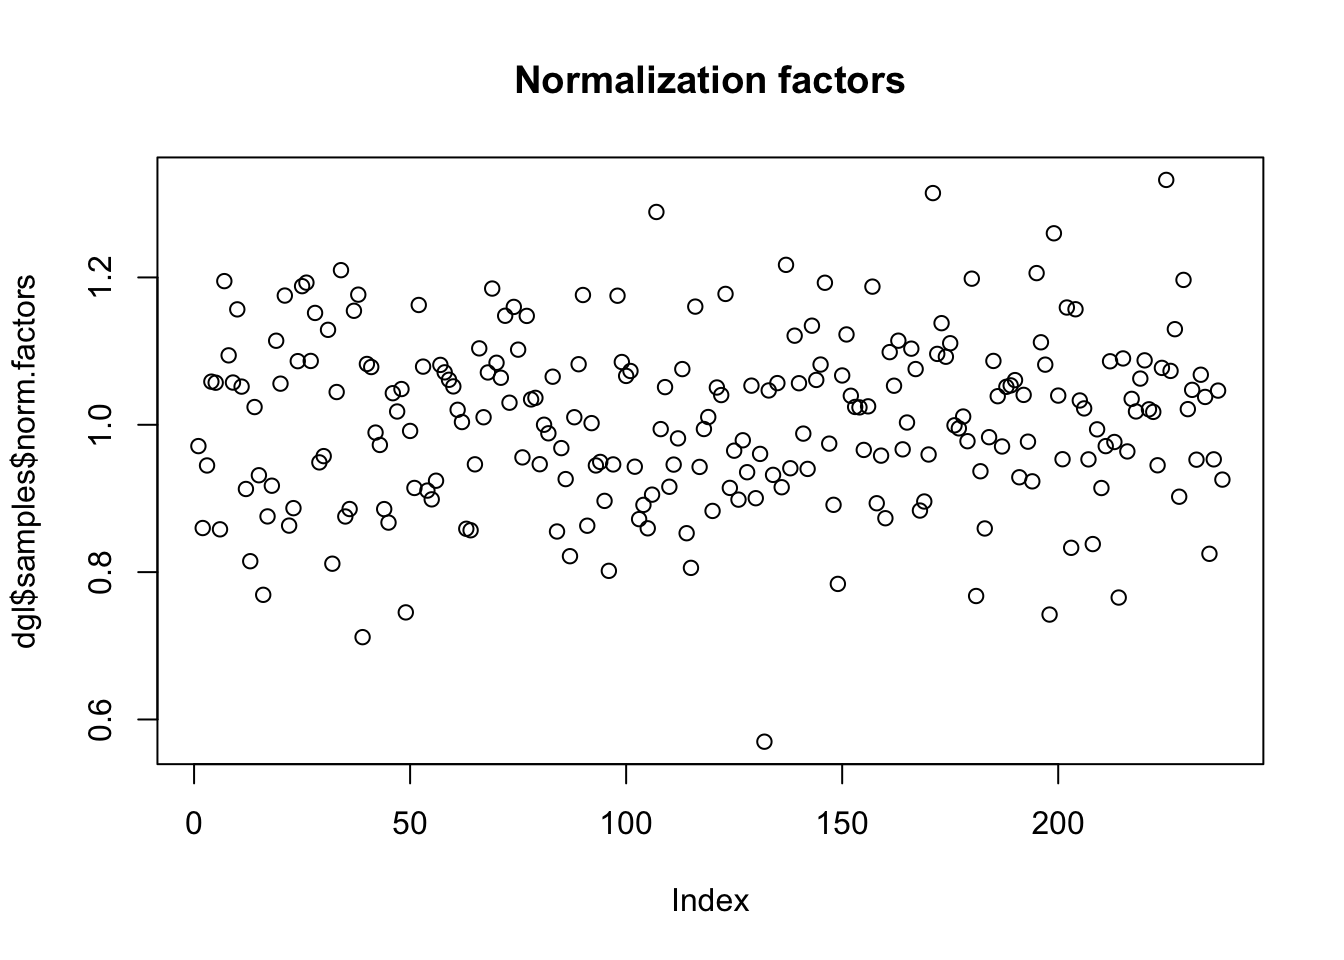
\includegraphics{RNAseq_DEGs_files/figure-latex/unnamed-chunk-42-1.pdf}

\section{Exploring source data}\label{exploring-source-data-1}

Like in \textbf{DESeq2} analysis, the source data is explored in a
normalized form. For this, \textbf{edgeR} allows to calculate
log-transformed counts per million:

\begin{Shaded}
\begin{Highlighting}[]
\NormalTok{lcpm <-}\StringTok{ }\KeywordTok{cpm}\NormalTok{(dgl, }\DataTypeTok{log=}\OtherTok{TRUE}\NormalTok{)}
\end{Highlighting}
\end{Shaded}

\subsection{Boxplot}\label{boxplot}

The boxplot shows that counts range and central positions are similar in
different samples after the normalization:

\begin{Shaded}
\begin{Highlighting}[]
\KeywordTok{boxplot}\NormalTok{(lcpm, }\DataTypeTok{xaxt=}\StringTok{"n"}\NormalTok{, }\DataTypeTok{main=}\StringTok{"Normalized log-transformed data"}\NormalTok{,}
        \DataTypeTok{xlab=}\StringTok{"Samples"}\NormalTok{,}\DataTypeTok{ylab=}\StringTok{"Log(normalized counts)"}\NormalTok{)}
\end{Highlighting}
\end{Shaded}

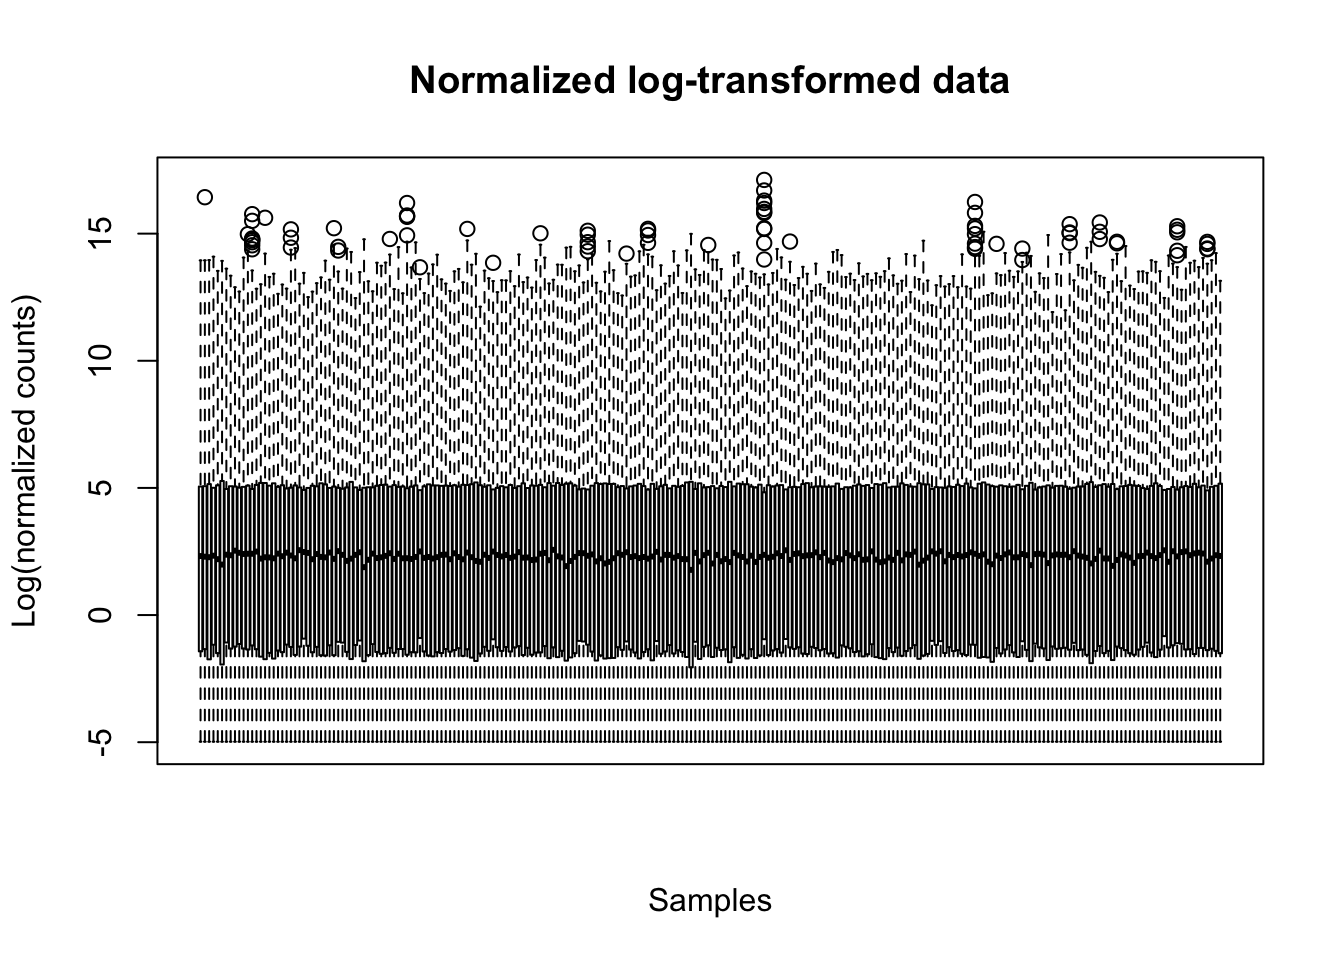
\includegraphics{RNAseq_DEGs_files/figure-latex/unnamed-chunk-44-1.pdf}

\subsection{MDS plot}\label{mds-plot}

Multi Dimentional Scaling (MDS) is similar to PCA: it places similar
samples close to each other in a 2-dimention plot. \textbf{edgeR}
provides a function for making a MDS plot. The plot shows a clear
separation of ER-positive and Triple-negative breast cancers by the
genes expression.

\begin{Shaded}
\begin{Highlighting}[]
\CommentTok{# Colour code ER status}
\NormalTok{col_er <-}\StringTok{ }\KeywordTok{as.factor}\NormalTok{(dgl}\OperatorTok{$}\NormalTok{samples}\OperatorTok{$}\NormalTok{er)}
\KeywordTok{levels}\NormalTok{(col_er) <-}\StringTok{ }\KeywordTok{c}\NormalTok{(}\StringTok{"blue"}\NormalTok{,}\StringTok{"red"}\NormalTok{)}
\NormalTok{col_er <-}\StringTok{ }\KeywordTok{as.character}\NormalTok{(col_er)}

\CommentTok{# Make MDS plot}
\KeywordTok{plotMDS}\NormalTok{(lcpm, }\DataTypeTok{labels =} \OtherTok{NULL}\NormalTok{, }\DataTypeTok{pch =} \DecValTok{1}\NormalTok{, }\DataTypeTok{col=}\NormalTok{col_er,}
        \DataTypeTok{main=}\StringTok{"MDS plot"}\NormalTok{)}

\KeywordTok{legend}\NormalTok{(}\StringTok{"topright"}\NormalTok{, }\CommentTok{# the location of the legend on the plot}
       \DataTypeTok{legend =} \KeywordTok{c}\NormalTok{(}\StringTok{"ER-neg"}\NormalTok{, }\StringTok{"ER-pos"}\NormalTok{), }\CommentTok{# labels}
       \DataTypeTok{col =} \KeywordTok{c}\NormalTok{(}\StringTok{"blue"}\NormalTok{,}\StringTok{"red"}\NormalTok{),}
       \DataTypeTok{pch =} \DecValTok{1}\NormalTok{) }\CommentTok{# colours}
\end{Highlighting}
\end{Shaded}

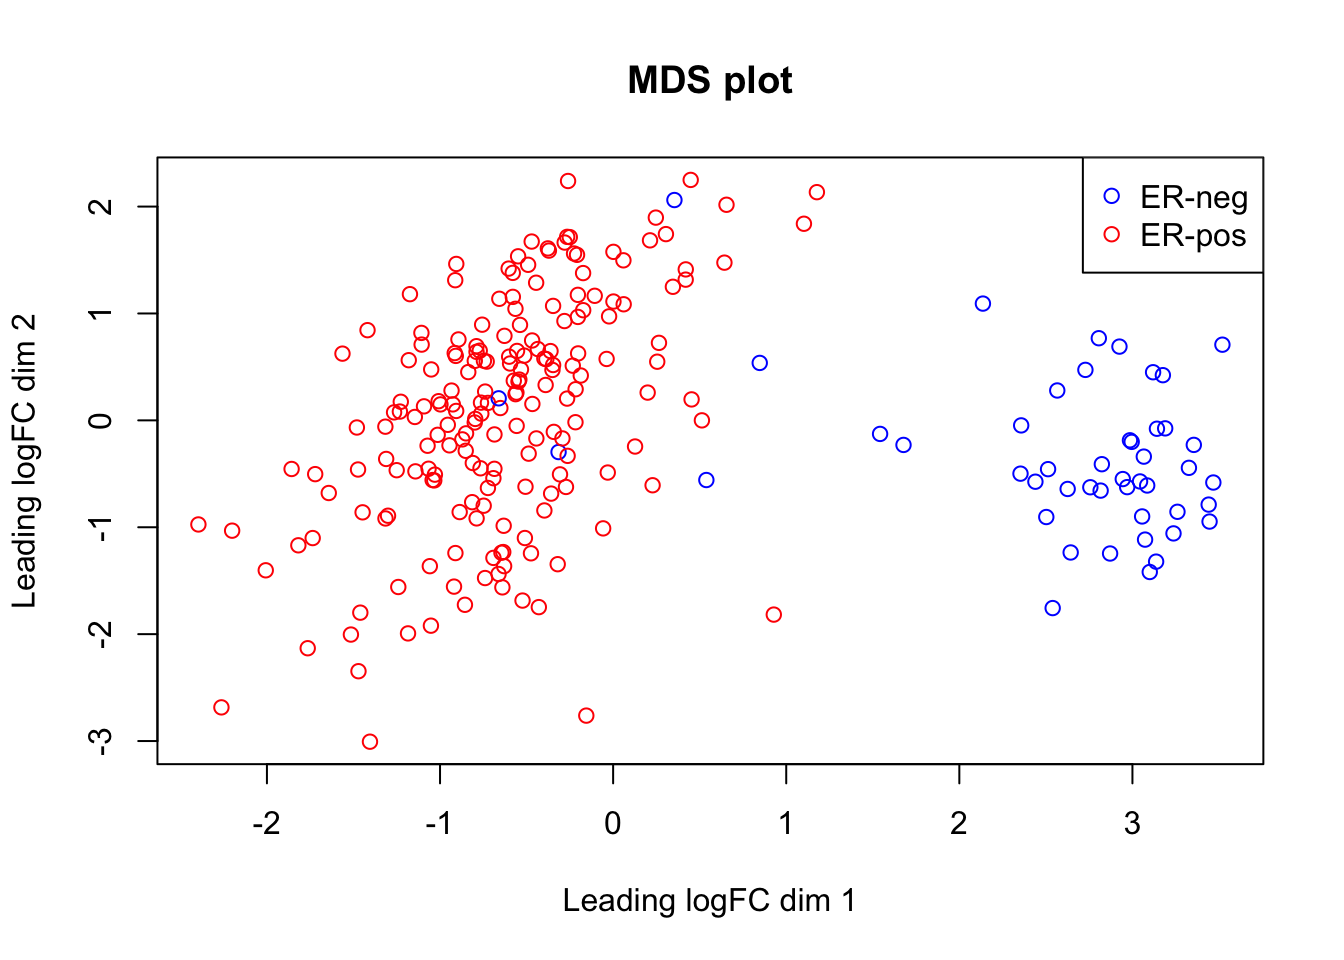
\includegraphics{RNAseq_DEGs_files/figure-latex/unnamed-chunk-45-1.pdf}

\begin{Shaded}
\begin{Highlighting}[]
\CommentTok{# Clean-up}
\KeywordTok{rm}\NormalTok{(lcpm, col_er)}
\end{Highlighting}
\end{Shaded}

\section{Calculate DEGs}\label{calculate-degs}

\subsection{Specify design}\label{specify-design}

Like in \textbf{DESeq2} the design in \textbf{edgeR} is defined by a
text string that follows the format of a \textbf{glm} formula in R:
\textbf{\textasciitilde{} oct + er}. It is used to specify the variable
of interest for differential expression (``er''" in our case) and the
confounding variables, if any (``oct'' in our case). By convention, the
variable of interest should be placed is at the end of the design
formula.

\begin{Shaded}
\begin{Highlighting}[]
\NormalTok{design <-}\StringTok{ }\KeywordTok{model.matrix}\NormalTok{(}\OperatorTok{~}\StringTok{ }\NormalTok{oct }\OperatorTok{+}\StringTok{ }\NormalTok{er, }\DataTypeTok{data =}\NormalTok{ dgl}\OperatorTok{$}\NormalTok{samples)}
\end{Highlighting}
\end{Shaded}

\subsection{Estimate dispersions}\label{estimate-dispersions}

Like in \textbf{DESeq2}, the variance estimation and adjustment is a
core element of building the \textbf{edgeR} statistical model:

\begin{Shaded}
\begin{Highlighting}[]
\NormalTok{dgl <-}\StringTok{ }\KeywordTok{estimateDisp}\NormalTok{(dgl, design)}
\KeywordTok{plotBCV}\NormalTok{(dgl, }\DataTypeTok{main=}\StringTok{"Dispersion estimates and adjustments"}\NormalTok{)}
\end{Highlighting}
\end{Shaded}

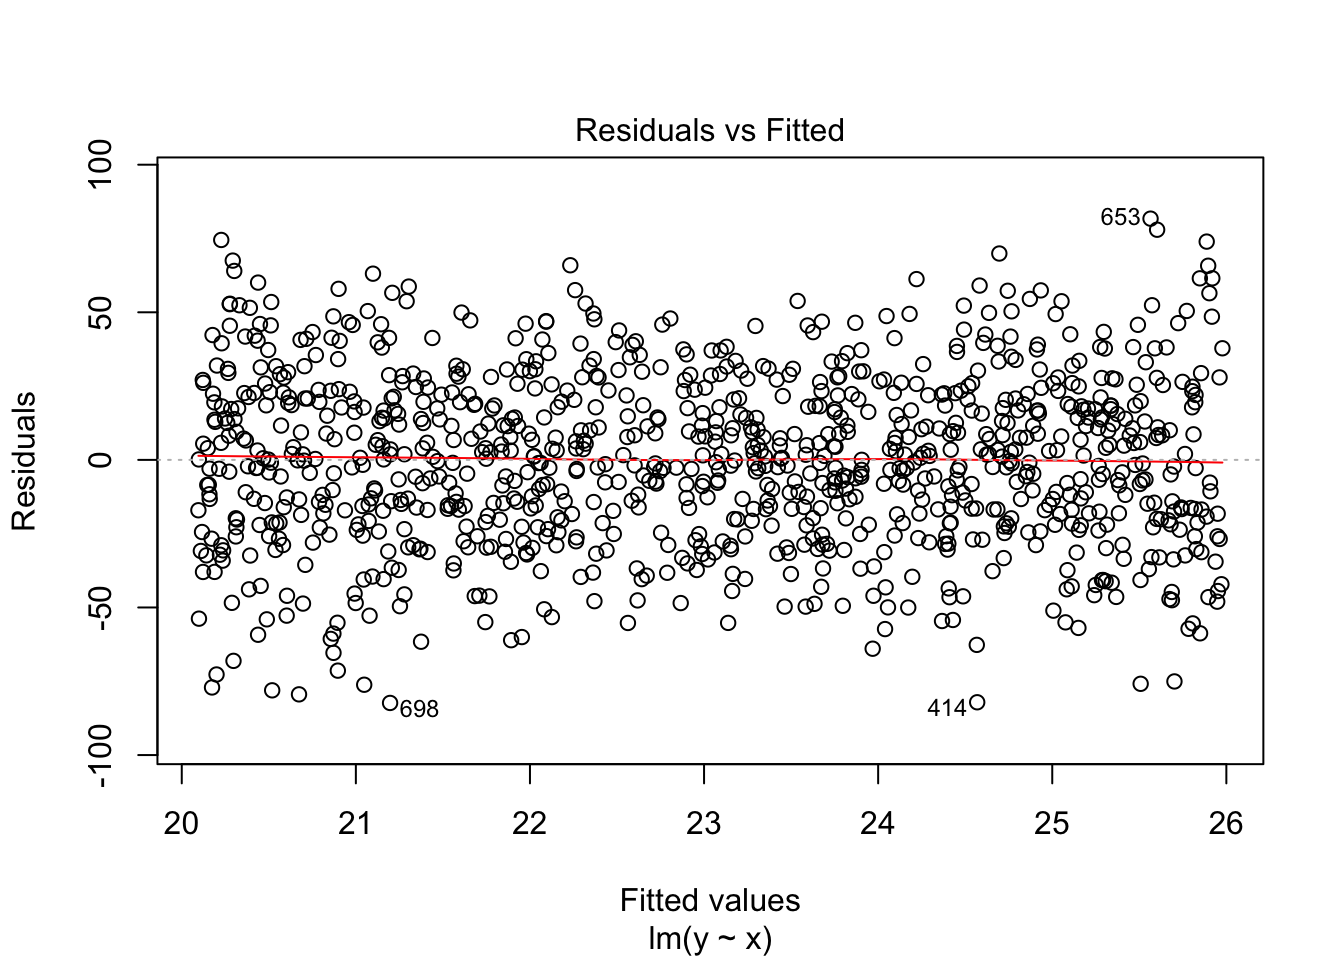
\includegraphics{RNAseq_DEGs_files/figure-latex/unnamed-chunk-47-1.pdf}

\subsection{Fit the model}\label{fit-the-model}

\begin{Shaded}
\begin{Highlighting}[]
\NormalTok{fit <-}\StringTok{ }\KeywordTok{glmQLFit}\NormalTok{(dgl, design)}
\end{Highlighting}
\end{Shaded}

\section{Extract results}\label{extract-results}

The gene-wise statistical significance is extracted from the model,
which has been fitted in the previous code chunk.

\subsection{Default settings}\label{default-settings}

By default edgeR calculates tests against the null hypothesis of no
change (i.e. \textbf{alt hypothesis of any change}). The key results are
written in the \textbf{table} slot of the specialised \textbf{TopTags}
result object.

Note that in \textbf{glmQLFTest} function call the
\textbf{coef=ncol(design)} points to the last column in the design
table. You may remember that,by convention, the variable of interest was
placed at the end of the design formula.

The \textbf{topTags} function actually prepared the table with results.
By default, though, it will only show the top 10 genes\ldots{} To
extract results for all the genes \textbf{n = nrow(x)} option is used.

\begin{Shaded}
\begin{Highlighting}[]
\CommentTok{# Calculate the test statistics}
\NormalTok{edgeR_any_change <-}\StringTok{ }\KeywordTok{glmQLFTest}\NormalTok{(fit, }\DataTypeTok{coef =} \KeywordTok{ncol}\NormalTok{(design))}

\CommentTok{# Extract statistics for all genes}
\NormalTok{edgeR_any_change_all_genes <-}\StringTok{ }\KeywordTok{topTags}\NormalTok{(edgeR_any_change, }\DataTypeTok{n =} \KeywordTok{nrow}\NormalTok{(dgl), }\DataTypeTok{sort.by =} \StringTok{"none"}\NormalTok{)}
\KeywordTok{names}\NormalTok{(edgeR_any_change_all_genes)}
\end{Highlighting}
\end{Shaded}

\begin{verbatim}
## [1] "table"         "adjust.method" "comparison"    "test"
\end{verbatim}

\begin{Shaded}
\begin{Highlighting}[]
\CommentTok{# Explore table with results}
\KeywordTok{dim}\NormalTok{(edgeR_any_change_all_genes}\OperatorTok{$}\NormalTok{table)}
\end{Highlighting}
\end{Shaded}

\begin{verbatim}
## [1] 24361     7
\end{verbatim}

\begin{Shaded}
\begin{Highlighting}[]
\KeywordTok{head}\NormalTok{(edgeR_any_change_all_genes}\OperatorTok{$}\NormalTok{table)}
\end{Highlighting}
\end{Shaded}

\begin{verbatim}
##                               gene_id gene_name      logFC      logCPM        F       PValue          FDR
## ENSG00000000003.13 ENSG00000000003.13    TSPAN6 -0.6784647  5.73670542 23.82900 1.925960e-06 6.531856e-06
## ENSG00000000005.5   ENSG00000000005.5      TNMD  1.8310633 -0.08050533 18.95597 1.984714e-05 5.666193e-05
## ENSG00000000419.11 ENSG00000000419.11      DPM1 -0.3582450  5.25058484 18.56443 2.400762e-05 6.752680e-05
## ENSG00000000457.12 ENSG00000000457.12     SCYL3  0.3891598  5.09050998 18.72840 2.216723e-05 6.275607e-05
## ENSG00000000460.15 ENSG00000000460.15  C1orf112 -0.8041035  3.83330744 54.05200 3.092747e-12 2.434327e-11
## ENSG00000000938.11 ENSG00000000938.11       FGR -0.1688074  3.34761965  1.27565 2.598416e-01 3.256509e-01
\end{verbatim}

Like in \textbf{DESeq2} analysis, the default settings lead to an
inflated number of \textbf{significant} p-values (if compared to the
expected uniform distribution of p-values under the null):

\begin{Shaded}
\begin{Highlighting}[]
\CommentTok{# Plot histogram of p-values}
\KeywordTok{hist}\NormalTok{(edgeR_any_change_all_genes}\OperatorTok{$}\NormalTok{table}\OperatorTok{$}\NormalTok{PValue)}
\end{Highlighting}
\end{Shaded}

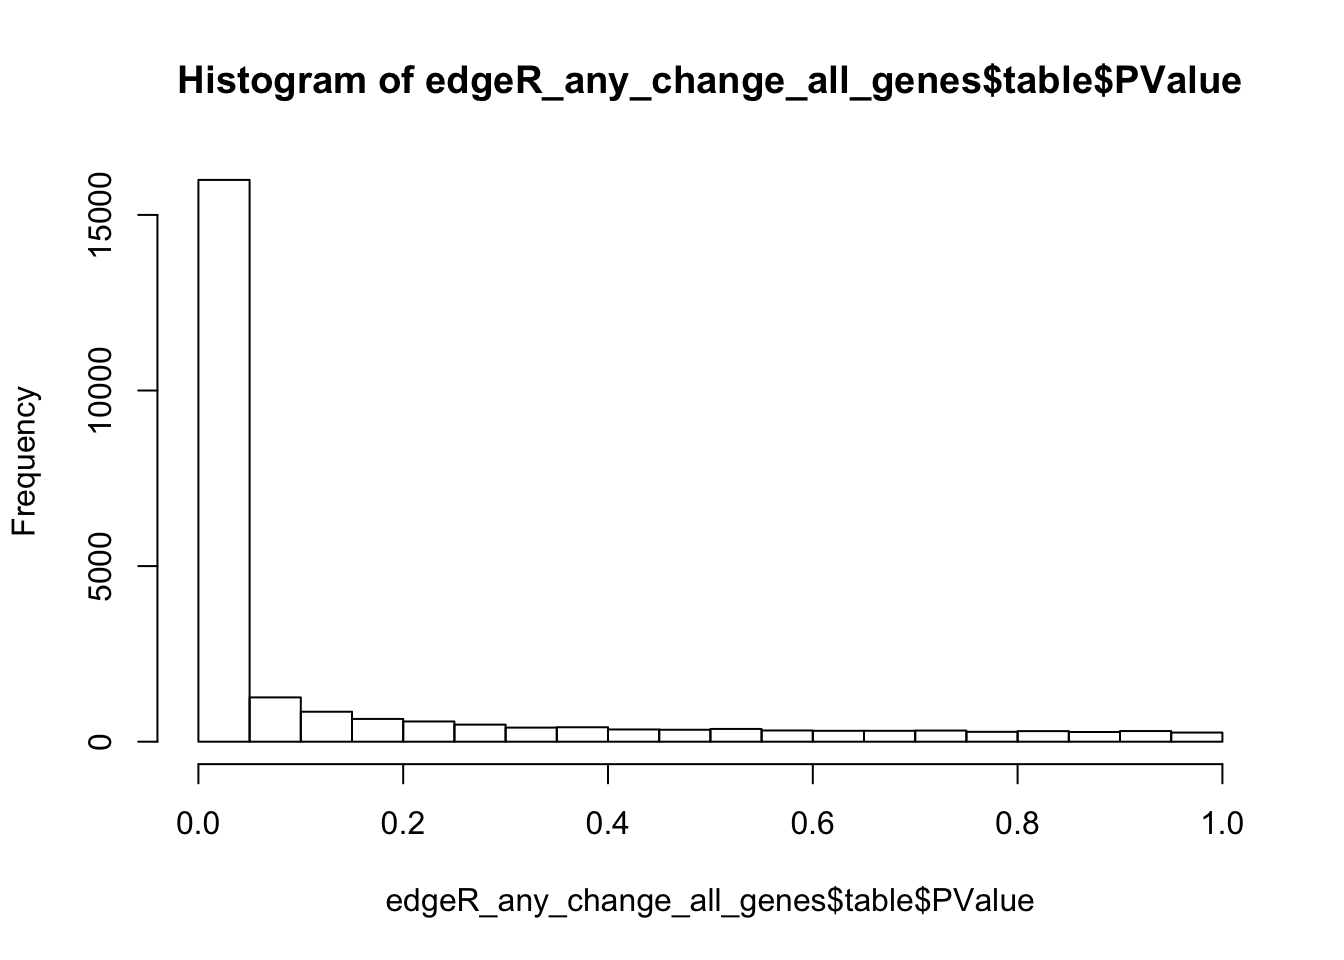
\includegraphics{RNAseq_DEGs_files/figure-latex/unnamed-chunk-50-1.pdf}

By default, the \textbf{topTags} function does not apply a filter by
p-value. However, such option exists. In the chunk below we apply a FDR
0.1 filter, by analogy with the default FDR threshold in
\textbf{DESeq2}. Like in \textbf{DESeq2} analysis such thersholds would
suggest that more than half of the genes are differentially expressed:

\begin{Shaded}
\begin{Highlighting}[]
\CommentTok{# Select genes with FDR 0.1}
\NormalTok{edgeR_any_change_fdr_}\FloatTok{0.1}\NormalTok{ <-}\StringTok{ }\KeywordTok{topTags}\NormalTok{(edgeR_any_change, }\DataTypeTok{n =} \KeywordTok{nrow}\NormalTok{(dgl), }\DataTypeTok{p.value =} \FloatTok{0.1}\NormalTok{)}
\KeywordTok{dim}\NormalTok{(edgeR_any_change_fdr_}\FloatTok{0.1}\OperatorTok{$}\NormalTok{table)}
\end{Highlighting}
\end{Shaded}

\begin{verbatim}
## [1] 16575     7
\end{verbatim}

MA plot in \textbf{edgeR} is plotted by \textbf{plotSmear} function:

\begin{Shaded}
\begin{Highlighting}[]
\KeywordTok{plotSmear}\NormalTok{(edgeR_any_change, }\DataTypeTok{de.tags =}\NormalTok{ edgeR_any_change_fdr_}\FloatTok{0.1}\OperatorTok{$}\NormalTok{table}\OperatorTok{$}\NormalTok{gene_id,}
          \DataTypeTok{main=}\StringTok{"edgeR: any change at FDR 0.1"}\NormalTok{)}
\end{Highlighting}
\end{Shaded}

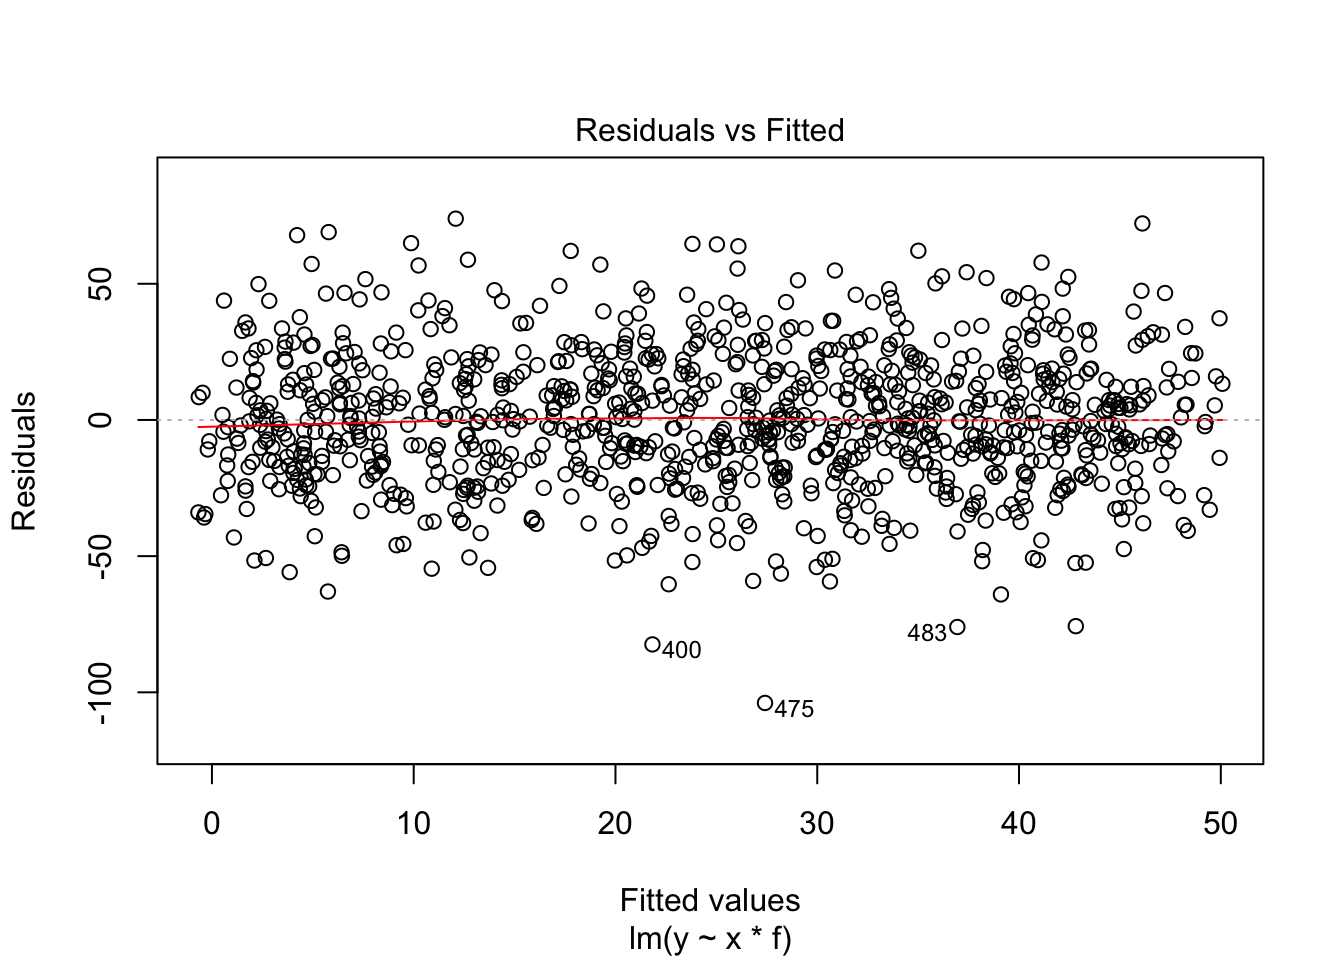
\includegraphics{RNAseq_DEGs_files/figure-latex/unnamed-chunk-52-1.pdf}

\subsection{Customised thresholds}\label{customised-thresholds}

Like in the \textbf{DESeq2} analysis, \textbf{edgeR} allows to calculate
p-values for the alternative hypothesis of at least \textbf{2 fold
difference} at \textbf{FDR 0.01}. Like in the \textbf{DESeq2} analysis,
this improves the p-values distribution and reduces the number of
suggested DEGs to less than 10\% of the genes:

\begin{Shaded}
\begin{Highlighting}[]
\CommentTok{# Calculate significance for 2-fold change}
\NormalTok{edgeR_fc2 <-}\StringTok{ }\KeywordTok{glmTreat}\NormalTok{(fit, }\DataTypeTok{coef =} \KeywordTok{ncol}\NormalTok{(design), }\DataTypeTok{lfc =} \DecValTok{1}\NormalTok{)}

\CommentTok{# Extract data for all genes}
\NormalTok{edgeR_fc2_all_genes <-}\StringTok{ }\KeywordTok{topTags}\NormalTok{(edgeR_fc2, }\DataTypeTok{n =} \KeywordTok{nrow}\NormalTok{(dgl), }\DataTypeTok{sort.by =} \StringTok{"none"}\NormalTok{)}

\CommentTok{# Check distribution of all p-values}
\KeywordTok{hist}\NormalTok{(edgeR_fc2_all_genes}\OperatorTok{$}\NormalTok{table}\OperatorTok{$}\NormalTok{PValue)}
\end{Highlighting}
\end{Shaded}

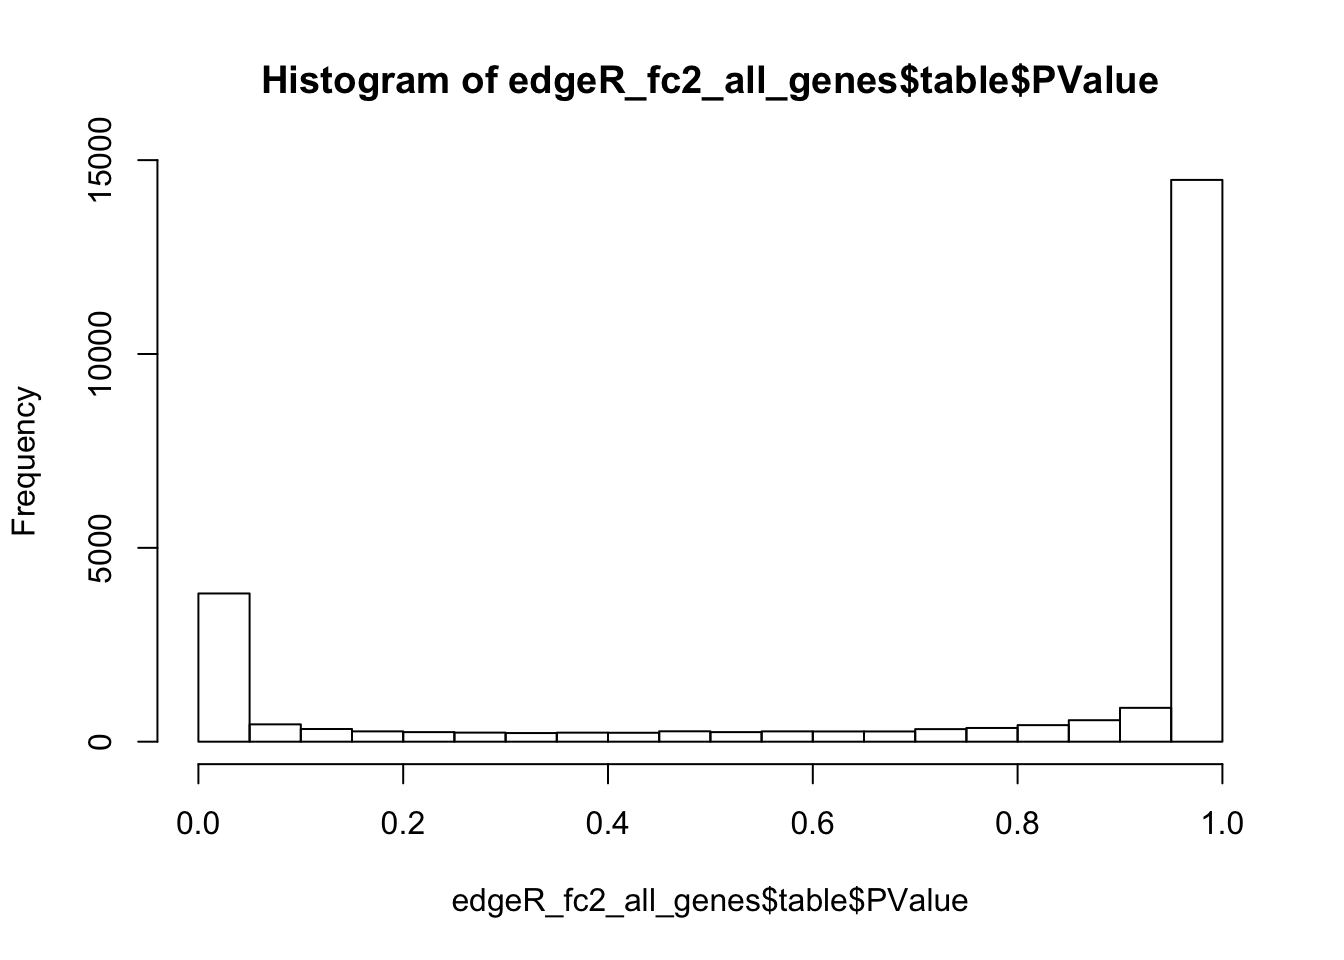
\includegraphics{RNAseq_DEGs_files/figure-latex/unnamed-chunk-53-1.pdf}

\begin{Shaded}
\begin{Highlighting}[]
\CommentTok{# Select DEGs with FDR<0.01}
\NormalTok{edgeR_fc2_fdr_}\FloatTok{0.01}\NormalTok{ <-}\StringTok{ }\KeywordTok{topTags}\NormalTok{(edgeR_fc2, }\DataTypeTok{n =} \KeywordTok{nrow}\NormalTok{(dgl), }\DataTypeTok{p.value =} \FloatTok{0.01}\NormalTok{)}

\CommentTok{# Count DEGs}
\KeywordTok{dim}\NormalTok{(edgeR_fc2_fdr_}\FloatTok{0.01}\OperatorTok{$}\NormalTok{table)}
\end{Highlighting}
\end{Shaded}

\begin{verbatim}
## [1] 2345    7
\end{verbatim}

\begin{Shaded}
\begin{Highlighting}[]
\CommentTok{# MA plot}
\KeywordTok{plotSmear}\NormalTok{(edgeR_fc2, }\DataTypeTok{de.tags =}\NormalTok{ edgeR_fc2_fdr_}\FloatTok{0.01}\OperatorTok{$}\NormalTok{table}\OperatorTok{$}\NormalTok{gene_id,}
          \DataTypeTok{main=}\StringTok{"edgeR: 2-fold change at FDR 0.01"}\NormalTok{)}
\end{Highlighting}
\end{Shaded}

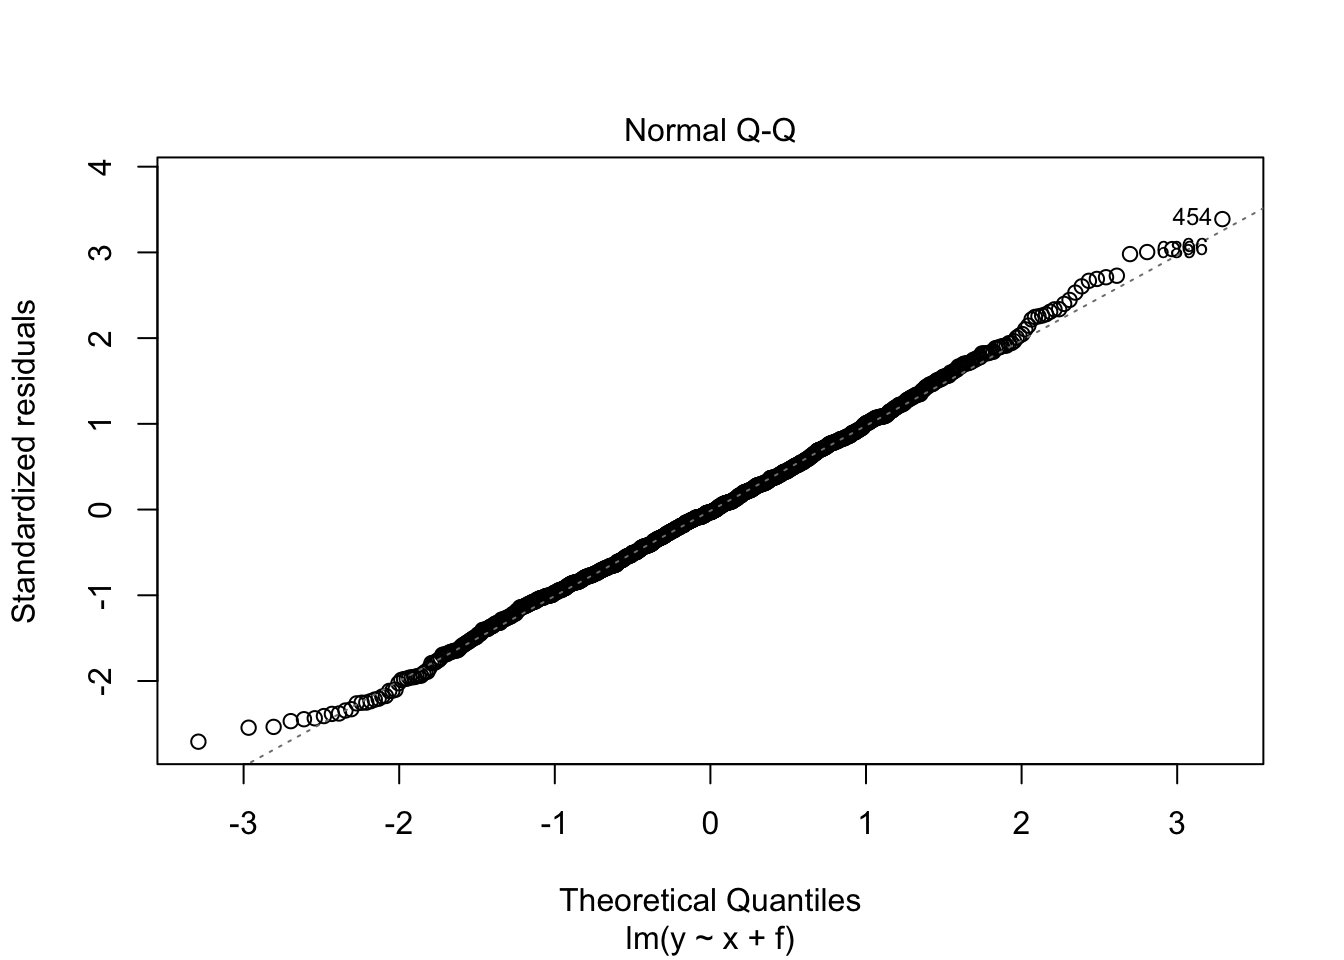
\includegraphics{RNAseq_DEGs_files/figure-latex/unnamed-chunk-53-2.pdf}

\begin{Shaded}
\begin{Highlighting}[]
\CommentTok{# Clean-up}
\KeywordTok{rm}\NormalTok{(edgeR_any_change, edgeR_any_change_all_genes, edgeR_any_change_fdr_}\FloatTok{0.1}\NormalTok{)}
\end{Highlighting}
\end{Shaded}

\subsection{Check known genes}\label{check-known-genes-1}

Like in \textbf{DESeq2} analysis, the list of DEGs suggested by
\textbf{edgeR} includes selected known genes, which expression is
associated with ER in breast cancer:

\begin{Shaded}
\begin{Highlighting}[]
\CommentTok{# List of selected previously known genes of interest}
\NormalTok{selected_known_genes=}\KeywordTok{c}\NormalTok{(}\StringTok{"ESR1"}\NormalTok{, }\StringTok{"PGR"}\NormalTok{, }\StringTok{"TFF1"}\NormalTok{, }\StringTok{"TFF3"}\NormalTok{, }\StringTok{"GATA3"}\NormalTok{, }\StringTok{"FOXA1"}\NormalTok{, }\StringTok{"FOXC1"}\NormalTok{, }\StringTok{"MIA"}\NormalTok{)}

\CommentTok{# Look at the genes of interest in the edgeR DEGs}
\NormalTok{edgeR_fc2_fdr_}\FloatTok{0.01}\OperatorTok{$}\NormalTok{table }\OperatorTok\StringTok{ }
\StringTok{  }\KeywordTok{filter}\NormalTok{(gene_name }\OperatorTok\StringTok{ }\NormalTok{selected_known_genes)}
\end{Highlighting}
\end{Shaded}

\begin{verbatim}
##              gene_id gene_name     logFC unshrunk.logFC   logCPM       PValue          FDR
## 1  ENSG00000054598.6     FOXC1 -3.702670      -3.702971 4.900554 5.479376e-43 8.342693e-40
## 2 ENSG00000091831.20      ESR1  4.428545       4.428643 8.928694 4.484183e-23 8.152178e-21
## 3  ENSG00000261857.5       MIA -3.856874      -3.858896 2.278226 1.154317e-19 1.434710e-17
## 4 ENSG00000107485.14     GATA3  2.766902       2.766926 9.178419 1.539914e-17 1.506580e-15
## 5  ENSG00000129514.5     FOXA1  2.814738       2.814787 8.249821 8.375199e-13 4.445060e-11
## 6 ENSG00000082175.13       PGR  3.617757       3.617892 7.617047 2.641659e-10 9.206504e-09
## 7  ENSG00000160182.2      TFF1  4.454900       4.455097 8.046632 2.002155e-09 6.058944e-08
## 8 ENSG00000160180.15      TFF3  3.462370       3.462466 8.112775 5.373016e-08 1.289577e-06
\end{verbatim}

\begin{Shaded}
\begin{Highlighting}[]
\CommentTok{# Clean-up}
\KeywordTok{rm}\NormalTok{(selected_known_genes)}
\end{Highlighting}
\end{Shaded}

\section{Save results}\label{save-results-1}

\textbf{write.table} function can be used to save DEGs (and results for
all genes) to text files:

\begin{Shaded}
\begin{Highlighting}[]
\CommentTok{# Save DEGs}
\KeywordTok{write.table}\NormalTok{(edgeR_fc2_fdr_}\FloatTok{0.01}\OperatorTok{$}\NormalTok{table, }
            \DataTypeTok{file=}\KeywordTok{file.path}\NormalTok{(base_folder,}\StringTok{"analysis"}\NormalTok{,}\StringTok{"results"}\NormalTok{,}\StringTok{"edgeR_fc_2_fdr_0_01_DEGs.txt"}\NormalTok{),}
            \DataTypeTok{quote=}\NormalTok{F, }\DataTypeTok{sep=}\StringTok{"}\CharTok{\textbackslash{}t}\StringTok{"}\NormalTok{, }\DataTypeTok{row.names =}\NormalTok{ F)}

\CommentTok{# Save all genes}
\KeywordTok{write.table}\NormalTok{(edgeR_fc2_all_genes}\OperatorTok{$}\NormalTok{table, }
            \DataTypeTok{file=}\KeywordTok{file.path}\NormalTok{(base_folder,}\StringTok{"analysis"}\NormalTok{,}\StringTok{"results"}\NormalTok{,}\StringTok{"edgeR_fc_2_fdr_0_01_all_genes.txt"}\NormalTok{),}
            \DataTypeTok{quote=}\NormalTok{F, }\DataTypeTok{sep=}\StringTok{"}\CharTok{\textbackslash{}t}\StringTok{"}\NormalTok{, }\DataTypeTok{row.names =}\NormalTok{ F)}
\end{Highlighting}
\end{Shaded}

\chapter{Compare DEG lists}\label{compare-deg-lists}

In this section we will compare DEGs, sugested by DESeq2 and edgeR for
at least 2 fold changes at FDR 0.01.

\section{Venn diagram}\label{venn-diagram}

\textbf{Venn diagram} allows a visual assessment of the lists overlap.

\begin{Shaded}
\begin{Highlighting}[]
\CommentTok{# Library for plotting Venn diagram}
\CommentTok{# install.packages("VennDiagram") }
\KeywordTok{suppressWarnings}\NormalTok{(}\KeywordTok{suppressMessages}\NormalTok{(}\KeywordTok{library}\NormalTok{(VennDiagram)))}

\CommentTok{# Prepare data}
\NormalTok{venn_data <-}\StringTok{ }\KeywordTok{list}\NormalTok{(}\DataTypeTok{DESEq2=}\NormalTok{DESeq2_fc_2_fdr_}\FloatTok{0.}\NormalTok{01_DEGs.df}\OperatorTok{$}\NormalTok{gene_id,}
                  \DataTypeTok{edgeR=}\NormalTok{edgeR_fc2_fdr_}\FloatTok{0.01}\OperatorTok{$}\NormalTok{table}\OperatorTok{$}\NormalTok{gene_id)}
\CommentTok{# Make plot}
\CommentTok{# (use a real file name to direct the output into a file)}
\NormalTok{venn.plot <-}\StringTok{ }\KeywordTok{venn.diagram}\NormalTok{( venn_data, }\DataTypeTok{filename =} \OtherTok{NULL}\NormalTok{,}
                           \DataTypeTok{main=}\StringTok{"DESeq2 vs edgeR"}\NormalTok{, }
                           \DataTypeTok{main.fontface=}\StringTok{"bold"}\NormalTok{,}
                           \DataTypeTok{sub=}\StringTok{"FC>2, FDR<0.01"}\NormalTok{,}
                           \DataTypeTok{col=}\KeywordTok{c}\NormalTok{(}\StringTok{"red"}\NormalTok{,}\StringTok{"blue"}\NormalTok{),}
                           \DataTypeTok{fill=}\KeywordTok{c}\NormalTok{(}\StringTok{"red"}\NormalTok{,}\StringTok{"blue"}\NormalTok{),}
                           \DataTypeTok{alpha=}\FloatTok{0.3}\NormalTok{)}
\KeywordTok{grid.newpage}\NormalTok{()}
\KeywordTok{grid.draw}\NormalTok{(venn.plot)}
\end{Highlighting}
\end{Shaded}

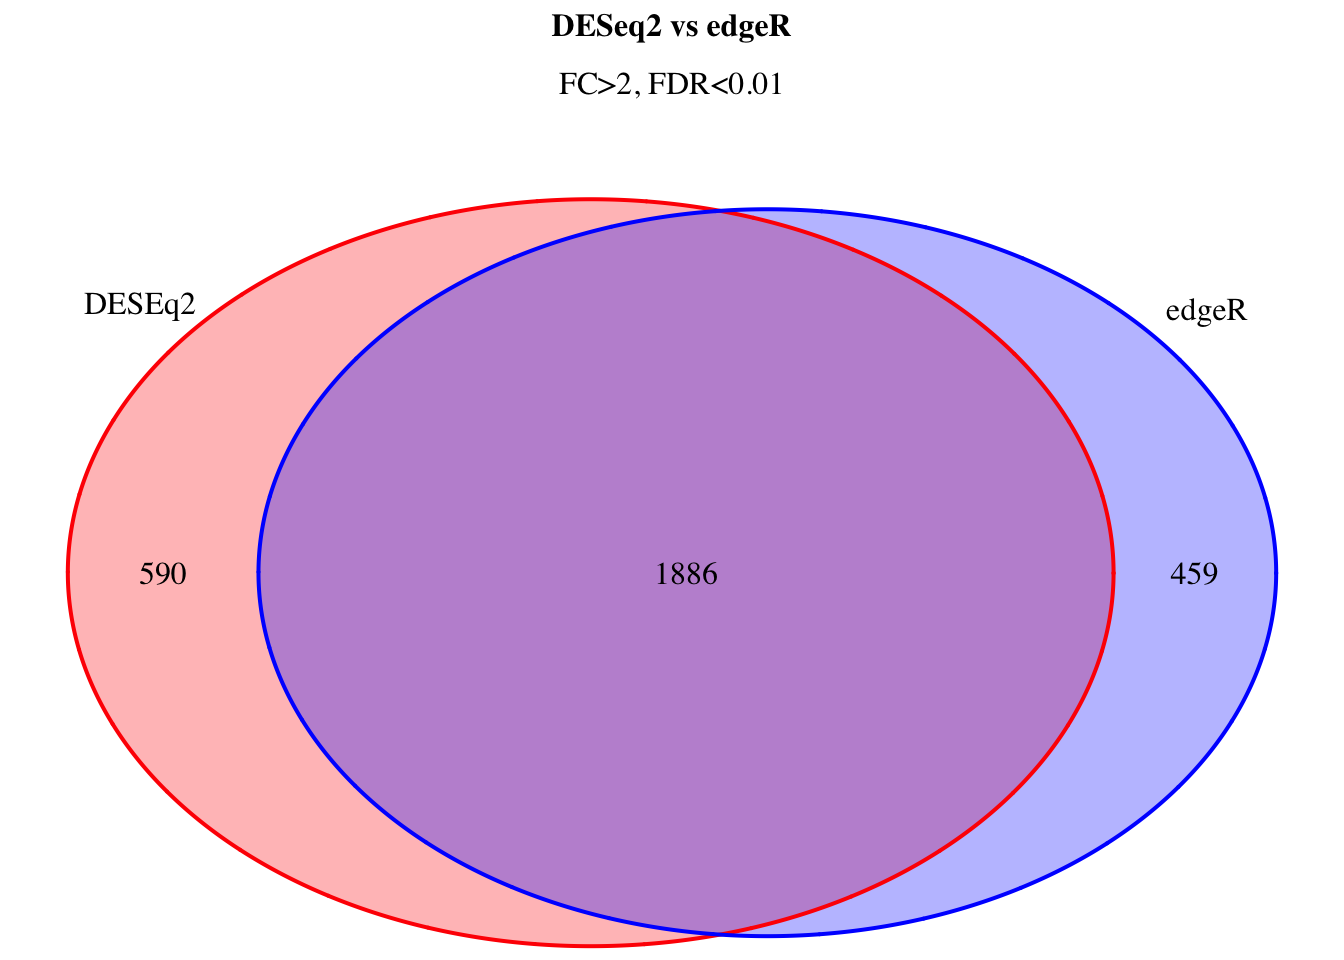
\includegraphics{RNAseq_DEGs_files/figure-latex/unnamed-chunk-58-1.pdf}

\begin{Shaded}
\begin{Highlighting}[]
\KeywordTok{grid.newpage}\NormalTok{()}

\CommentTok{# Clean-up}
\KeywordTok{rm}\NormalTok{(venn_data, venn.plot)}
\end{Highlighting}
\end{Shaded}

\section{Compare FC and FDR
estimates}\label{compare-fc-and-fdr-estimates}

The plots show a good agreement between fold-change estimates between
\textbf{DESeq2} and \textbf{edgeR} packages. The FDR estimates also show
reasonable correlation. However, it could be noted that, overall,
\textbf{edgeR} FDR estimates are more conservative for some genes in our
dataset.

\begin{Shaded}
\begin{Highlighting}[]
\CommentTok{# Estimate the size of DESEq and edgeR data for all genes}
\KeywordTok{dim}\NormalTok{(DESeq2_fc_2_fdr_}\FloatTok{0.}\NormalTok{01_all_genes.df)}
\end{Highlighting}
\end{Shaded}

\begin{verbatim}
## [1] 28362     8
\end{verbatim}

\begin{Shaded}
\begin{Highlighting}[]
\KeywordTok{dim}\NormalTok{(edgeR_fc2_all_genes}\OperatorTok{$}\NormalTok{table)}
\end{Highlighting}
\end{Shaded}

\begin{verbatim}
## [1] 24361     7
\end{verbatim}

\begin{Shaded}
\begin{Highlighting}[]
\CommentTok{# Merge DESEq and edgeR data for all genes}
\NormalTok{all_genes_intersect.df <-}\StringTok{ }\KeywordTok{inner_join}\NormalTok{(DESeq2_fc_2_fdr_}\FloatTok{0.}\NormalTok{01_all_genes.df, }
\NormalTok{                   edgeR_fc2_all_genes}\OperatorTok{$}\NormalTok{table,}
                   \DataTypeTok{by=}\StringTok{"gene_id"}\NormalTok{)}

\CommentTok{# Check result}
\KeywordTok{dim}\NormalTok{(all_genes_intersect.df)}
\end{Highlighting}
\end{Shaded}

\begin{verbatim}
## [1] 24361    14
\end{verbatim}

\begin{Shaded}
\begin{Highlighting}[]
\KeywordTok{colnames}\NormalTok{(all_genes_intersect.df)}
\end{Highlighting}
\end{Shaded}

\begin{verbatim}
##  [1] "baseMean"       "log2FoldChange" "lfcSE"          "stat"           "pvalue"         "padj"           "gene_id"        "gene_name.x"    "gene_name.y"    "logFC"          "unshrunk.logFC" "logCPM"         "PValue"         "FDR"
\end{verbatim}

\begin{Shaded}
\begin{Highlighting}[]
\CommentTok{# Select columns}
\NormalTok{all_genes_intersect.df <-}\StringTok{ }\NormalTok{all_genes_intersect.df }\OperatorTok\StringTok{ }
\StringTok{  }\KeywordTok{select}\NormalTok{(}\DataTypeTok{gene_name=}\NormalTok{gene_name.x,}
\NormalTok{         gene_id, }
         \DataTypeTok{DESeq2_lfc=}\NormalTok{log2FoldChange,}
         \DataTypeTok{DESeq2_fdr=}\NormalTok{padj,}
         \DataTypeTok{edgeR_lfc=}\NormalTok{logFC,}
         \DataTypeTok{edgeR_fdr=}\StringTok{"FDR"}\NormalTok{)}

\CommentTok{# Compare fold change}
\KeywordTok{plot}\NormalTok{(DESeq2_lfc}\OperatorTok{~}\NormalTok{edgeR_lfc, }
     \DataTypeTok{data=}\NormalTok{all_genes_intersect.df,}
     \DataTypeTok{main=}\StringTok{"LFC: DESeq2 vs edgeR"}\NormalTok{)}
\KeywordTok{abline}\NormalTok{(}\DecValTok{0}\NormalTok{,}\DecValTok{1}\NormalTok{, }\DataTypeTok{lty=}\DecValTok{2}\NormalTok{, }\DataTypeTok{col=}\StringTok{"red"}\NormalTok{)}
\end{Highlighting}
\end{Shaded}

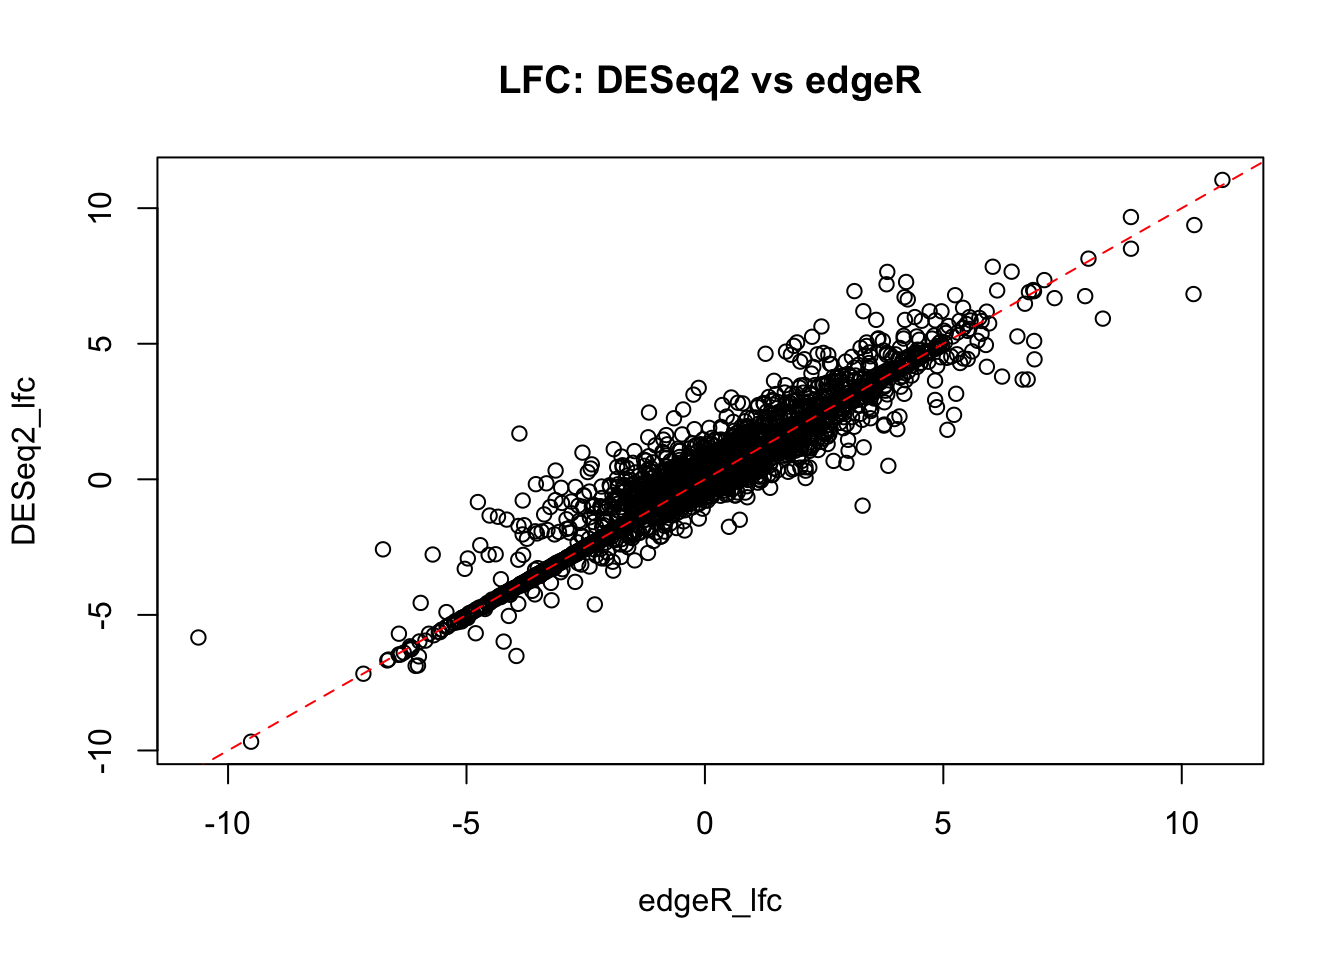
\includegraphics{RNAseq_DEGs_files/figure-latex/unnamed-chunk-59-1.pdf}

\begin{Shaded}
\begin{Highlighting}[]
\CommentTok{# Compare adjusted p (FDR)}
\KeywordTok{plot}\NormalTok{(}\KeywordTok{log}\NormalTok{(DESeq2_fdr)}\OperatorTok{~}\KeywordTok{log}\NormalTok{(edgeR_fdr), }
     \DataTypeTok{data=}\NormalTok{all_genes_intersect.df, }
     \DataTypeTok{xlim=}\KeywordTok{c}\NormalTok{(}\OperatorTok{-}\DecValTok{100}\NormalTok{,}\DecValTok{0}\NormalTok{),}\DataTypeTok{ylim=}\KeywordTok{c}\NormalTok{(}\OperatorTok{-}\DecValTok{100}\NormalTok{,}\DecValTok{0}\NormalTok{),}
     \DataTypeTok{main=}\StringTok{"FDR: DESeq2 vs edgeR"}\NormalTok{)}
\KeywordTok{abline}\NormalTok{(}\DecValTok{0}\NormalTok{,}\DecValTok{1}\NormalTok{, }\DataTypeTok{lty=}\DecValTok{2}\NormalTok{, }\DataTypeTok{col=}\StringTok{"red"}\NormalTok{)}
\end{Highlighting}
\end{Shaded}

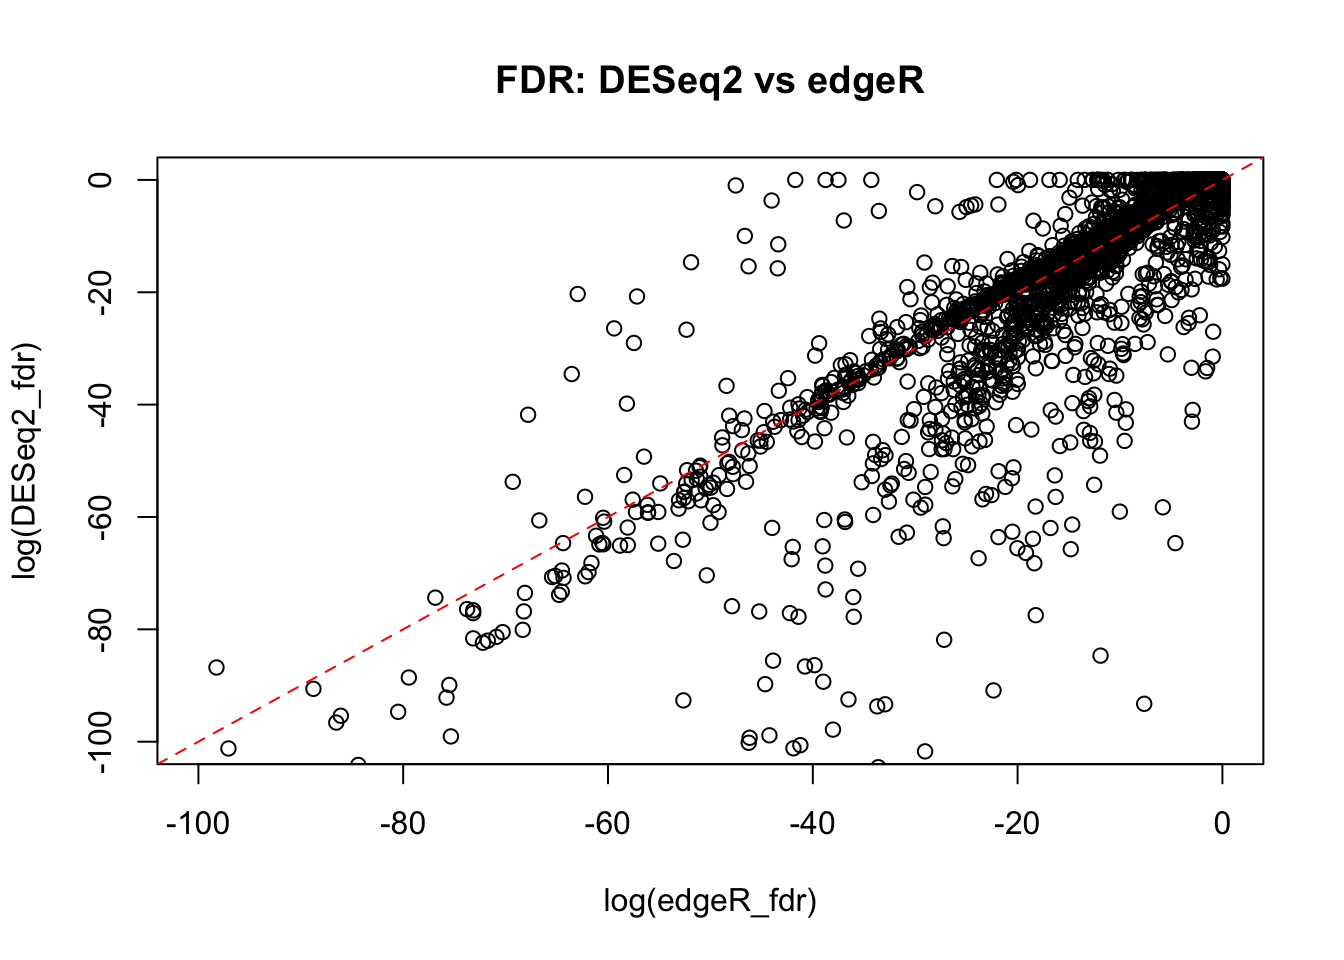
\includegraphics{RNAseq_DEGs_files/figure-latex/unnamed-chunk-59-2.pdf}

\begin{Shaded}
\begin{Highlighting}[]
\CommentTok{# Save the intersect into a text file}
\KeywordTok{write.table}\NormalTok{(all_genes_intersect.df, }
            \DataTypeTok{file=}\KeywordTok{file.path}\NormalTok{(base_folder,}\StringTok{"analysis"}\NormalTok{,}\StringTok{"results"}\NormalTok{,}\StringTok{"all_genes_intersect.txt"}\NormalTok{),}
            \DataTypeTok{quote=}\NormalTok{F, }\DataTypeTok{sep=}\StringTok{"}\CharTok{\textbackslash{}t}\StringTok{"}\NormalTok{, }\DataTypeTok{row.names =}\NormalTok{ F)}
\end{Highlighting}
\end{Shaded}

\section{DEGs intersect list}\label{degs-intersect-list}

It is reasonble to assume that the intersect between DEseq2 and edgeR
(when using the same thresholds!) shows the most robust DEGs between
ER-positive and Triple-negative breast cancer in the studied dataset.

Importantly, an external dataset is needed for an independent
confirmation of the detected DEGs.

\begin{Shaded}
\begin{Highlighting}[]
\CommentTok{# Merge DESEq and edgeR data for DEGs}
\NormalTok{DEGs_intersect.df <-}\StringTok{ }\KeywordTok{inner_join}\NormalTok{(DESeq2_fc_2_fdr_}\FloatTok{0.}\NormalTok{01_DEGs.df, }
\NormalTok{                   edgeR_fc2_fdr_}\FloatTok{0.01}\OperatorTok{$}\NormalTok{table,}
                   \DataTypeTok{by=}\StringTok{"gene_id"}\NormalTok{)}

\CommentTok{# Check result}
\KeywordTok{dim}\NormalTok{(DEGs_intersect.df)}
\end{Highlighting}
\end{Shaded}

\begin{verbatim}
## [1] 1886   11
\end{verbatim}

\begin{Shaded}
\begin{Highlighting}[]
\KeywordTok{colnames}\NormalTok{(DEGs_intersect.df)}
\end{Highlighting}
\end{Shaded}

\begin{verbatim}
##  [1] "gene_name.x"    "gene_id"        "baseMean"       "log2FoldChange" "padj"           "gene_name.y"    "logFC"          "unshrunk.logFC" "logCPM"         "PValue"         "FDR"
\end{verbatim}

\begin{Shaded}
\begin{Highlighting}[]
\CommentTok{# Select columns}
\NormalTok{DEGs_intersect.df <-}\StringTok{ }\NormalTok{DEGs_intersect.df }\OperatorTok\StringTok{ }
\StringTok{  }\KeywordTok{select}\NormalTok{(}\DataTypeTok{gene_name=}\NormalTok{gene_name.x,}
\NormalTok{         gene_id, }
         \DataTypeTok{DESeq2_lfc=}\NormalTok{log2FoldChange,}
         \DataTypeTok{DESeq2_fdr=}\NormalTok{padj,}
         \DataTypeTok{edgeR_lfc=}\NormalTok{logFC,}
         \DataTypeTok{edgeR_fdr=}\StringTok{"FDR"}\NormalTok{)}

\CommentTok{# Save the DEGs intersect into a text file}
\KeywordTok{write.table}\NormalTok{(DEGs_intersect.df, }
            \DataTypeTok{file=}\KeywordTok{file.path}\NormalTok{(base_folder,}\StringTok{"analysis"}\NormalTok{,}\StringTok{"results"}\NormalTok{,}\StringTok{"DEGs_intersect.txt"}\NormalTok{),}
            \DataTypeTok{quote=}\NormalTok{F, }\DataTypeTok{sep=}\StringTok{"}\CharTok{\textbackslash{}t}\StringTok{"}\NormalTok{, }\DataTypeTok{row.names =}\NormalTok{ F)}
\end{Highlighting}
\end{Shaded}

\chapter{Final section}\label{final-section}

Record time and objects in the environment at the end of analysis:

\begin{Shaded}
\begin{Highlighting}[]
\KeywordTok{Sys.time}\NormalTok{()}
\end{Highlighting}
\end{Shaded}

\begin{verbatim}
## [1] "2020-04-08 16:34:22 BST"
\end{verbatim}

\begin{Shaded}
\begin{Highlighting}[]
\KeywordTok{ls}\NormalTok{()}
\end{Highlighting}
\end{Shaded}

\begin{verbatim}
##  [1] "all_genes_intersect.df"            "base_folder"                       "colorize"                          "ddx"                               "DEGs_intersect.df"                 "DESeq2_fc_2_fdr_0.01_all_genes.df" "DESeq2_fc_2_fdr_0.01_DEGs.df"      "design"                            "dgl"                               "edgeR_fc2"                         "edgeR_fc2_all_genes"               "edgeR_fc2_fdr_0.01"                "fit"                               "genes.df"                          "samples.df"                        "vst_dds"
\end{verbatim}

\begin{Shaded}
\begin{Highlighting}[]
\KeywordTok{sessionInfo}\NormalTok{()}
\end{Highlighting}
\end{Shaded}

\begin{verbatim}
## R version 3.6.2 (2019-12-12)
## Platform: x86_64-apple-darwin15.6.0 (64-bit)
## Running under: macOS Catalina 10.15.4
## 
## Matrix products: default
## BLAS:   /Library/Frameworks/R.framework/Versions/3.6/Resources/lib/libRblas.0.dylib
## LAPACK: /Library/Frameworks/R.framework/Versions/3.6/Resources/lib/libRlapack.dylib
## 
## locale:
## [1] en_GB.UTF-8/en_GB.UTF-8/en_GB.UTF-8/C/en_GB.UTF-8/en_GB.UTF-8
## 
## attached base packages:
##  [1] grid      parallel  stats4    stats     graphics  grDevices utils     datasets  methods   base     
## 
## other attached packages:
##  [1] VennDiagram_1.6.20          futile.logger_1.4.3         edgeR_3.28.1                limma_3.42.2                DESeq2_1.26.0               SummarizedExperiment_1.16.1 DelayedArray_0.12.2         BiocParallel_1.20.1         matrixStats_0.56.0          Biobase_2.46.0              rtracklayer_1.46.0          GenomicRanges_1.38.0        GenomeInfoDb_1.22.1         IRanges_2.20.2              S4Vectors_0.24.3            BiocGenerics_0.32.0         dplyr_0.8.5                 knitr_1.28                 
## 
## loaded via a namespace (and not attached):
##  [1] bitops_1.0-6             bit64_0.9-7              RColorBrewer_1.1-2       tools_3.6.2              backports_1.1.6          R6_2.4.1                 rpart_4.1-15             Hmisc_4.4-0              DBI_1.1.0                colorspace_1.4-1         nnet_7.3-13              tidyselect_1.0.0         gridExtra_2.3            bit_1.1-15.2             compiler_3.6.2           cli_2.0.2                formatR_1.7              htmlTable_1.13.3         labeling_0.3             bookdown_0.18            scales_1.1.0             checkmate_2.0.0          genefilter_1.68.0        stringr_1.4.0            digest_0.6.25            Rsamtools_2.2.3          foreign_0.8-76           rmarkdown_2.1            XVector_0.26.0           base64enc_0.1-3          jpeg_0.1-8.1             pkgconfig_2.0.3          htmltools_0.4.0          htmlwidgets_1.5.1        rlang_0.4.5              rstudioapi_0.11          RSQLite_2.2.0            farver_2.0.3             acepack_1.4.1           
## [40] RCurl_1.98-1.1           magrittr_1.5             GenomeInfoDbData_1.2.2   Formula_1.2-3            Matrix_1.2-18            Rcpp_1.0.4               munsell_0.5.0            fansi_0.4.1              lifecycle_0.2.0          stringi_1.4.6            yaml_2.2.1               zlibbioc_1.32.0          blob_1.2.1               crayon_1.3.4             lattice_0.20-41          Biostrings_2.54.0        splines_3.6.2            annotate_1.64.0          locfit_1.5-9.4           pillar_1.4.3             geneplotter_1.64.0       futile.options_1.0.1     XML_3.99-0.3             glue_1.4.0               evaluate_0.14            latticeExtra_0.6-29      lambda.r_1.2.4           data.table_1.12.8        png_0.1-7                vctrs_0.2.4              gtable_0.3.0             purrr_0.3.3              assertthat_0.2.1         ggplot2_3.3.0            xfun_0.12                xtable_1.8-4             survival_3.1-11          tibble_3.0.0             GenomicAlignments_1.22.1
## [79] AnnotationDbi_1.48.0     memoise_1.1.0            cluster_2.1.0            ellipsis_0.3.0
\end{verbatim}

\end{document}
